% Arquivo LaTeX de exemplo de dissertação/tese a ser apresentada à CPG do IME-USP
%
% Criação: Jesús P. Mena-Chalco
% Revisão: Fabio Kon e Paulo Feofiloff
% Adaptação para UTF8, biblatex e outras melhorias: Nelson Lago
%
% Except where otherwise indicated, these files are distributed under
% the MIT Licence. The example text, which includes the tutorial and
% examples as well as the explanatory comments in the source, are
% available under the Creative Commons Attribution International
% Licence, v4.0 (CC-BY 4.0) - https://creativecommons.org/licenses/by/4.0/


%%%%%%%%%%%%%%%%%%%%%%%%%%%%%%%%%%%%%%%%%%%%%%%%%%%%%%%%%%%%%%%%%%%%%%%%%%%%%%%%
%%%%%%%%%%%%%%%%%%%%%%%%%%%%%%% PREÂMBULO LaTeX %%%%%%%%%%%%%%%%%%%%%%%%%%%%%%%%
%%%%%%%%%%%%%%%%%%%%%%%%%%%%%%%%%%%%%%%%%%%%%%%%%%%%%%%%%%%%%%%%%%%%%%%%%%%%%%%%

% A opção twoside (frente-e-verso) significa que a aparência das páginas pares
% e ímpares pode ser diferente. Por exemplo, as margens podem ser diferentes ou
% os números de página podem aparecer à direita ou à esquerda alternadamente.
% Mas nada impede que você crie um documento "só frente" e, ao imprimir, faça
% a impressão frente-e-verso.
%
% Aqui também definimos a língua padrão do documento
% (a última da lista) e línguas adicionais.
\documentclass[12pt,twoside,brazilian,english]{book}
%\documentclass[12pt,twoside,english,brazilian]{book}

% Ao invés de definir o tamanho das margens, vamos definir os tamanhos do
% texto, do cabeçalho e do rodapé, e deixamos a package geometry calcular
% o tamanho das margens em função do tamanho do papel. Assim, obtemos o
% mesmo resultado impresso, mas com margens diferentes, se o tamanho do
% papel for diferente.
\usepackage[a4paper]{geometry}

\geometry{
  textwidth=152mm,
  hmarginratio=12:17, % 24:34 -> com papel A4, 24mm + 152mm + 34mm = 210mm
  textheight=237mm,
  vmarginratio=8:7, % 32:28 -> com papel A4, 32mm + 237mm + 28mm = 297mm
  headsep=11mm, % distância entre a base do cabeçalho e o texto
  headheight=21mm, % qualquer medida grande o suficiente, p.ex., top - headsep
  footskip=10mm,
  marginpar=20mm,
  marginparsep=5mm,
}

% Vários pacotes e opções de configuração genéricos; para personalizar o
% resultado, modifique estes arquivos.
%%%%%%%%%%%%%%%%%%%%%%%%%%%%%%%%%%%%%%%%%%%%%%%%%%%%%%%%%%%%%%%%%%%%%%%%%%%%%%%%
%%%%%%%%%%%%%%%%%%%%%%% CONFIGURAÇÕES E PACOTES BÁSICOS %%%%%%%%%%%%%%%%%%%%%%%%
%%%%%%%%%%%%%%%%%%%%%%%%%%%%%%%%%%%%%%%%%%%%%%%%%%%%%%%%%%%%%%%%%%%%%%%%%%%%%%%%

% Vários comandos auxiliares para o desenvolvimento de packages e classes;
% aqui, usamos em alguns comandos de formatação e condicionais.
\usepackage{etoolbox}
%\RequirePackage{pdftexcmds}
\usepackage{letltxmacro}
%\usepackage{ltxcmds}

% LaTeX 3
\usepackage{expl3}
\usepackage{xparse}

% Detecta se estamos usando pdftex, luatex, xetex etc.
\usepackage{iftex}

%\usepackage{xfp} % Floating-point calculations

\usepackage{regexpatch}

% O projeto LaTeX3 renomeou algumas macros em 2019-03-05 e removeu
% a compatibilidade com os nomes antigos em 2020-07-17 a partir de
% 2021-01-01 (veja o arquivo l3deprecation.dtx e o changelog em
% https://github.com/latex3/latex3/blob/main/l3kernel/CHANGELOG.md).
% Isso afetou a package regexpatch: versões antigas da package não
% funcionam com versões novas de LaTeX e vice-versa. Infelizmente,
% ubuntu 21.04 (hirsute) e debian 11 (bullseye) incluem essas versões
% incompatíveis e, portanto, a package regexpatch não funciona nesses
% ambientes. Talvez fosse possível contornar esse problema com a
% package latexrelease, mas isso afetaria muitos outros recursos.
% Ao invés disso, vamos restaurar manualmente a compatibilidade.
% TODO: remover isto após debian bullseye se tornar obsoleta,
%       provavelmente no final de 2024.
\makeatletter
\ExplSyntaxOn

\@ifpackagelater{regexpatch}{2021/03/21}
  {} % Se regexpatch é "nova", expl3 deve ser também; nada a fazer
  {
    % Talvez o correto seja 2021/01/01, mas na prática o resultado é o mesmo
    \@ifpackagelater{expl3}{2020/07/17}
      {
        % As versões são incompatíveis; vamos recuperar as macros preteridas
        \cs_gset:Npn \token_get_prefix_spec:N { \cs_prefix_spec:N }
        \cs_gset:Npn \token_get_arg_spec:N { \cs_argument_spec:N }
        \cs_gset:Npn \token_get_replacement_spec:N { \cs_replacement_spec:N }
      }
      {} % As duas packages são antigas e, portanto, compatíveis entre si
  }
\ExplSyntaxOff
\makeatother

% Algumas packages dependem de xpatch e tentam carregá-la, causando conflitos
% com regexpatch. Como regexpatch oferece todos os recursos de xpatch (ela
% é uma versão estendida de xpatch, mas ainda considerada experimental), vamos
% fazê-las acreditar que xpatch já foi carregada.
\expandafter\xdef\csname ver@xpatch.sty\endcsname{2012/10/02}

% Acrescenta a correção deste bug (contida na release 2018-11-28):
% https://github.com/latex3/latex2e/issues/94 . Se a correção não
% puder ser aplicada, temos uma versão de LaTeX que já a incorpora.
% Esse bug afeta apenas textos em duas colunas.
% TODO: remover após ubuntu 18.04 se tornar obsoleta (abril/2023)
\makeatletter
\patchcmd\@combinedblfloats{\box\@outputbox}{\unvbox\@outputbox}{}{}
\makeatother

% Arithmetic expressions in \set{length,counter} & \addto{length,counter};
% commands \widthof, \heightof, \depthof, \totalheightof, \settototalheight
\usepackage{calc}

% Algumas packages "padrão" da AMS, que são praticamente obrigatórias.
% Algumas delas devem ser carregadas antes de unicode-math ou das
% definições das fontes do documento. É preciso carregar amsthm após
% amsmath para o comando \qedhere funcionar dentro do ambiente align.
\usepackage{amssymb}
\usepackage{amsmath}
\usepackage{amsthm}

% "fontenc" é um parâmetro do NFSS (sistema de gestão de fontes do
% LaTeX; consulte "texdoc fntguide" e "texdoc fontenc"). O default
% é OT1, mas ele tem algumas limitações; a mais importante é que,
% com ele, palavras acentuadas não podem ser hifenizadas. Por
% conta disso, quase todos os documentos LaTeX utilizam o fontenc
% T1. A escolha do fontenc tem consequências para as fontes que
% podem ser usadas com NFSS; hoje em dia T1 tem mais opções de
% qualidade, então não se perde nada em usá-lo. A package fontspec
% (para gestão de fontes usando outro mecanismo, compatível apenas
% com lualatex e xelatex) carrega fontenc automaticamente, mas
% usando outra codificação ("TU" e não "T1"). Ainda assim, é útil
% carregar o fontenc T1 (antes de carregar fontspec!) para o caso
% de alguma fonte "antiga" ser utilizada no documento (embora isso
% não seja recomendado: lualatex e xelatex só são capazes de
% hifenizar palavras acentuadas com o fontenc TU).
\usepackage[T1]{fontenc}

\ifPDFTeX
  % O texto está escrito em utf8.
  \usepackage[utf8]{inputenc}

  % Permitem utilizar small caps + itálico (e outras pequenas
  % melhorias). Em geral, desnecessário com fontspec, a menos
  % que alguma package utilize especificamente. Algumas raras
  % packages de fontes podem causar conflitos com fontaxes, em
  % geral por utilizarem a package "concorrente" nfssext-cfr.
  \usepackage{fontaxes}
  \usepackage{mweights}

  % LaTeX substitui algumas sequências de caracteres, como
  % "fi", "fl" e outras, por caracteres especiais ("ligaduras").
  % Para que seja possível fazer copiar/colar ou buscas por
  % textos contendo essas ligaduras, o arquivo PDF precisa
  % conter uma tabela indicando quais são elas. Com fontes
  % OTF (LuaLaTeX ou XeLaTeX) isso não costuma ser um problema,
  % mas com pdfLaTeX pode ser. Estes dois comandos (que só
  % existem no pdfLaTeX) incluem uma tabela genérica que
  % funciona para a maioria das fontes. Veja a seção 5 de
  % http://www.tug.org/TUGboat/Articles/tb29-1/tb91thanh-fonts.pdf
  % Note que alguns visualizadores de PDF tentam "adivinhar"
  % o conteúdo da tabela quando ela está incompleta ou não
  % existe, então copiar/colar e buscas podem funcionar em
  % alguns visualizadores e em outros não.
  \input glyphtounicode.tex
  \pdfgentounicode=1
\else
  % Não é preciso carregar inputenc com LuaTeX e XeTeX, pois
  % com eles utf8 é obrigatório.
  \usepackage{fontspec}

  % Ao invés de usar o sistema tradicional de LaTeX para gerir
  % as fontes matemáticas, utiliza as extensões matemáticas do
  % formato otf definidas pela microsoft. Ao ativar esta package
  % o mecanismo tradicional não funciona mais! Há poucas fontes
  % com suporte a unicode-math.
  \usepackage{unicode-math}
\fi

% Acesso a símbolos adicionais, como \textrightarrow, \texteuro etc.,
% disponíveis na maioria das fontes através do fontenc TS1 ou mudando
% momentaneamente para computer modern/latin modern. Raramente útil
% com lualatex/xelatex, mas não causa problemas. Várias packages de
% fontes carregam textcomp, às vezes com opções específicas; assim,
% para evitar problemas, vamos carregá-la no final do preâmbulo para
% o caso de ela não ter sido carregada antes.
\AtBeginDocument{\usepackage{textcomp}}

% TeXLive 2018 inclui a versão 2.7a da package microtype e a versão
% 1.07 de luatex. Essa combinação faz aparecer um bug:
% https://tex.stackexchange.com/questions/476740/microtype-error-with-lualatex-attempt-to-call-field-warning-a-nil-value
% Aqui, aplicamos a solução sugerida, que não tem "contra-indicações".
\ifLuaTeX
  \usepackage{luatexbase}
\fi

% microajustes no tamanho das letras, espaçamento etc. para melhorar
% a qualidade visual do resultado.
\usepackage{microtype}

% Alguns "truques" (sujos?) para minimizar over/underfull boxes.
%
% Para fazer um texto justificado, é preciso modificar o tamanho dos espaços
% em cada linha para mais ou para menos em relação ao seu tamanho ideal. Para
% escolher as quebras de linha, TeX vai percorrendo o texto procurando lugares
% possíveis para quebrar as linhas considerando essa flexibilidade mas dentro
% de um certo limite mínimo/máximo. Nesse processo, ele associa a cada possível
% linha o valor *badness*, que é o nível de distorção do tamanho dos espaços
% daquela linha em relação ao ideal, e ignora opções que tenham badness muito
% grande (esse limite é dado por \tolerance). Depois de encontradas todas
% as possíveis quebras de linha e a badness de cada uma, TeX calcula as
% *penalties* das quebras encontradas, que são uma medida de quebras "ruins".
% Por exemplo, na configuração padrão, quebrar uma linha hifenizando uma
% palavra gera uma penalty de 50; já uma quebra que faça a última linha
% do parágrafo ficar sozinha na página seguinte gera uma penalty de 150.
% Finalmente, TeX calcula a "feiúra" de cada possível linha (demerits)
% com base na badness e nas penalties e escolhe a solução que minimiza os
% demerits totais do parágrafo. Os comandos \linebreak e \pagebreak funcionam
% simplesmente acrescentando uma penalty negativa ao lugar desejado para a
% quebra.
%
% Para cada fonte, o espaço entre palavras tem um tamanho ideal, um
% tamanho mínimo e um tamanho máximo (é possível obter os valores com
% \number\fontdimenX\font\relax, veja
% https://tex.stackexchange.com/questions/88991/what-do-different-fontdimennum-mean ).
% TeX nunca reduz um espaço para menos que o mínimo da fonte, mas pode
% aumentá-lo para mais que o máximo. Se os espaços de uma linha ficam
% com o tamanho ideal, a badness da linha é 0; se o tamanho é
% reduzido/aumentado 50% do mínimo/máximo, a badness da linha é 12; se
% o tamanho é reduzido/aumentado para o mínimo/máximo, a badness é 100,
% e assim por diante. O valor máximo possível para badness é 10.000, que
% significa "badness infinita". Como é feito o cálculo: se as medidas
% do espaço definidas pela fonte são "x plus y minus z" e o tamanho
% final do espaço é "x + k*y" ou "x - k*z", a badness é 100*(k^3). Com
% Libertinus corpo 12, os valores são "3pt plus 1.5pt minus .9996pt",
% Então se o espaço tiver sido aumentado para 3.75pt, o fator é 0.5 e
% a badness é 100*(.5^3) = 12.
%
% \tolerance indica a badness máxima que TeX aceita para uma linha; seu valor
% default é 200. Assim, aumentar para, digamos, 300 ou 400, permite que
% TeX escolha parágrafos com maior variação no espaçamento entre as palavras.
% No entanto, no cálculo de demerits, a badness e as penalties de cada linha
% são elevadas ao quadrado, então TeX geralmente prefere escolher outras
% opções no lugar de uma linha com espaçamento ruim. Por exemplo, órfãs/viúvas
% têm demerit de 22.500 e dois hífens seguidos têm demerit de 10.000; já uma
% linha com badness 400 tem demerit 160.000. Portanto, não é surpreendente que
% a maioria dos parágrafos tenha demerits abaixo de 40.000, quase todos abaixo
% de 100.000 e praticamente nenhum acima de 1.000.000. Isso significa que, para
% a grande maioria dos parágrafos, aumentar \tolerance não faz diferença: uma
% linha com badness 400 nunca será efetivamente escolhida se houver qualquer
% outra opção com badness menor. Também fica claro que não há muita diferença
% real entre definir \tolerance como 800 ou 9.999 (a não ser fazer TeX
% trabalhar mais desnecessariamente).
%
% O problema muda de figura se TeX não consegue encontrar uma solução. Isso
% pode acontecer em dois casos: (1) o parágrafo tem ao menos uma linha que não
% pode ser quebrada com badness < 10.000 ou (2) o parágrafo tem ao menos uma
% linha que não pode ser quebrada com badness < tolerance (mas essa badness é
% menor que 10.000).
%
% No primeiro caso, se houver várias possibilidades de linhas que não podem ser
% quebradas, TeX não vai ser capaz de compará-las e escolher a melhor: todas
% têm a badness máxima (10.000) e, portanto, a que gerar menos deméritos no
% restante do parágrafo será a escolhida. Na realidade, no entanto, essas
% linhas *não* são igualmente ruins entre si, o que pode levar TeX a fazer uma
% má escolha. Para evitar isso, TeX tenta novamente aplicando
% \emergencystretch, que "faz de conta" que o tamanho máximo ideal dos espaços
% da linha é maior que o definido na fonte. Isso reduz a badness de todas as
% linhas, o que soa parecido com aumentar \tolerance. Há três diferenças, no
% entanto: (1) essa mudança só afeta os parágrafos que falharam; (2) soluções
% que originalmente teriam badness = 10.000 (e, portanto, seriam vistas como
% equivalentes) podem ser avaliadas e comparadas entre si; e (3) como a badness
% de todas as linhas diminui, a possibilidade de outras linhas que
% originalmente tinham badness alta serem escolhidas aumenta. Esse último ponto
% significa que \emergencystretch pode fazer TeX escolher linhas mais
% espaçadas, fazendo o espaçamento do parágrafo inteiro aumentar e, portanto,
% tornando o resultado mais homogêneo mesmo com uma linha particularmente ruim.
%
% É esse último ponto que justifica o uso de \emergencystretch no segundo caso
% também: apenas aumentar a tolerância, nesse caso, poderia levar TeX a
% diagramar uma linha ruim em meio a um parágrafo bom, enquanto
% \emergencystretch pode fazer TeX aumentar o espaçamento de maneira geral no
% parágrafo, minimizando o contraste da linha problemática com as demais.
% Colocando a questão de outra maneira, aumentar \tolerance para lidar com
% esses parágrafos problemáticos pode fazê-los ter uma linha especialmente
% ruim, enquanto \emergencystretch pode dividir o erro entre várias linhas.
% Assim, definir \tolerance em torno de 800 parece razoável: no caso geral,
% não há diferença e, se um desses casos difíceis não pode ser resolvido com
% uma linha de badness até 800, \emergencystretch deve ser capaz de gerar um
% resultado igual ou melhor.
%
% Penalties & demerits: https://tex.stackexchange.com/a/51264
% Definições (fussy, sloppy etc.): https://tex.stackexchange.com/a/241355
% Mais definições (hfuzz, hbadness etc.): https://tex.stackexchange.com/a/50850
% Donald Arseneau defendendo o uso de \sloppy: https://groups.google.com/d/msg/comp.text.tex/Dhf0xxuQ66E/QTZ7aLYrdQUJ
% Artigo detalhado sobre \emergencystretch: https://www.tug.org/TUGboat/tb38-1/tb118wermuth.pdf
% Esse artigo me leva a crer que algo em torno de 1.5em é suficiente

\tolerance=800
\hyphenpenalty=100 % Default 50; se o texto é em 2 colunas, 50 é melhor
\setlength{\emergencystretch}{1.5em}

% Não gera warnings para Overfull menor que 1pt
\hfuzz=1pt
\vfuzz\hfuzz

% Não gera warnings para Underfull com badness < 1000
\hbadness=1000
\vbadness=1000

% Por padrão, o algoritmo LaTeX para textos não-justificados é (muito) ruim;
% este pacote implementa um algoritmo bem melhor
\usepackage[newcommands]{ragged2e}

% ragged2e funciona porque permite que LaTeX hifenize palavras em textos
% não-justificados quando necessário. No caso de textos centralizados,
% no entanto, isso em geral não é desejável. Assim, newcommands não é
% interessante para \centering e \begin{center}. newcommands também
% causa problemas com legendas se o float correspondente usa \centering
% (o que é muito comum). Assim, vamos voltar \centering e \begin{center}
% à definição padrão.
\let\centering\LaTeXcentering
\let\center\LaTeXcenter
\let\endcenter\endLaTeXcenter

% Com ragged2e e a opção "newcommands", textos curtos não-justificados
% podem gerar warnings sobre "underfull \hbox". Não há razão para pensar
% muito nesses warnings, então melhor desabilitá-los.
% https://tex.stackexchange.com/questions/17659/ragged2e-newcommands-option-produces-underfull-hbox-warnings
\makeatletter
\gappto{\raggedright}{\hbadness=\@M}
\gappto{\RaggedRight}{\hbadness=\@M}
\gappto{\raggedleft}{\hbadness=\@M}
\gappto{\RaggedLeft}{\hbadness=\@M}
\gappto{\Centering}{\hbadness=\@M} % not \centering
\gappto{\flushleft}{\hbadness=\@M}
\gappto{\FlushLeft}{\hbadness=\@M}
\gappto{\flushright}{\hbadness=\@M}
\gappto{\FlushRight}{\hbadness=\@M}
\gappto{\Center}{\hbadness=\@M} % not \center
\makeatother

% Espaçamento entre linhas configurável (\singlespacing, \onehalfspacing etc.)
\usepackage{setspace}

% LaTeX às vezes coloca notas de rodapé logo após o final do texto da
% página ao invés de no final da página; este pacote evita isso e faz
% notas de rodapé funcionarem corretamente em títulos de seções.
% Esta package deve ser carregada depois de setspace.
\usepackage[stable,bottom]{footmisc}

% Se uma página está vazia, não imprime número de página ou cabeçalho
\usepackage{emptypage}

% hyperref deve preferencialmente ser carregada próximo ao final
% do preâmbulo mas, para o caso de alguma package forçar a sua
% carga antes de executarmos \usepackage explicitamente, vamos
% garantir que estas opções estejam ativas.
\PassOptionsToPackage{
  unicode=true,
  pdfencoding=unicode,
  plainpages=false,
  pdfpagelabels,
  bookmarksopen=true,
  breaklinks=true,
  %hyperfootnotes=false, % polui desnecessariamente com bordercolor
}{hyperref}

% Carrega nomes de cores disponíveis (podem ser usados com hyperref e listings)
\usepackage[hyperref,svgnames,x11names,table]{xcolor}

% LaTeX define os comandos "MakeUppercase" e "MakeLowercase", mas eles têm
% algumas limitações; esta package define os comandos MakeTextUppercase e
% MakeTextLowercase que resolvem isso.
\usepackage{textcase}

% Em documentos frente-e-verso, LaTeX faz o final da página terminar sempre
% no mesmo lugar (exceto no final dos capítulos). Esse comportamento pode ser
% ativado explicitamente com o comando "\flushbottom". Mas se, por alguma
% razão, o volume de texto na página é "pequeno", essa página vai ter espaços
% verticais artificialmente grandes. Uma solução para esse problema é utilizar
% "\raggedbottom" (padrão em documentos que não são frente-e-verso): com essa
% opção, as páginas podem terminar em alturas ligeiramente diferentes. Outra
% opção é corrigir manualmente cada página problemática, por exemplo com o
% comando "\enlargethispage".
%\raggedbottom
\flushbottom

% Por padrão, LaTeX coloca uma espaço aumentado após sinais de pontuação;
% Isso não é tão bom quanto alguns TeX-eiros defendem :) .
% Esta opção desabilita isso e, consequentemente, evita problemas com
% "id est" (i.e.) e "exempli gratia" (e.g.)
\frenchspacing

% Trechos de texto "puro" (tabs, quebras de linha etc. não são modificados)
\usepackage{verbatim}

% Durante o processamento, LaTeX procura por arquivos adicionais necessários
% (tanto componentes do próprio LaTeX, como packages e fontes, quanto partes
% do conteúdo em si, como imagens carregadas com \includegraphics ou arquivos
% solicitados com \input ou \include) no diretório de instalação e também
% no diretório atual (ou seja, o diretório do projeto). Assim, normalmente
% é preciso usar caminhos relativos para incluir arquivos de subdiretórios:
% "\input{diretorio/arquivo}". No entanto, há duas limitações:
%
% 1. É necessário dizer "\input{diretorio/arquivo}" mesmo quando o arquivo
%    que contém esse comando já está dentro do subdiretório.
%
% 2. Isso não deve ser usado para packages ("\usepackage{diretorio/package}"),
%    embora na prática funcione.
%
% Há três maneiras recomendadas de resolver esses problemas:
%
% 1. Acrescentando os diretórios desejados ao arquivo texmf.cnf
%
% 2. Acrescentando os diretórios desejados às variáveis de ambiente
%    TEXINPUTS e BSTINPUTS
%
% 3. Colocando os arquivos adicionais na árvore TEXMF (geralmente, no
%    diretório texmf dentro do diretório do usuário).
%
% Essas soluções, no entanto, não podem ser automatizadas por este modelo
% e são um tanto complicadas para usuários menos experientes. Veja mais a
% respeito na seção 5 de "texdoc kpathsea" e em
% https://www.overleaf.com/learn/latex/Articles/An_introduction_to_Kpathsea_and_how_TeX_engines_search_for_files .
%
% A package import pode solucionar o primeiro problema, mas exige o uso
% de outro comando no lugar de \input, então não a usamos aqui.
%\usepackage{import}
%
% Uma solução mais simples é acrescentar os diretórios desejados à macro
% \input@path, originalmente criada para resolver um problema relacionado
% à portabilidade. Seu uso não é normalmente recomendado por razões de
% desempenho, mas no nosso caso (em que adicionamos apenas um diretório
% com poucos arquivos e com máquinas modernas) isso não é um problema. Veja
% https://tex.stackexchange.com/questions/241828/define-path-for-packages-in-the-latex-file-analog-of-inputpath-or-graphicspa#comment705011_241832
\csappto{input@path}{{extras/}}

%%%%%%%%%%%%%%%%%%%%%%%%%%%%%%%%%%%%%%%%%%%%%%%%%%%%%%%%%%%%%%%%%%%%%%%%%%%%%%%%
%%%%%%%%%%%%%%%%%%%%%%%%%%%%%%%%%%% LÍNGUAS %%%%%%%%%%%%%%%%%%%%%%%%%%%%%%%%%%%%
%%%%%%%%%%%%%%%%%%%%%%%%%%%%%%%%%%%%%%%%%%%%%%%%%%%%%%%%%%%%%%%%%%%%%%%%%%%%%%%%

\makeatletter
\ExplSyntaxOn

% We need to have at least some variant of Portuguese and of English
% loaded to generate the abstract/resumo, palavras-chave/keywords etc.
% We will make sure that both languages are present in the class options
% list by adding them if needed. With this, these options become global
% and therefore are seen by all packages (among them, babel).
%
% babel traditionally uses "portuguese", "brazilian", "portuges", or
% "brazil" to support the Portuguese language, using .ldf files. babel
% is also in the process of implementing a new scheme, using .ini
% files, based on the concept of "locales" instead of "languages". This
% mechanism uses the names "portuguese-portugal", "portuguese-brazil",
% "portuguese-pt", "portuguese-br", "portuguese", "brazilian", "pt",
% "pt-PT", and "pt-BR" (i.e., neither "portuges" nor "brazil"). To avoid
% compatibility problems, let's stick with "brazilian" or "portuguese"
% by substituting portuges and brazil if necessary.

\NewDocumentCommand\@IMEportugueseAndEnglish{m}{

  % Make sure any instances of "portuges" and "brazil" are replaced
  % by "portuguese" e "brazilian"; other options are unchanged.
  \seq_gclear_new:N \l_tmpa_seq
  \seq_gclear_new:N \l_tmpb_seq
  \seq_gset_from_clist:Nc \l_tmpa_seq {#1}

  \seq_map_inline:Nn \l_tmpa_seq{
    \def\@tempa{##1}
    \ifstrequal{portuges}{##1}
      {
        \GenericInfo{sbc2019}{}{Substituting~language~portuges~->~portuguese}
        \def\@tempa{portuguese}
      }
      {}
    \ifstrequal{brazil}{##1}
      {
        \GenericInfo{}{Substituting~language~brazil~->~brazilian}
        \def\@tempa{brazilian}
      }
      {}
    \seq_gput_right:NV \l_tmpb_seq {\@tempa}
  }

  % Remove the leftmost duplicates (default is to remove the rightmost ones).
  % Necessary in case the user did "portuges,portuguese", "brazil,brazilian"
  % or some variation: When we substitute the language, we end up with the
  % exact same language twice, which may mess up the main language selection.
  \seq_greverse:N \l_tmpb_seq
  \seq_gremove_duplicates:N \l_tmpb_seq
  \seq_greverse:N \l_tmpb_seq

  % If the user failed to select some variation of English and Portuguese,
  % we add them here. We also remember which ones of portuguese/brazilian,
  % english/american/british etc. were selected.
  \exp_args:Nnx \regex_extract_all:nnNTF
    {\b(portuguese|brazilian)\b}
    {\seq_use:Nn \l_tmpb_seq {,}}
    \l_tmpa_tl
    {
      \tl_reverse:N \l_tmpa_tl
      \xdef\@IMEpt{\tl_head:N \l_tmpa_tl}
    }
    {
      \seq_gput_left:Nn \l_tmpb_seq {brazilian}
      \gdef\@IMEpt{brazilian}
    }

  \exp_args:Nnx \regex_extract_all:nnNTF
    {\b(english|american|USenglish|canadian|british|UKenglish|australian|newzealand)\b}
    {\seq_use:Nn \l_tmpb_seq {,}}
    \l_tmpa_tl
    {
      \tl_reverse:N \l_tmpa_tl
      \xdef\@IMEen{\tl_head:N \l_tmpa_tl}
    }
    {
      \seq_gput_left:Nn \l_tmpb_seq {english}
      \gdef\@IMEen{english}
    }

  \exp_args:Nc \xdef {#1} {\seq_use:Nn \l_tmpb_seq {,}}
}


% https://tex.stackexchange.com/a/43541/217608
% This message is part of a larger thread that discusses some
% limitations of this method, but it is enough for us here.
\def\@getcl@ss#1.cls#2\relax{\def\@currentclass{#1}}
\def\@getclass{\expandafter\@getcl@ss\@filelist\relax}
\@getclass

% The three class option lists we need to update: \@unusedoptionlist,
% \@classoptionslist and one of \opt@book.cls, \opt@article.cls etc.
% according to the current class. Note that beamer.cls (and maybe
% others) does not use \@unusedoptionlist; with it, we incorrectly
% add "english,brazilian" to \@unusedoptionlist, but that does not
% cause problems.
\@IMEportugueseAndEnglish{@unusedoptionlist}
\@IMEportugueseAndEnglish{@classoptionslist}
\@IMEportugueseAndEnglish{opt@\@currentclass .cls}

\ExplSyntaxOff
\makeatother

% Internacionalização dos nomes das seções ("chapter" X "capítulo" etc.),
% hifenização e outras convenções tipográficas. babel deve ser um dos
% primeiros pacotes carregados. É possível passar a língua do documento
% como parâmetro aqui, mas já fizemos isso ao carregar a classe, no início
% do documento.
\usepackage{babel}
\usepackage{iflang}

% É possível personalizar as palavras-chave que babel utiliza, por exemplo:
%\addto\extrasbrazilian{\renewcommand{\chaptername}{Chap.}}
% Com BibTeX, isso vale também para a bibliografia; com BibLaTeX, é melhor
% usar o comando "DefineBibliographyStrings".

% Para línguas baseadas no alfabeto latino, como o inglês e o português,
% o pacote babel funciona muito bem, mas com outros alfabetos ele às vezes
% falha. Por conta disso, o pacote polyglossia foi criado para substituí-lo.
% polyglossia só funciona com LuaTeX e XeTeX; como babel também funciona com
% esses sistemas, provavelmente não há razão para usar polyglossia, mas é
% possível que no futuro esse pacote se torne o padrão.
%\usepackage{polyglossia}
%\setdefaultlanguage{brazilian}
%\setotherlanguage{english}

% Alguns pacotes (espeficicamente, tikz) usam, além de babel, este pacote
% como auxiliar para a tradução de palavras-chave, como os meses do ano.
\usepackage{translator}

%%%%%%%%%%%%%%%%%%%%%%%%%%%%%%%%%%%%%%%%%%%%%%%%%%%%%%%%%%%%%%%%%%%%%%%%%%%%%%%%
%%%%%%%%%%%%%%%%%%%%%%%%%%%%%%%%%%% FONTE %%%%%%%%%%%%%%%%%%%%%%%%%%%%%%%%%%%%%%
%%%%%%%%%%%%%%%%%%%%%%%%%%%%%%%%%%%%%%%%%%%%%%%%%%%%%%%%%%%%%%%%%%%%%%%%%%%%%%%%

% LaTeX normalmente usa quatro tipos de fonte:
%
% * uma fonte serifada, para o corpo do texto;
% * uma fonte com design similar à anterior, para modo matemático;
% * uma fonte sem serifa, para títulos ou "entidades". Por exemplo, "a classe
%   \textsf{TimeManager} é responsável..." ou "chamamos \textsf{primos} os
%   números que...". Observe que em quase todos os casos desse tipo é mais
%   adequado usar negrito ou itálico;
% * uma fonte "teletype", para trechos de programas.
%
% A escolha de uma família de fontes para o documento normalmente é feita
% carregando uma package específica que, em geral, seleciona as quatro fontes
% de uma vez.
%
% LaTeX usa por default a família de fontes "Computer Modern". Essas fontes
% precisaram ser re-criadas diversas vezes em formatos diferentes, então há
% diversas variantes dela. Com o fontenc OT1 (default "ruim" do LaTeX), a
% versão usada é a BlueSky Computer Modern, que é de boa qualidade, mas com
% os problemas do OT1. Com fontenc T1 (padrão deste modelo e recomendado), o
% LaTeX usa o conjunto "cm-super". Com fontspec (ou seja, com LuaLaTeX e
% XeLaTeX), LaTeX utiliza a versão "Latin Modern". Ao longo do tempo, versões
% diferentes dessas fontes foram recomendadas como "a melhor"; atualmente, a
% melhor opção para usar a família Computer Modern é a versão "Latin Modern".
%
% Você normalmente não precisa lidar com isso, mas pode ser útil saber: O
% mecanismo tradicionalmente usado por LaTeX para gerir fontes é o NFSS
% (veja "texdoc fntguide"). Ele funciona com todas as versões de LaTeX,
% mas só com fontes que foram adaptadas para funcionar com LaTeX. LuaLaTeX
% e XeLaTeX podem usar NFSS mas também são capazes de utilizar um outro
% mecanismo (através da package fontspec), que permite utilizar quaisquer
% fontes instaladas no computador.

\ifPDFTeX
    % Usando pdfLaTeX

    % Ativa Latin Modern como a fonte padrão.
    \usepackage{lmodern}

    % Alguns truques para melhorar a aparência das fontes Latin Modern;
    % eles não funcionam com LuaLaTeX e XeLaTeX.

    % Latin Modern não tem fontes bold + Small Caps, mas cm-super sim;
    % assim, vamos ativar o suporte às fontes cm-super (sem ativá-las
    % como a fonte padrão do documento) e configurar substituições
    % automáticas para que a fonte Latin Modern seja substituída por
    % cm-super quando o texto for bold + Small Caps.
    \usepackage{fix-cm}

    % Com Latin Modern, é preciso incluir substituições para o encoding TS1
    % também por conta dos números oldstyle, porque para inclui-los nas fontes
    % computer modern foi feita uma hack: os dígitos são declarados como sendo
    % os números itálicos da fonte matemática e, portanto, estão no encoding TS1.
    %
    % Primeiro forçamos o LaTeX a carregar a fonte Latin Modern (ou seja, ler
    % o arquivo que inclui "DeclareFontFamily") e, a seguir, definimos a
    % substituição
    \fontencoding{TS1}\fontfamily{lmr}\selectfont
    \DeclareFontShape{TS1}{lmr}{b}{sc}{<->ssub * cmr/bx/n}{}
    \DeclareFontShape{TS1}{lmr}{bx}{sc}{<->ssub * cmr/bx/n}{}

    \fontencoding{T1}\fontfamily{lmr}\selectfont
    \DeclareFontShape{T1}{lmr}{b}{sc}{<->ssub * cmr/bx/sc}{}
    \DeclareFontShape{T1}{lmr}{bx}{sc}{<->ssub * cmr/bx/sc}{}

    % Latin Modern não tem "small caps + itálico", mas tem "small caps + slanted";
    % vamos definir mais uma substituição aqui.
    \fontencoding{T1}\fontfamily{lmr}\selectfont % já feito acima, mas tudo bem
    \DeclareFontShape{T1}{lmr}{m}{scit}{<->ssub * lmr/m/scsl}{}
    \DeclareFontShape{T1}{lmr}{bx}{scit}{<->ssub * lmr/bx/scsl}{}

    % Se fizermos mudanças manuais na fonte Latin Modern, estes comandos podem
    % vir a ser úteis
    %\newcommand\lmodern{%
    %  \renewcommand{\oldstylenums}[1]{{\fontencoding{TS1}\selectfont ##1}}%
    %  \fontfamily{lmr}\selectfont%
    %}
    %
    %\DeclareRobustCommand\textlmodern[1]{%
    %  {\lmodern #1}%
    %}
\else
    % Com LuaLaTex e XeLaTeX, Latin Modern é a fonte padrão. Existem
    % diversas packages e "truques" para melhorar alguns aspectos de
    % Latin Modern, mas eles foram feitos para pdflatex (veja o "else"
    % logo abaixo). Assim, se você pretende usar Latin Modern como a
    % fonte padrão do documento, é melhor usar pdfLaTeX. Deve ser
    % possível implementar essas melhorias com fontspec também, mas
    % este modelo não faz isso, apenas ativamos Small Caps aqui.

    \ifLuaTeX
      % Com LuaTeX, basta indicar o nome de cada fonte; para descobrir
      % o nome "certo", use o comando "otfinfo -i" e veja os itens
      % "preferred family" e "full name"
      \setmainfont{Latin Modern Roman}[
        SmallCapsFont = {LMRomanCaps10-Regular},
        ItalicFeatures = {
          SmallCapsFont = {LMRomanCaps10-Oblique},
        },
        SlantedFont = {LMRomanSlant10-Regular},
        SlantedFeatures = {
          SmallCapsFont = {LMRomanCaps10-Oblique},
          BoldFont = {LMRomanSlant10-Bold}
        },
      ]
    \fi

    \ifXeTeX
      % Com XeTeX, é preciso informar o nome do arquivo de cada fonte.
      \setmainfont{lmroman10-regular.otf}[
        SmallCapsFont = {lmromancaps10-regular.otf},
        ItalicFeatures = {
          SmallCapsFont = {lmromancaps10-oblique.otf},
        },
        SlantedFont = {lmromanslant10-regular.otf},
        SlantedFeatures = {
          SmallCapsFont = {lmromancaps10-oblique.otf},
          BoldFont = {lmromanslant10-bold.otf}
        },
      ]
    \fi
\fi

% Algumas packages mais novas que tratam de fontes funcionam corretamente
% tanto com fontspec (LuaLaTeX/XeLaTeX) quanto com NFSS (qualquer versão
% de LaTeX, mas menos poderoso que fontspec). No entanto, muitas funcionam
% apenas com NFSS. Nesse caso, em LuaLaTeX/XeLaTeX é melhor usar os
% comandos de fontspec, como exemplificado mais abaixo.

% É possível mudar apenas uma das fontes. Em particular, a fonte
% teletype da família Computer Modern foi criada para simular
% as impressoras dos anos 1970/1980. Sendo assim, ela é uma fonte (1)
% com serifas e (2) de espaçamento fixo. Hoje em dia, é mais comum usar
% fontes sem serifa para representar código-fonte. Além disso, ao imprimir,
% é comum adotar fontes que não são de espaçamento fixo para fazer caber
% mais caracteres em uma linha de texto. Algumas opções de fontes para
% esse fim:
%\usepackage{newtxtt} % Não funciona com fontspec (lualatex / xelatex)
%\usepackage{DejaVuSansMono}
% inconsolata é uma boa fonte, mas não tem variante itálico
%\ifPDFTeX
%  \usepackage[narrow]{inconsolata}
%\else
%  \setmonofont{inconsolatan}
%\fi
\usepackage[scale=.85]{sourcecodepro}

% Ao invés da família Computer Modern, é possível usar outras como padrão.
% Uma ótima opção é a libertine, similar (mas não igual) à Times mas com
% suporte a Small Caps e outras qualidades. A fonte teletype da família
% é serifada, então é melhor definir outra; a opção "mono=false" faz
% o pacote não carregar sua própria fonte, mantendo a escolha anterior.
% Versões mais novas de LaTeX oferecem um fork desta fonte, libertinus.
% As packages libertine/libertinus funcionam corretamente com pdfLaTeX,
% LuaLaTeX e XeLaTeX.
% TODO: remover suporte a Libertine no final de 2022
\makeatletter
\IfFileExists{libertinus.sty}
    {
      \usepackage[mono=false]{libertinus}
      % Com LuaLaTeX/XeLaTeX, Libertinus configura também
      % a fonte matemática; aqui só precisamos corrigir \mathit
      \ifLuaTeX
        \setmathfontface\mathit{Libertinus Serif Italic}
      \fi
      \ifXeTeX
        % O nome de arquivo da fonte mudou na versão 2019-04-04
        \@ifpackagelater{libertinus-otf}{2019/04/03}
            {\setmathfontface\mathit{LibertinusSerif-Italic.otf}}
            {\setmathfontface\mathit{libertinusserif-italic.otf}}
      \fi
    }
    {
      % Libertinus não está disponível; vamos usar libertine
      \usepackage[mono=false]{libertine}

      % Com Libertine, é preciso modificar também a fonte
      % matemática, além de \mathit
      \ifLuaTeX
        \setmathfont{Libertinus Math}
        \setmathfontface\mathit{Linux Libertine O Italic}
      \fi

      \ifXeTeX
        \setmathfont{libertinusmath-regular.otf}
        \setmathfontface\mathit{LinLibertine_RI.otf}
      \fi
    }
\makeatother

\ifPDFTeX
  % A família libertine por padrão não define uma fonte matemática
  % específica para pdfLaTeX; uma opção que funciona bem com ela:
  %\usepackage[libertine]{newtxmath}
  % Outra, provavelmente melhor:
  \usepackage{libertinust1math}
\fi

% Ativa apenas a fonte biolinum, que é a fonte sem serifa da família.
%\IfFileExists{libertinus.sty}
%  \usepackage[sans]{libertinus}
%\else
%  \usepackage{biolinum}
%\fi

% Também é possível usar a Times como padrão; nesse caso, a fonte
% sem serifa usualmente é a Helvetica. Mas provavelmente libertine
% é uma opção melhor.
%\ifPDFTeX
%  \usepackage[helvratio=0.95,largesc]{newtxtext}
%  \usepackage{newtxtt} % Fonte teletype
%  \usepackage{newtxmath}
%\else
%  % Clone da fonte Times como fonte principal
%  \setmainfont{TeX Gyre Termes}
%  \setmathfont[Scale=MatchLowercase]{TeX Gyre Termes Math}
%  % TeX Gyre Termes Math tem um bug e não define o caracter
%  % \setminus; Vamos contornar esse problema usando apenas
%  % esse caracter da fonte STIX Two Math
%  \setmathfont[range=\setminus]{STIX Two Math}
%  % Clone da fonte Helvetica como fonte sem serifa
%  \setsansfont{TeX Gyre Heros}
%  % Clone da Courier como fonte teletype, mas provavelmente
%  % é melhor utilizar sourcecodepro
%  %\setmonofont{TeX Gyre Cursor}
%\fi

% Cochineal é outra opção de qualidade; ela define apenas a fonte
% com serifa.
%
% Com NFSS (recomendado no caso de cochineal):
%\usepackage{cochineal}
%\usepackage[cochineal,vvarbb]{newtxmath}
%\usepackage[cal=boondoxo]{mathalfa}
%
% Com fontspec (até a linha "setmathfontface..."):
%
%\setmainfont{Cochineal}[
%  Extension=.otf,
%  UprightFont=*-Roman,
%  ItalicFont=*-Italic,
%  BoldFont=*-Bold,
%  BoldItalicFont=*-BoldItalic,
%  %Numbers={Proportional,OldStyle},
%]
%
%\DeclareRobustCommand{\lfstyle}{\addfontfeatures{Numbers=Lining}}
%\DeclareTextFontCommand{\textlf}{\lfstyle}
%\DeclareRobustCommand{\tlfstyle}{\addfontfeatures{Numbers={Tabular,Lining}}}
%\DeclareTextFontCommand{\texttlf}{\tlfstyle}
%
%% Cochineal não tem uma fonte matemática; com fontspec, provavelmente
%% o melhor a fazer é usar libertinus.
%\setmathfont{Libertinus Math}
%\setmathfontface\mathit{Cochineal-Italic.otf}

% gentium inclui apenas uma fonte serifada, similar a Garamond, que busca
% cobrir todos os caracteres unicode
%\usepackage{gentium}

% LaTeX normalmente funciona com fontes que foram adaptadas para ele, ou
% seja, ele não usa as fontes padrão instaladas no sistema: para usar
% uma fonte é preciso ativar o pacote correspondente, como visto acima.
% É possível escapar dessa limitação e acessar as fontes padrão do sistema
% com XeTeX ou LuaTeX. Com eles, além dos pacotes de fontes "tradicionais",
% pode-se usar o pacote fontspec para usar fontes do sistema.
%\usepackage{fontspec}
%\setmainfont{DejaVu Serif}
%\setmainfont{Charis SIL}
%\setsansfont{DejaVu Sans}
%\setsansfont{Libertinus Sans}[Scale=1.1]
%\setmonofont{DejaVu Sans Mono}

% fontspec oferece vários recursos interessantes para manipular fontes.
% Por exemplo, Garamond é uma fonte clássica; a versão EBGaramond é muito
% boa, mas não possui versões bold e bold-italic; aqui, usamos
% CormorantGaramond ou Gentium para simular a versão bold.
%\setmainfont{EBGaramond12}[
%  Numbers        = {Lining,} ,
%  Scale          = MatchLowercase ,
%  UprightFont    = *-Regular ,
%  ItalicFont     = *-Italic ,
%  BoldFont       = gentiumbasic-bold ,
%  BoldItalicFont = gentiumbasic-bolditalic ,
%%  BoldFont       = CormorantGaramond Bold ,
%%  BoldItalicFont = CormorantGaramond Bold Italic ,
%]
%
%\newfontfamily\garamond{EBGaramond12}[
%  Numbers        = {Lining,} ,
%  Scale          = MatchLowercase ,
%  UprightFont    = *-Regular ,
%  ItalicFont     = *-Italic ,
%  BoldFont       = gentiumbasic-bold ,
%  BoldItalicFont = gentiumbasic-bolditalic ,
%%  BoldFont       = CormorantGaramond Bold ,
%%  BoldItalicFont = CormorantGaramond Bold Italic ,
%]

% Crimson tem Small Caps, mas o recurso é considerado "em construção".
% Vamos utilizar Gentium para Small Caps
%\setmainfont{Crimson}[
%  Numbers           = {Lining,} ,
%  Scale             = MatchLowercase ,
%  UprightFont       = *-Roman ,
%  ItalicFont        = *-Italic ,
%  BoldFont          = *-Bold ,
%  BoldItalicFont    = *-Bold Italic ,
%  SmallCapsFont     = Gentium Plus ,
%  SmallCapsFeatures = {Letters=SmallCaps} ,
%]
%
%\newfontfamily\crimson{Crimson}[
%  Numbers           = {Lining,} ,
%  Scale             = MatchLowercase ,
%  UprightFont       = *-Roman ,
%  ItalicFont        = *-Italic ,
%  BoldFont          = *-Bold ,
%  BoldItalicFont    = *-Bold Italic ,
%  SmallCapsFont     = Gentium Plus ,
%  SmallCapsFeatures = {Letters=SmallCaps} ,
%]

% Com o pacote fontspec, também é possível usar o comando "\fontspec" para
% selecionar uma fonte temporariamente, sem alterar as fontes-padrão do
% documento.

%%%%%%%%%%%%%%%%%%%%%%%%%%%%%%%%%%%%%%%%%%%%%%%%%%%%%%%%%%%%%%%%%%%%%%%%%%%%%%%%
%%%%%%%%%%%%%%%%%%%%%%%%%%%%% FIGURAS / FLOATS %%%%%%%%%%%%%%%%%%%%%%%%%%%%%%%%%
%%%%%%%%%%%%%%%%%%%%%%%%%%%%%%%%%%%%%%%%%%%%%%%%%%%%%%%%%%%%%%%%%%%%%%%%%%%%%%%%

% LaTeX escolhe automaticamente o "melhor" lugar para colocar cada float.
% Por padrão, ele tenta colocá-los no topo da página e depois no pé da
% página; se não tiver sucesso, vai para a página seguinte e recomeça.
% Se esse algoritmo não tiver sucesso "logo", LaTeX cria uma página só
% com floats. É possível modificar esse comportamento com as opções de
% posicionamento: "tp", por exemplo, instrui LaTeX a considerar apenas
% o topo da página ou uma página só de floats (ignorando o pé da página),
% e "htbp" o instrui para tentar "aqui" como a primeira opção. A ordem
% dessas opções não é relevante: dentre as opções disponíveis, LaTeX
% sempre tenta "aqui, topo, pé, página". Os pacotes "float" e "floatrow"
% acrescentam a opção "H", que significa "aqui, incondicionalmente".
%
% A escolha do "melhor" lugar leva em conta os parâmetros abaixo, mas é
% possível ignorá-los com a opção de posicionamento "!". Dado que os
% valores default não são muito bons para floats "grandes" ou documentos
% com muitos floats, é muito comum usar "!" ou "H". No entanto, modificando
% estes parâmetros o algoritmo automático tende a funcionar melhor. Ainda
% assim, vale ler a discussão a respeito na seção "Limitações do LaTeX"
% deste modelo.

% Fração da página que pode ser ocupada por floats no topo. Default: 0.7
\renewcommand{\topfraction}{.8}
% Idem para documentos em colunas e floats que tomam as 2 colunas. Default: 0.7
%\renewcommand{\dbltopfraction}{.7}
% Fração da página que pode ser ocupada por floats no pé. Default: 0.3
%\renewcommand{\bottomfraction}{.3}
% Fração mínima da página que deve conter texto. Default: 0.2
%\renewcommand{\textfraction}{.2}
% Numa página só de floats, fração mínima que deve ser ocupada. Default: 0.5
% floatpagefraction *deve* ser menor que topfraction.
\renewcommand{\floatpagefraction}{.66}
% Idem para documentos em colunas e floats que tomam as 2 colunas. Default: 0.5
\renewcommand{\dblfloatpagefraction}{.66}
% Máximo de floats no topo da página. Default: 2
\setcounter{topnumber}{3}
% Idem para documentos em colunas e floats que tomam as 2 colunas. Default: 2
%\setcounter{dbltopnumber}{2}
% Máximo de floats no pé da página. Default: 1
\setcounter{bottomnumber}{2}
% Máximo de floats por página. Default: 3
\setcounter{totalnumber}{5}

% A package float é amplamente utilizada; ela permite definir novos tipos
% de float e também acrescenta a possibilidade de definir "H" como opção de
% posicionamento do float, que significa "aqui, incondicionalmente". No
% entanto, ela tem algumas fragilidades e não é atualizada desde 2001.
% floatrow é uma versão aprimorada e com mais recursos da package "float",
% mas também não é atualizada desde 2009. Aqui utilizamos alguns recursos
% disponibilizados por ambas e é possível escolher qual delas utilizar.
% Um dos principais recursos dessas packages é permitir a criação de novos
% tipos de float; veja o arquivo source-code.tex para um exemplo.
%\usepackage{float}
\usepackage{floatrow}

% Por padrão, LaTeX prefere colocar floats no topo da página que
% onde eles foram definidos; vamos mudar isso. Este comando depende
% do pacote "floatrow", carregado logo acima.
\floatplacement{table}{htbp}
\floatplacement{figure}{htbp}

% Em alguns casos, um float pode aparecer antes do local do texto em que
% foi definido (ou seja, no topo da página ao invés do meio da página).
% Esta package garante que floats (tabelas e figuras) só apareçam após
% o local no texto em que foram definidos; veja os detalhes em
% https://tex.stackexchange.com/a/297580 . Note que, se o float tem a
% opção "h", normalmente LaTeX *não* coloca o float no topo da página
% atual: se o float não pode ser colocado "here", ele é delegado para
% a página seguinte.
\usepackage{flafter}

% Às vezes um float pode ser adiado por muitas páginas; é possível forçar
% LaTeX a imprimir todos os floats pendentes com o comando \clearpage mas,
% para isso, o usuário deve identificar os casos problemáticos e inserir
% \clearpage manualmente. Esta package acrescenta o comando \FloatBarrier,
% que executa \clearpage apenas se necessário no local em que é chamado.
% "above" e "below" desabilitam a barreira quando os floats estão na mesma
% página. A desvantagem de placeins é que, para funcionar, ela gera quebras
% de página que muitas vezes são inesperadas.
\usepackage[above,below]{placeins}

% Em documentos com duas colunas, floats normalmente são colocados como
% parte de uma das colunas. No entanto, é possível usar "\begin{figure*}"
% ou "\begin{table*}" para criar floats que ocupam as duas colunas. Floats
% "duplos" desse tipo têm algumas limitações:
%
% 1. Mesmo que haja espaço disponível na página atual, eles são sempre
%    inseridos na página seguinte ao lugar em que foram definidos (então
%    é comum defini-los antes do lugar "certo" para compensar isso)
%
% 2. Eles só podem aparecer no topo da página ou em uma página de floats,
%    ou seja, nunca "here" nem no pé da página.
%
% 3. Em alguns casos, eles podem aparecer fora da ordem em relação aos
%    demais floats do mesmo tipo (o que não acontece com floats "normais")
%
% Esta package:
%
% 1. Soluciona parcialmente o primeiro problema: floats "duplos" podem
%    aparecer na página em que são definidos se sua definição está contida
%    no texto da coluna da esquerda;
%
% 2. Soluciona o segundo problema: floats "duplos" podem aparecer tanto no
%    topo quanto no pé da página. Observe que eles *não* podem aparecer
%    "here" porque isso não faz sentido: a figura interromperia o fluxo
%    do texto da "outra" coluna.
%
% 3. Soluciona o terceiro problema.
\usepackage{stfloats}

% Às vezes é interessante utilizar uma imagem mais larga que o texto.
% Por padrão, \centering *não* vai centralizar a imagem corretamente
% nesse caso. Com esta package, podemos acrescentar a opção "center"
% ao comando \includegraphics para resolver esse problema
% (ou seja, \includegraphics[width=1.2\textwidth,center]{imagem}.
% A package tem muitos outros recursos também
\usepackage[export]{adjustbox}

% Define o ambiente "\begin{landscape} -- \end{landscape}"; o texto entre
% esses comandos é impresso em modo paisagem, podendo se estender por várias
% páginas. A rotação não inclui os cabeçalhos e rodapés das páginas.
% O principal uso desta package é em conjunto com a package longtable: se
% você precisa mostrar uma tabela muito larga (que precisa ser impressa em
% modo paisagem) e longa (que se estende por várias páginas), use
% "\begin{landscape}" e "\begin{longtable}" em conjunto. Note que o modo
% landscape entra em ação imediatamente, ou seja, "\begin{landscape}" gera
% uma quebra de página no local em que é chamado. Na maioria dos casos, o
% que se quer não é isso, mas sim um "float paisagem"; isso é o que a
% package rotating oferece (veja abaixo).
\usepackage{pdflscape}

% Define dois novos tipos de float: sidewaystable e sidewaysfigure, que
% imprimem a figura ou tabela sozinha em uma página em modo paisagem. Além
% disso, permite girar elementos na página de diversas outras maneiras.
\usepackage[figuresright,clockwise]{rotating}

% Captions com fonte menor, indentação normal, corpo do texto
% negrito e nome do caption itálico
\usepackage[
  font=small,
  format=plain,
  labelfont=bf,up,
  textfont=it,up]{caption}

% Em geral, a package caption é capaz de "adivinhar" se o caption
% está acima ou abaixo da figura/tabela, mas isso não funciona
% corretamente com longtable. Aqui, forçamos a package a considerar
% que os captions ficam abaixo das tabelas.
\captionsetup*[longtable]{position=bottom}

% Sub-figuras (e seus captions) - observe que existe uma package chamada
% "subfigure", mas ela é obsoleta; use esta no seu lugar.
\usepackage{subcaption}

% Permite criar imagens com texto ao redor
%\usepackage{wrapfig}
% Esta é similar, mas me parece uma opção melhor:
%\usepackage{cutwin}

% Permite incorporar um arquivo PDF como uma página adicional. Útil se
% for necessário importar uma imagem ou tabela muito grande ou ainda
% para definir uma capa personalizada.
\usepackage{pdfpages}

% Permite importar figuras. LaTeX "tradicional" só é capaz de trabalhar com
% figuras EPS; hoje em dia não há nenhuma boa razão para usar essa versão.
% Já pdfTeX, XeTeX e LuaTeX podem usar figuras nos formatos PDF, JPG e PNG.
% Em algumas instalações, essas versões conseguem converter automaticamente
% arquivos EPS para PDF, mas não isso é garantido, então é melhor evitar o
% formato EPS.
\usepackage{graphicx}

% Caixas de texto coloridas
%\usepackage{tcolorbox}


%%%%%%%%%%%%%%%%%%%%%%%%%%%%%%%%%%%%%%%%%%%%%%%%%%%%%%%%%%%%%%%%%%%%%%%%%%%%%%%%
%%%%%%%%%%%%%%%%%%%%%%%%%%%%%%%%%% TABELAS %%%%%%%%%%%%%%%%%%%%%%%%%%%%%%%%%%%%%
%%%%%%%%%%%%%%%%%%%%%%%%%%%%%%%%%%%%%%%%%%%%%%%%%%%%%%%%%%%%%%%%%%%%%%%%%%%%%%%%

% Tabelas simples são fáceis de fazer em LaTeX; tabelas com alguma sofisticação
% são trabalhosas, pois é difícil controlar alinhamento, largura das colunas,
% distância entre células etc. Ou seja, é muito comum que a tabela final fique
% "torta". Por isso, em muitos casos, vale mais a pena gerar a tabela em uma
% planilha, como LibreOffice calc ou excel, transformar em PDF e importar como
% figura, especialmente se você quer controlar largura/altura das células
% manualmente etc. No entanto, se você quiser fazer as tabelas em LaTeX para
% garantir a consistência com o tipo e o tamanho das fontes, é possível e o
% resultado é muito bom. Aqui há alguns pacotes que incrementam os recursos de
% tabelas do LaTeX e alguns comandos pré-prontos que podem facilitar um pouco
% seu uso.

% LaTeX por padrão não permite notas de rodapé dentro de tabelas. De maneira
% geral, notas de rodapé em tabelas são consideradas "ruins" em termos de
% tipografia, mas às vezes são necessárias. Se esse é o caso, o recomendado
% é que as notas de rodapé apareçam no "rodapé" da tabela, com numeração
% própria, e não no rodapé da página. Você pode fazer isso com esta package:
\usepackage{threeparttable}
% Formatação personalizada das notas de threeparttable:
\appto{\TPTnoteSettings}{\footnotesize\itshape}
\def\TPTtagStyle{\textit}
% Outra opção é a package ctable, que ainda oferece vários outros
% recursos mas usa uma sintaxe diferente.
%\usepackage{ctable}

% Se você realmente quer notas de rodapé em tabelas que aparecem como as
% demais notas de rodapé (no final da página e mantendo a sequência numérica),
% você pode usar a package abaixo. No entanto, ela não funciona com floats
% duplos (floats que ocupam toda a largura da página em um documento de duas
% colunas) e, em alguns casos, a nota pode desaparecer ou aparecer em uma
% página diferente da tabela (mova o lugar do texto em que ela é definida
% para resolver esse problema).
\usepackage{tablefootnote}

% Por padrão, cada coluna de uma tabela tem a largura do maior texto contido
% nela, ou seja, se uma coluna contém uma célula muito larga, LaTeX não
% força nenhuma quebra de linha e a tabela "estoura" a largura do papel. A
% solução simples, nesses casos, é inserir uma ou mais quebras de linha
% manualmente, o que além de deselegante não é totalmente trivial (é preciso
% usar \makecell).
% Esta package estende o ambiente tabular para permitir definir um tamanho
% fixo para uma ou mais colunas; nesse caso, LaTeX quebra as linhas se uma
% célula é larga demais para a largura definida. Encontrar valores "bons"
% para as larguras das colunas, no entanto, também é um trabalho manual
% um tanto penoso. As packages tabularx e tabulary permitem configurar
% algumas colunas como "largura automática", evitando a necessidade da
% definição manual. Finalmente, ltxtable permite utilizar tabularx e
% longtable juntas. Neste modelo, não usamos tabularx/tabulary, mas você
% pode carregá-las se quiser.
\usepackage{array}

% Se você quer ter um pouco mais de controle sobre o tamanho de cada coluna da
% tabela, utilize estes tipos de coluna (criados com base nos recursos do pacote
% array). É só usar algo como M{número}, onde "número" (por exemplo, 0.4) é a
% fração de \textwidth que aquela coluna deve ocupar. "M" significa que o
% conteúdo da célula é centralizado; "L", alinhado à esquerda; "J", justificado;
% "R", alinhado à direita. Obviamente, a soma de todas as frações não pode ser
% maior que 1, senão a tabela vai ultrapassar a linha da margem.
\newcolumntype{M}[1]{>{\centering}m{#1\textwidth}}
\newcolumntype{L}[1]{>{\RaggedRight}m{#1\textwidth}}
\newcolumntype{R}[1]{>{\RaggedLeft}m{#1\textwidth}}
\newcolumntype{J}[1]{m{#1\textwidth}}

% Permite alinhar os elementos de uma coluna pelo ponto decimal; dê
% preferência à package siunitx (carregada em utils.tex), que também
% oferece esse recurso e muitos outros.
\usepackage{dcolumn}

% Define tabelas do tipo "longtable", similares a "tabular" mas que podem ser
% divididas em várias páginas. "longtable" também funciona corretamente com
% notas de rodapé. Note que, como uma longtable pode se estender por várias
% páginas, não faz sentido colocá-las em um float "table". Por conta disso,
% longtable define o comando "\caption" internamente.
\usepackage{longtable}

% Permite agregar linhas de tabelas, fazendo colunas "compridas"
\usepackage{multirow}

% Cria comando adicional para possibilitar a inserção de quebras de linha
% em uma célula de tabela, entre outros
\usepackage{makecell}

% Às vezes a tabela é muito larga e não cabe na página. Se os cabeçalhos da
% tabela é que são demasiadamente largos, uma solução é inclinar o texto das
% células do cabeçalho. Para fazer isso, use o comando "\rothead".
\renewcommand{\rothead}[2][60]{\makebox[11mm][l]{\rotatebox{#1}{\makecell[c]{#2}}}}

% Se quiser criar uma linha mais grossa no meio de uma tabela, use
% o comando "\thickhline".
\newlength\savedwidth
\newcommand\thickhline{
  \noalign{
    \global\savedwidth\arrayrulewidth
    \global\arrayrulewidth 1.5pt
  }
  \hline
  \noalign{\global\arrayrulewidth\savedwidth}
}

% Modifica (melhora) o layout default das tabelas e acrescenta os comandos
% \toprule, \bottomrule, \midrule e \cmidrule
\usepackage{booktabs}

% Permite colorir linhas, colunas ou células
\usepackage{colortbl}

% Ao invés de digitar os dados de uma tabela dentro do seu documento,
% você pode fazer LaTeX ler os dados de um arquivo CSV e criar uma
% tabela automaticamente com uma destas duas packages:
%\usepackage{csvsimple}     % mais simples
%\usepackage{pgfplotstable} % mais complexa

% Você também pode se interessar pelo ambiente "tabbing", que permite
% criar tabelas simples com algumas vantagens em relação a "tabular",
% ou por esta package, que permite criar tabulações.
%\usepackage{tabto-ltx}

%%%%%%%%%%%%%%%%%%%%%%%%%%%%%%%%%%%%%%%%%%%%%%%%%%%%%%%%%%%%%%%%%%%%%%%%%%%%%%%%
%%%%%%%%%%%%%%% CAPA E PÁGINAS PRELIMINARES (TESE/DISSERTAÇÃO)  %%%%%%%%%%%%%%%%
%%%%%%%%%%%%%%%%%%%%%%%%%%%%%%%%%%%%%%%%%%%%%%%%%%%%%%%%%%%%%%%%%%%%%%%%%%%%%%%%

% Formatação de datas de acordo com a língua
\usepackage[useregional]{datetime2}
\DTMusemodule{brazilian}{portuges}
\DTMnewdatestyle{month-year}{%
  \renewcommand*{\DTMdisplaydate}[4]{##2,\space##1}%
  \renewcommand*{\DTMDisplaydate}{\DTMdisplaydate}%
}

\makeatletter

%%%%%%%%%%%%%%%%%%%%%%%%%%%%%%%%%%%%%%%%%%%%%%%%%%%%%%%%%%%%%%%%%%%%%%%%%%%%%%%%
%%%%%%%%%%%%%%%%%%%%% TEXTOS PADRÃO EM PT E EN PARA A CAPA %%%%%%%%%%%%%%%%%%%%%
%%%%%%%%%%%%%%%%%%%%%%%%%%%%%%%%%%%%%%%%%%%%%%%%%%%%%%%%%%%%%%%%%%%%%%%%%%%%%%%%

% \extrasLANGUAGE vs \captionsLANGUAGE: https://tex.stackexchange.com/a/354197/217608

% Palavras fixas a serem traduzidas
\providecommand\keywordsname{} % Keywords / Palavras-chave
\providecommand\programname{} % Program / Programa
\providecommand\committeename{} % Examining committee / Comissão julgadora
\providecommand\advisorname{} % Advisor / Orientador(a)
\providecommand\coadvisorname{} % Co-advisor / Coorientador(a)
\providecommand\workname{} % Report, Thesis / Tese, Dissertação, Monografia
\providecommand\degreename{} % Masters, Doctorate, Bachelor / Mestrado, Doutorado, Bacharelado
\providecommand\titlename{} % Master, Doctor, Bachelor / Mestre(a), Doutor(a), Bacharel
\providecommand\@licenseboilerplate{O conteúdo deste trabalho é publicado sob a licença}

% Textos longos a serem traduzidos
\providecommand\@coverTCCText{}
\providecommand\@coverQualiText{}
\providecommand\@coverThesisText{}
\providecommand\@institutionBlockText{} % Só para TCC
\providecommand\@provisionalFrontmatterText{}
\providecommand\@finalFrontmatterText{}
\providecommand\@institution{}

% Este não precisa ser traduzido, o texto em inglês não utiliza
\providecommand\@bywhom{%
  \ifdefstring{\@authorGender}{masc}
    {pelo candidato \@author}
    {pela candidata \@author}%
}

%%%%%%%%%% PORTUGUÊS %%%%%%%%%%
\expandafter\addto\csname captions\@IMEpt\endcsname{%
  \DTMrenewdatestyle{month-year}{%
    \renewcommand*{\DTMdisplaydate}[4]
      {\DTMportugesmonthname{##2}\space de\space##1}%
  }%
  \renewcommand\keywordsname{Palavras-chave}%
  \renewcommand\programname{Programa}%
  \renewcommand\committeename{Comissão julgadora}%
  \renewcommand\advisorname{%
    \iftoggle{@tcc}{%
      \ifdefstring{\@advisorGender}{masc}
        {Supervisor}
        {Supervisora}%
    }{%
      \ifdefstring{\@advisorGender}{masc}
        {Orientador}
        {Orientadora}%
    }%
  }%
  \renewcommand\coadvisorname[1]{%
    \iftoggle{@tcc}{%
      \ifcsstring{@coadvisor#1Gender}{masc}
        {Cossupervisor}
        {Cossupervisora}%
    }{%
      \ifcsstring{@coadvisor#1Gender}{masc}
        {Coorientador}
        {Coorientadora}%
    }%
  }%
  \renewcommand\workname{%
    \iftoggle{@tcc}
      {Monografia}
      {\iftoggle{@qualificacao}
        {Exame de Qualificação}
        {\iftoggle{@doutorado}
          {Tese}
          {Dissertação}%
        }%
      }%
  }%
  \renewcommand\degreename{%
    \iftoggle{@doutorado}
      {Doutorado}
      {\iftoggle{@mestrado}
        {Mestrado}
        {\iftoggle{@tcc}
          {Bacharelado}
          {Nível não definido!}%
        }%
      }%
  }%
  \renewcommand\titlename{%
    \iftoggle{@doutorado}
      {\ifdefstring{\@authorGender}{masc}{Doutor}{Doutora}}
      {\iftoggle{@mestrado}
        {\ifdefstring{\@authorGender}{masc}{Mestre}{Mestra}}
        {\iftoggle{@tcc}
          {Bacharel}{Nível não definido!}%
        }%
      }%
  }%
  %
  %
  \renewcommand\@coverTCCText{%
    Monografia Final\vspace{.5\baselineskip}\\
    \@macCDXCIX{} --- Trabalho de\\
    Formatura Supervisionado%
  }%
  \renewcommand\@coverQualiText{%
    Relatório apresentado ao\\
    Instituto de Matemática e Estatística\\
    da Universidade de São Paulo\\
    para exame de qualificação de\\
    \degreename{} em Ciências%
  }%
  \renewcommand\@coverThesisText{%
    \workname{} apresentada ao\\
    Instituto de Matemática e Estatística\\
    da Universidade de São Paulo\\
    para obtenção do título de\\
    \titlename{} em Ciências%
  }%
  \renewcommand\@institutionBlockText{%
    Universidade de São Paulo\\
    Instituto de Matemática e Estatística\\
    Bacharelado em Ciência da Computação%
  }%
  \renewcommand\@provisionalFrontmatterText{%
    \iftoggle{@qualificacao}{%
      Esta é a versão original do texto de qualificação elaborado
      \@bywhom{}, tal como submetido à Comissão Julgadora.%
    }{%
      Esta é a versão original da \MakeLowercase{\workname} elaborada
      \@bywhom{}, tal como submetida à Comissão Julgadora.%
    }%
  }%
  \renewcommand\@finalFrontmatterText{%
    Esta versão da \MakeLowercase{\workname} contém as correções e alterações
    sugeridas pela Comissão Julgadora durante a defesa da versão
    original do trabalho, realizada em \DTMusedate{@defensedate}.\\[1\baselineskip]
    Uma cópia da versão original está disponível no Instituto de
    Matemática e Estatística da Universidade de São Paulo.%
  }%
  \renewcommand\@institution{%
    Instituto de Matemática e Estatística,
    Universidade de São Paulo%
  }%
  \renewcommand\@licenseboilerplate{O conteúdo deste trabalho é publicado sob a licença}%
}


%%%%%%%%%% INGLÊS %%%%%%%%%%
\expandafter\addto\csname captions\@IMEen\endcsname{%
  \DTMrenewdatestyle{month-year}{%
    \renewcommand*{\DTMdisplaydate}[4]
      {\DTMenglishmonthname{##2},\space##1}%
  }%
  \renewcommand\keywordsname{Keywords}%
  \renewcommand\programname{Program}%
  \renewcommand\committeename{Examining Committee}
  \renewcommand\advisorname{%
    \iftoggle{@tcc}{Supervisor}{Advisor}%
  }%
  \renewcommand\coadvisorname[1]{%
    \iftoggle{@tcc}{Co-supervisor}{Coadvisor}%
  }%
  % "Tese" e "dissertação" têm sentido contrário em língua inglesa:
  % http://guides.lib.berkeley.edu/dissertations_theses
  % https://www.grad.ubc.ca/handbook-graduate-supervision/graduate-thesis
  % Como "Thesis" é o nome genérico, vamos usar para mestrado e doutorado
  %
  %%%%%
  %
  % Nomes possíveis para o TCC em inglês:
  %
  % * monograph/monography
  %     usado para trabalho de alto nível de um autor "senior",
  %     então não faz sentido para um trabalho de graduação.
  %
  % * undergraduate thesis / bachelor's thesis
  %     plausível, mas no nosso caso report parece melhor.
  %
  % * senior project / senior thesis / honor thesis
  %     usado para "TCCs" de caráter fortemente acadêmico;
  %     não é o caso aqui.
  %
  % * essay / report
  %     razoável, porque trata-se de um texto/relato
  %     sobre o projeto de TCC.
  \renewcommand\workname{%
    \iftoggle{@tcc}
      {Capstone Project Report}
      {\iftoggle{@qualificacao}
        {Qualifying Exam}
        {Thesis}%
      }%
  }%
  \renewcommand\degreename{%
    \iftoggle{@doutorado}
      {Doctorate}
      {\iftoggle{@mestrado}
        {Master's}
        {\iftoggle{@tcc}
          {Bachelor}
          {Nível não definido!}%
        }%
      }%
  }%
  \renewcommand\titlename{%
    \iftoggle{@doutorado}
      {Doctor}
      {\iftoggle{@mestrado}
        {Master}
        {\iftoggle{@tcc}
          {Bachelor}%
          {Nível não definido!}%
        }%
      }%
  }%
  %
  %
  \renewcommand\@coverTCCText{%
    Final Essay\vspace{.5\baselineskip}\\
    \@macCDXCIX{} --- Capstone Project%
  }%
  \renewcommand\@coverQualiText{%
    Report presented to the\\
    Institute of Mathematics and Statistics\\
    of the University of São Paulo\\
    for the \titlename{} of Science\\
    qualifying examination\\%
  }%
  \renewcommand\@coverThesisText{%
    \workname{} presented to the\\
    Institute of Mathematics and Statistics\\
    of the University of São Paulo\\
    in partial fulfillment\\
    of the requirements\\
    for the degree of\\
    \titlename{} of Science%
  }%
  \renewcommand\@institutionBlockText{%
    University of São Paulo\\
    Institute of Mathematics and Statistics\\
    Bachelor of Computer Science%
  }%
  \renewcommand\@provisionalFrontmatterText{%
    \iftoggle{@qualificacao}{%
      This is the original version of the qualifying text prepared
      by candidate \@author, as submitted to the Examining Committee.%
    }{%
      This is the original version of the \MakeLowercase{\workname} prepared
      by candidate \@author, as submitted to the Examining Committee.%
    }%
  }%
  \renewcommand\@finalFrontmatterText{%
    This version of the \MakeLowercase{\workname} includes the corrections
    and modifications suggested by the Examining Committee during
    the defense of the original version of the work, which took
    place on \DTMusedate{@defensedate}.\\[1\baselineskip]
    A copy of the original version is available at the Institute of
    Mathematics and Statistics of the University of São Paulo.%
  }%
  \renewcommand\@institution{%
    Institute of Mathematics and Statistics,
    University of São Paulo%
  }%
  \renewcommand\@licenseboilerplate{The content of this work is published under the}%
}


%%%%%%%%%%%%%%%%%%%%%%%%%%%%%%%%%%%%%%%%%%%%%%%%%%%%%%%%%%%%%%%%%%%%%%%%%%%%%%%%
%%%%%%%%%%%%%%%%%%%%%%% COLETA E DEFINIÇÃO DE METADADOS %%%%%%%%%%%%%%%%%%%%%%%%
%%%%%%%%%%%%%%%%%%%%%%%%%%%%%%%%%%%%%%%%%%%%%%%%%%%%%%%%%%%%%%%%%%%%%%%%%%%%%%%%

\renewcommand\author[2][masc]{
  \gdef\@author{#2}
  \gdef\@authorGender{#1}
  \hypersetup{pdfauthor={\@author}}
}

\NewDocumentCommand{\orientador}{O{masc} m}{
  \gdef\@advisor{#2}
  \gdef\@advisorGender{#1}
}

% Mais de um coorientador é raro, mas acontece
\ExplSyntaxOn
\newcounter{numberOfCoadvisors}
\NewDocumentCommand\coorientador{O{masc} m}{
    \stepcounter{numberOfCoadvisors}
    \tl_gclear_new:c {@coadvisor\Roman{numberOfCoadvisors}}
    \tl_gclear_new:c {@coadvisor\Roman{numberOfCoadvisors}Gender}

    \tl_set:cn {@coadvisor\Roman{numberOfCoadvisors}} {#2}
    \tl_set:cn {@coadvisor\Roman{numberOfCoadvisors}Gender} {#1}
}

\seq_gclear_new:N \@committeeMembers

\newtoggle{@mestrado}
\newtoggle{@doutorado}
\newtoggle{@tcc}
\newtoggle{@qualificacao}
\newtoggle{@finalversion}

% Opções usando LaTeX3 (veja texdoc l3keys).
\keys_define:nn { IME / defense }
  {
    % Chaves à esquerda definem as variáveis à direita
    data .code:n= {\DTMsavedate{@defensedate}{#1}},
    data .value_required:n = true,
    nivel .choice:,
    nivel / mestrado .code:n = {\@mestrado},
    nivel / masters .code:n = {\@mestrado},
    nivel / dissertacao .code:n = {\@mestrado},
    nivel / doutorado .code:n = {\@doutorado},
    nivel / phd .code:n = {\@doutorado},
    nivel / tese .code:n = {\@doutorado},
    nivel / graduacao .code:n = {\@tcc},
    nivel / bachelor .code:n = {\@tcc},
    nivel / tcc .code:n = {\@tcc},
    nivel .value_required:n = true,
    quali .code:n = {\ifstrequal{#1}{true}{\toggletrue{@qualificacao}}{\togglefalse{@qualificacao}}},
    quali .default:n = {true},
    definitiva .code:n = {\ifstrequal{#1}{true}{\toggletrue{@finalversion}}{\togglefalse{@finalversion}}},
    definitiva .default:n = {true},
    provisoria .code:n = {\ifstrequal{#1}{true}{\togglefalse{@finalversion}}{\toggletrue{@finalversion}}},
    provisoria .default:n = {true},
    programa .tl_gset:N = \@program,
    program .value_required:n = true,
    apoio .tl_gset:N = \@financing,
    apoio .value_required:n = true,
    local .tl_gset:N = \@defenselocation,
    local .value_required:n = true,
    direitos .tl_gset:N = \@license,
    direitos .value_required:n = true,
    fichacatalografica .tl_gset:N = \@catalogingData,
    fichacatalografica .value_required:n = true,
    membrobanca .code:n = {\seq_gput_right:Nn \@committeeMembers {#1}},
    membrobanca .value_required:n = true,
  }

\NewDocumentCommand\defesa{m}{%
  \keys_set:nn {IME/defense}{#1}

  \exp_args:NV \str_case:nnF \@license
    {
      {CC-BY}{\gdef\@license{\@licenseboilerplate\space CC~BY~4.0\\
        \href{https\c_colon_str//creativecommons.org/licenses/by/4.0/}{%
        (Creative~Commons~Attribution~4.0~International~License)}}
        \hypersetup{pdflicenseurl={https://creativecommons.org/licenses/by/4.0/}}
      }

      {CC-BY-NC}{\gdef\@license{\@licenseboilerplate\space CC~BY-NC~4.0\\
        \href{https\c_colon_str//creativecommons.org/licenses/by-nc/4.0/}{%
        (Creative~Commons~Attribution-NonCommercial~4.0~International~License)}}
        \hypersetup{pdflicenseurl={https://creativecommons.org/licenses/by-nc/4.0/}}
      }

      {CC-BY-ND}{\gdef\@license{\@licenseboilerplate\space CC~BY-ND~4.0\\
        \href{https\c_colon_str//creativecommons.org/licenses/by-nd/4.0/}{%
        (Creative~Commons~Attribution-NoDerivatives~4.0~International~License)}}
        \hypersetup{pdflicenseurl={https://creativecommons.org/licenses/by-nc-nd/4.0/}}
      }

      {CC-BY-SA}{\gdef\@license{\@licenseboilerplate\space CC~BY-SA~4.0\\
        \href{https\c_colon_str//creativecommons.org/licenses/by-sa/4.0/}{%
        (Creative~Commons~Attribution-ShareAlike~4.0~International~License)}}
        \hypersetup{pdflicenseurl={https://creativecommons.org/licenses/by-sa/4.0/}}
      }

      {CC-BY-NC-SA}{\gdef\@license{\@licenseboilerplate\space CC~BY-NC-SA~4.0\\
        \href{https\c_colon_str//creativecommons.org/licenses/by-nc-sa/4.0/}{%
        (Creative~Commons~Attribution-NonCommercial-ShareAlike~4.0~International~License)}}
        \hypersetup{pdflicenseurl={https://creativecommons.org/licenses/by-nc-sa/4.0/}}
      }

      {CC-BY-NC-ND}{\gdef\@license{\@licenseboilerplate\space CC~BY-NC-ND~4.0\\
        \href{https\c_colon_str//creativecommons.org/licenses/by-nc-nd/4.0/}{%
        (Creative~Commons~Attribution-NonCommercial-NoDerivatives~4.0~International~License)}}
        \hypersetup{pdflicenseurl={https://creativecommons.org/licenses/by-nc-nd/4.0/}}
      }
    }
    % If there is no match, use the user-supplied text
    {}
}

\seq_gclear_new:N \@seqkeywordspt
\seq_gclear_new:N \@seqkeywordsen
\newcommand*{\palavrachave}[1]{\seq_gput_right:Nn \@seqkeywordspt {#1}}
\newcommand*{\keyword}[1]{\seq_gput_right:Nn \@seqkeywordsen {#1}}

% Na impressão, as palavras-chave são separadas por pontos
\newcommand*{\@keywordspt}{\seq_use:Nn \@seqkeywordspt {.\space}.}
\newcommand*{\@keywordsen}{\seq_use:Nn \@seqkeywordsen {.\space}.}

% Para inclusão nos metadados com hyperxmp, são separadas por vírgulas
\newcommand*{\@commakeywordspt}{\seq_use:Nn \@seqkeywordspt {,}}
\newcommand*{\@commakeywordsen}{\seq_use:Nn \@seqkeywordsen {,}}

\newcommand*{\@currlangkeywords}{%
    \IfLanguagePatterns{brazilian}
      {\@keywordspt}
      {\@keywordsen}%
}

\newcommand*{\@currlangtitle}{%
    \IfLanguagePatterns{brazilian}
      {\@titlept}
      {\@titleen}%
}

\newcommand*{\@currlangsubtitle}{%
    \IfLanguagePatterns{brazilian}
      {\@subtitlept}
      {\@subtitleen}%
}

\ExplSyntaxOff

\NewDocumentCommand{\@doutorado}{}{
  \toggletrue{@doutorado}
  \togglefalse{@mestrado}
  \togglefalse{@tcc}
}

\NewDocumentCommand{\@mestrado}{}{
  \togglefalse{@doutorado}
  \toggletrue{@mestrado}
  \togglefalse{@tcc}
}

\NewDocumentCommand{\@tcc}{}{
  \togglefalse{@mestrado}
  \togglefalse{@doutorado}
  \toggletrue{@tcc}
}

% Defaults quando o usuário não define alguma dessas variáveis.
% Não podemos usar \title ou \author aqui porque esses comandos
% dependem de hyperref, que ainda não foi carregada.
\providecommand\@author{Autor não definido!}
\orientador{Orientador não definido!}
\DTMsavedate{@defensedate}{1970-01-01}
\providecommand\@program{Programa não definido!}
\providecommand\@financing{}
\providecommand\@defenselocation{Local não definido!}
\providecommand\@license{Direitos não definidos!}
\providecommand\@title{Título não definido!}
\providecommand\@titlept{Título em português não definido!}
\providecommand\@titleen{Título em inglês não definido!}
\providecommand\@resumo{Resumo não definido!}
\providecommand\@abstract{Abstract não definido!}


%%%%%%%%%%%%%%%%%%%%%%%%%%%%%%%%%%%%%%%%%%%%%%%%%%%%%%%%%%%%%%%%%%%%%%%%%%%%%%%%
%%%%%%%%%%%%%%%%%%%%%%%%%%%%%% TÍTULO E SUBTÍTULO %%%%%%%%%%%%%%%%%%%%%%%%%%%%%%
%%%%%%%%%%%%%%%%%%%%%%%%%%%%%%%%%%%%%%%%%%%%%%%%%%%%%%%%%%%%%%%%%%%%%%%%%%%%%%%%

\ExplSyntaxOn

% Opções usando LaTeX3 (veja texdoc l3keys).
\keys_define:nn { IME / title }
  {
    % Chaves à esquerda definem as variáveis à direita
    titlept .tl_gset:N = \@titlept,
    titlept .value_required:n = true,
    titleen .tl_gset:N = \@titleen,
    titleen .value_required:n = true,
    subtitlept .tl_gset:N = \@subtitlept,
    subtitlept .value_required:n = true,
    subtitleen .tl_gset:N = \@subtitleen,
    subtitleen .value_required:n = true,
  }

\RenewDocumentCommand\title{m}{
  \keys_set:nn {IME/title}{#1}

  \bgroup
  % O título deve existir nas duas línguas; o subtítulo é opcional,
  % mas se houver também deve existir nas duas línguas.
  \IfLanguagePatterns{brazilian}
    {
      \global\let\@title\@titlept
      \ifdefvoid{\@subtitlept}
        {}
        {\global\let\@subtitle\@subtitlept}

      \let\@mainlangtitle\@titlept
      \let\@mainlangsubtitle\@subtitlept
      \let\@otherlangtitle\@titleen
      \let\@otherlangsubtitle\@subtitleen
      \def\@otherlangname{en}
    }
    {
      \global\let\@title\@titleen
      \ifdefvoid{\@subtitlept}
        {}
        {\global\let\@subtitle\@subtitlept}

      \let\@mainlangtitle\@titleen
      \let\@mainlangsubtitle\@subtitleen
      \let\@otherlangtitle\@titlept
      \let\@otherlangsubtitle\@subtitlept
      \def\@otherlangname{pt}
    }

  % Insere os metadados XMP no arquivo PDF final.
  % \@IMEremoveLinebreaksEtc está definida em hyperlinks.tex.

  \@IMEremoveLinebreaksEtc{\@mainlangtitle}
  \@IMEremoveLinebreaksEtc{\@mainlangsubtitle}
  \@IMEremoveLinebreaksEtc{\@otherlangtitle}
  \@IMEremoveLinebreaksEtc{\@otherlangsubtitle}

  \hypersetup{
    pdftitle={\@mainlangtitle
              \ifdefvoid{\@mainlangsubtitle}{}{:~\@mainlangsubtitle}%
             },
  }

  \XMPLangAlt{\@otherlangname}{
      pdftitle={\@otherlangtitle
                \ifdefvoid{\@otherlangsubtitle}{}{:~\@otherlangsubtitle}%
               },
  }

  % XMPLangAlt undefines "\do"; this may cause
  % problems with biblatex, but we do not need
  % to worry here because we are in a group.
  % https://github.com/plk/biblatex/issues/1105
  \egroup
}

\ExplSyntaxOff


%%%%%%%%%%%%%%%%%%%%%%%%%%%%%%%%%%%%%%%%%%%%%%%%%%%%%%%%%%%%%%%%%%%%%%%%%%%%%%%%
%%%%%%%%%%%%%%%%%%%%%%%%%%%%%%%%%% DEDICATÓRIA %%%%%%%%%%%%%%%%%%%%%%%%%%%%%%%%%
%%%%%%%%%%%%%%%%%%%%%%%%%%%%%%%%%%%%%%%%%%%%%%%%%%%%%%%%%%%%%%%%%%%%%%%%%%%%%%%%

% A dedicatória vai em uma página separada, sem numeração,
% com o texto alinhado à direita e margens esquerda e
% superior muito grandes. Vamos fazer isso com uma minipage.
\newenvironment{dedicatoria} {
  \hypersetup{pageanchor=false} % Veja comentário em \maketitle

  \if@openright\cleardoublepage\else\clearpage\fi

  \thispagestyle{empty}
  \vspace*{140mm plus 0mm minus 100mm}
  \noindent
  \begin{FlushRight}
     \begin{minipage}[b][100mm][b]{100mm}
       \begin{FlushRight}
         \itshape
} {
       \end{FlushRight}
     \end{minipage}\hspace*{3em}
  \end{FlushRight}
  \vspace*{50mm plus 0mm minus 10mm}
  \if@openright\cleardoublepage\else\clearpage\fi

  \hypersetup{pageanchor=true}
}


%%%%%%%%%%%%%%%%%%%%%%%%%%%%%%%%%%%%%%%%%%%%%%%%%%%%%%%%%%%%%%%%%%%%%%%%%%%%%%%%
%%%%%%%%%%%%%%%%%%%%%%%%%%%%%%%%%%% RESUMO %%%%%%%%%%%%%%%%%%%%%%%%%%%%%%%%%%%%%
%%%%%%%%%%%%%%%%%%%%%%%%%%%%%%%%%%%%%%%%%%%%%%%%%%%%%%%%%%%%%%%%%%%%%%%%%%%%%%%%

% A página de resumo deve existir em português e inglês; ambas as versões
% utilizam o mesmo environment.

\NewDocumentCommand{\resumo}{+m}{%
  \long\gdef\@resumo{#1}%

  \bgroup
  \@IMEremoveLinebreaksEtc{\@resumo}
  \IfLanguagePatterns{brazilian}
    {
      \hypersetup{
        pdfsubject={\@resumo},
        pdfkeywords={\@commakeywordspt},
      }
    }
    {
      \XMPLangAlt{pt}{pdfsubject={\@resumo}}
      % o item "keywords" não pode ser traduzido

      % XMPLangAlt undefines "\do"; this may cause
      % problems with biblatex, but we do not need
      % to worry here because we are in a group.
      % https://github.com/plk/biblatex/issues/1105
    }
  \egroup

  \bgroup\bgroup % Dois grupos aninhados, veja a documentação da package babel
  \expandafter\selectlanguage\expandafter{\@IMEpt}
  \begin{IMEabstract}\@resumo\end{IMEabstract}
  \egroup\egroup
}

\DeclareDocumentCommand{\abstract}{+m}{%
  \long\gdef\@abstract{#1}%

  \bgroup
  \@IMEremoveLinebreaksEtc{\@abstract}
  \IfLanguagePatterns{brazilian}
    {
      \XMPLangAlt{en}{pdfsubject={\@abstract}}
      % o item "keywords" não pode ser traduzido

      % XMPLangAlt undefines "\do"; this may cause
      % problems with biblatex, but we do not need
      % to worry here because we are in a group.
      % https://github.com/plk/biblatex/issues/1105
    }
    {
      \hypersetup{
        pdfsubject={\@abstract},
        pdfkeywords={\@commakeywordsen},
      }
    }
  \egroup

  \bgroup\bgroup % Dois grupos aninhados, veja a documentação da package babel
  \expandafter\selectlanguage\expandafter{\@IMEen}
  \begin{IMEabstract}\@abstract\end{IMEabstract}
  \egroup\egroup
}

\NewDocumentEnvironment{IMEabstract}{} {
  \if@openright\cleardoublepage\else\clearpage\fi
  \thispagestyle{empty}

    \begin{center}\Large\bfseries\abstractname\end{center}

  \vspace*{2em plus 1em minus 1em}

  \footnotesize

  % Esse é o jeito mais simples de mudar as margens de um parágrafo:
  % faz de conta que é uma lista
  \begin{list}{}{\rightmargin 4em \leftmargin 4em}
    \item\@selfReference
  \end{list}

  \vspace*{1em plus 1em minus 0em}
} {
  % Impede uma quebra de página entre esta linha e a próxima, ou seja,
  % entre a última linha do resumo/abstract e as palavras-chave.
  \@afterheading

  \vspace*{1em plus 1em minus .5em}

  \begingroup

      \setlength{\leftmargini}{\widthof{\textbf{\keywordsname:}\quad}}
      \setlength{\labelwidth}{\widthof{\textbf{\keywordsname:}}}
      \setlength{\labelsep}{\widthof{\quad}}

      \begin{description}\item[\keywordsname:]\@currlangkeywords\end{description}

  \endgroup
}


%%%%%%%%%%%%%%%%%%%%%%%%%%%%%%%%%%%%%%%%%%%%%%%%%%%%%%%%%%%%%%%%%%%%%%%%%%%%%%%%
%%%%%%%%%%%%%%%%%%%%%% IMPRIME A CAPA E A FOLHA DE ROSTO %%%%%%%%%%%%%%%%%%%%%%%
%%%%%%%%%%%%%%%%%%%%%%%%%%%%%%%%%%%%%%%%%%%%%%%%%%%%%%%%%%%%%%%%%%%%%%%%%%%%%%%%

\RenewDocumentCommand\maketitle{}{
  % Embora as páginas iniciais *pareçam* não ter numeração, a numeração
  % existe, só não é impressa. Os comandos \frontmatter, \mainmatter,
  % \pagenumbering etc. reiniciam a contagem de páginas quando os números
  % passam a ser impressos. Isso significa que há mais de uma página com
  % o número "1". O pacote hyperref não lida bem com essa situação, então
  % vamos desabilitar hyperlinks para números de páginas aqui.
  \hypersetup{pageanchor=false}
  \bgroup
  \onehalfspacing

  \@IMEcover
  \iftoggle{@tcc}{}{\@IMEtitlePage}
  \@IMEversoPage

  \egroup
  \if@openright\cleardoublepage\else\clearpage\fi
  \hypersetup{pageanchor=true}
}

% Layout da capa
\NewDocumentCommand{\@IMEcover}{} {
  \cleardoublepage
  \thispagestyle{empty}

  \begin{hyphenrules}{nohyphenation}
      \iftoggle{@tcc}{\@institutionBlock}{}
      \@titleBlock
      \vspace*{\fill}
      \@detailsBlock
  \end{hyphenrules}
}

% Layout para a página de rosto (duas versões, de acordo
% com a Resolução CoPGr 6018 de 13/10/2011)
\NewDocumentCommand{\@IMEtitlePage}{} {
  \if@openright\cleardoublepage\else\clearpage\fi
  \thispagestyle{empty}

  \begin{hyphenrules}{nohyphenation}
      \@titleBlock
      \vspace*{2cm plus 2cm minus 1cm}
      \@versionInfoBlock
      \vspace*{3.5cm plus 3cm minus 3.5cm}
      \iftoggle{@finalversion}{\@committeeBlock}{}
      \vspace*{2cm plus 2cm minus 2cm}
  \end{hyphenrules}
}

\NewDocumentCommand{\@IMEversoPage}{}{
  \clearpage
  \thispagestyle{empty}
  \vspace*{4cm plus 4cm minus 2cm}
  \@versoPageBlock
  \vspace*{8cm plus 5cm minus 6cm}
}


%%%%%%%%%%%%%%%%%%%%%%%%%%%%%%%%%%%%%%%%%%%%%%%%%%%%%%%%%%%%%%%%%%%%%%%%%%%%%%%%
%%%%%%%%%%%%%%%%%%%%%%%% POSIÇÃO DOS ELEMENTOS NA CAPA %%%%%%%%%%%%%%%%%%%%%%%%%
%%%%%%%%%%%%%%%%%%%%%%%%%%%%%%%%%%%%%%%%%%%%%%%%%%%%%%%%%%%%%%%%%%%%%%%%%%%%%%%%

% O IME usa uma capa padrão de cartolina para todas as teses/dissertações.
% Essa capa tem uma janela recortada por onde se vê o título e o autor do
% trabalho. Ela fica centralizada na página, tem 100m de largura, 60mm de
% altura e começa 47mm abaixo do topo da página. Como o documento já tem
% margens definidas pelo usuário, precisamos calcular quanto precisamos
% acrescentar ou subtrair dessas margens para colocar o título e autor
% na posição exata (na verdade, com uma pequena folga: 49mm abaixo do topo
% da página, 96mm de largura e 56mm de altura).
%
% Para centralizar horizontalmente, poderíamos pensar em usar "\center",
% mas isso não funciona porque ele centraliza o texto em relação à coluna
% de texto, não à página. Assim, como as margens esquerda e direita do
% documento podem ser diferentes, a janela não ficaria na posição correta.
% O que faremos, então, é colocar essa janela em uma minipage e calcular
% a margem esquerda para que essa minipage fique centralizada.
%
% Além disso, outros elementos da capa também não podem ser centralizados
% com "\center", porque eles ficariam desalinhados em relação à janela
% com o título e autor. Vamos colocar esses outros elementos em uma
% minipage também, mas de tamanho diferente da anterior.
%
% Então, precisamos calcular três valores: a margem adicional em relação ao
% topo da página, a margem esquerda da janela com título e autor e a margem
% esquerda para os demais elementos centralizados da página.

\AtEndPreamble{
  % Calcula o valor das margens (após geometry ser carregada)

  % A distância entre o topo da página e o início do texto (fora o cabeçalho)
  % é dada por (1in + \voffset + \headsep + \topmargin + \headheight).
  % Queremos colocar a caixa com o título 49mm abaixo do topo, então:
  \dimgdef\@topTitleBlockMargin{49mm - (1in + \voffset + \headsep + \topmargin + \headheight)}

  % Quando \vspace é usado no início da página, ele não tem efeito; como
  % não é isso que queremos, vamos usar \vspace*. No entanto, \vspace*
  % é implementado inserindo uma \hrule de espessura zero e depois
  % acrescentando o espaço solicitado. O resultado não é exatamente
  % o esperado, pois \topskip, \parskip e \baselineskip interagem com
  % \vspace* de maneira um tanto complexa:
  % https://tex.stackexchange.com/a/247516/183146
  %
  % Aqui, vamos compensar essa diferença. Note que, se a primeira linha
  % da página tivesse um tamanho de fonte especial, seria necessário
  % usar o valor de \baselineskip correspondente a essa fonte. Além
  % disso, definimos espaçamento simples porque o \vspace* mencionado
  % acima é executado com espaçamento simples.
  \bgroup
  \setstretch {\setspace@singlespace}% \singlespacing adds \baselineskip
  \dimgdef\@topTitleBlockMargin{\@topTitleBlockMargin - \baselineskip - \parskip}
  \egroup

  % Queremos colocar a caixa com o título centralizada na página. "\center"
  % centraliza em função da área de texto, não da página inteira, então
  % não podemos usá-lo, pois as margens esquerda e direita podem ser
  % diferentes. A distância entre a borda esquerda/interna do papel e o
  % início do texto é dada por (1in + \hoffset + \oddsidemargin), então:
  \dimgdef\@leftTitleBlockMargin{(\paperwidth - 96mm)/2 - (1in + \hoffset + \oddsidemargin)}
  \dimgdef\@coverLeftMargin{(\paperwidth - 160mm)/2 - (1in + \hoffset + \oddsidemargin)}
}


%%%%%%%%%%%%%%%%%%%%%%%%%%%%%%%%%%%%%%%%%%%%%%%%%%%%%%%%%%%%%%%%%%%%%%%%%%%%%%%%
%%%%%%%%%%%%% OS ELEMENTOS QUE COMPÕEM A CAPA E A FOLHA DE ROSTO %%%%%%%%%%%%%%%
%%%%%%%%%%%%%%%%%%%%%%%%%%%%%%%%%%%%%%%%%%%%%%%%%%%%%%%%%%%%%%%%%%%%%%%%%%%%%%%%

% Com fontspec (ou seja, lualatex/xelatex), o comando \oldstylenums funciona
% com qualquer fonte que tenha suporte a números old-style. Já com pdflatex,
% o comando para escolher números old style depende da fonte em uso. Nesse
% caso, se não soubermos qual a fonte atual (ou seja, não é nem libertine
% nem libertinus), vamos usar latin modern e torcer para o resultado não ser
% muito discrepante do restante do texto.

% 499 = CDXCIX
\@ifpackageloaded{fontspec}
  {\providecommand{\@macCDXCIX}{mac~\oldstylenums{499}}}
  {
    \providecommand{\@macCDXCIX}{{\fontfamily{lmr}\selectfont mac~\oldstylenums{499}}}

    \@ifpackageloaded{libertinus}
      {\renewcommand{\@macCDXCIX}{{\LibertinusSerifOsF mac~499}}}
      {}

    \@ifpackageloaded{libertine}
      {\renewcommand{\@macCDXCIX}{{\libertineOsF mac~499}}}
      {}
  }

\newcommand{\@coverText}{
  \bgroup
  \setstretch{.9}

  \iftoggle{@tcc}
    {\@coverTCCText}
    {\iftoggle{@qualificacao}{\@coverQualiText}{\@coverThesisText}}
  \par
  \egroup
}

\ExplSyntaxOn
\newcounter{@IMEtmpcnt}
\newcommand*{\@coverPeople} {%
  \begin{tabular}{rl}
    \iftoggle{@tcc}{}{\programname : & \@program \tabularnewline}
    \advisorname : & \@advisor \tabularnewline
    \setcounter{@IMEtmpcnt}{0}%
    \int_while_do:nNnn {\value{@IMEtmpcnt}} < {\value{numberOfCoadvisors}} {%
      \stepcounter{@IMEtmpcnt}%
      \coadvisorname{\Roman{@IMEtmpcnt}}: & \csuse{@coadvisor\Roman{@IMEtmpcnt}} \tabularnewline
    }%
  \end{tabular}
}
\ExplSyntaxOff

\newcommand{\@selfReference} {%
  \bgroup
  \edef\@tempa{\@currlangtitle}
  \let\@currlangtitle\@tempa
  \edef\@tempa{\@currlangsubtitle}
  \let\@currlangsubtitle\@tempa
  \@IMEremoveLinebreaksEtc{\@currlangtitle}%
  \@IMEremoveLinebreaksEtc{\@currlangsubtitle}%
  \@author.
  \textbf{\@currlangtitle\ifdefvoid{\@currlangsubtitle}{}{: \textit{\@currlangsubtitle}}}.
  \workname{} (\degreename).
  \@institution,
  São Paulo, \DTMfetchyear{@defensedate}.%
  \egroup
}

\NewDocumentCommand{\@versoPageBlock}{} {
  \bgroup
  \onehalfspacing
  \begin{list}{}{\rightmargin 3em \leftmargin 3em}
    \item
      % Cuidado com este bug: https://github.com/schlcht/microtype/issues/10
      \begingroup\centering\footnotesize\itshape\@license\par\endgroup

      \ifcsvoid{@catalogingData} {} {
        \vspace*{3cm plus 3cm minus 1cm}
        \setlength{\fboxsep}{20pt}
        \begin{center}
        \fbox{
          \begin{minipage}[t]{120mm}
            \setlength\parskip{1em}

            \@catalogingData

          \end{minipage}
        }
        \end{center}
      }
  \end{list}
  \egroup
}

% Só para TCC
\newcommand{\@institutionBlock}{

    % A posição do quadro de título é fixa em relação à página;
    % a posição deste quadro é definida em função da posição do
    % quadro de título. Assim, primeiro vamos encontrar onde
    % deve começar o quadro do título. Veja os comentários em
    % \@titleBlock para entender o mecanismo.
    \bgroup
    \hfuzz=60pt % Não precisa avisar que estamos invadindo a margem direita aqui

    \setstretch {\setspace@singlespace}% \singlespacing adds \baselineskip

    \vspace*{\@topTitleBlockMargin}
    \ifdeflength{\@normalstrutheight}
      {}
      {\newlength{\@normalstrutheight}}
    \settoheight{\@normalstrutheight}{\strut}
    \vspace{-\@normalstrutheight}

    % Estamos alinhados com o quadro do título do trabalho,
    % mas não é isso que queremos: a parte inferior deste
    % quadro deve ficar 15mm acima do quadro de título e
    % este quadro tem 20mm de altura, então precisamos subir:
    \vspace{-20mm} % Espaço ocupado por este quadro
    \vspace{-15mm} % Espaço entre este quadro e o quadro de título

    \noindent\strut%
    \hspace*{\@coverLeftMargin}%
%    \fbox{%
      \begin{minipage}[t][20mm][s]{160mm}
        \vspace{0pt plus 20mm}

        \centering\large

        \textsc{\@institutionBlockText}

        \vspace{0pt plus 20mm}
      \end{minipage}
%    }% fbox
    \par

    % Agora precisamos voltar o "cursor" para o começo da página
    % para que o quadro de título seja inserido no lugar certo.
    % Para isso, vamos:
    %
    % 1. Chegar novamente ao início do quadro de título e
    %
    % 2. Retroceder o tamanho da margem superior

    % compensa o espaço inserido por \par logo acima
    \vspace{-\parskip}
    \egroup

    % A altura da minipage já compensou o \vspace{-20mm} acima;
    % ainda precisamos compensar o \vspace{-15mm}
    \vspace{15mm}

    % Agora estamos no início do quadro de título, então
    % podemos recuar exatamente o tamanho da margem superior.
    \vspace{-\@topTitleBlockMargin}
}

% O quadro com o título e o autor que deve ser visível
% através da janela na capa.
\NewDocumentCommand{\@titleBlock}{} {

    \bgroup
    \setstretch {\setspace@singlespace}% \singlespacing adds \baselineskip

    % Este espaço coloca o topo da próxima linha
    % na posição que queremos:
    \vspace*{\@topTitleBlockMargin}

    % No entanto, a próxima linha contém apenas
    % uma minipage, e definir o topo de uma linha
    % desse tipo é complicado. Assim, vamos:
    %
    % 1. Acrescentar um \strut a essa linha;
    %
    % 2. mover o baseline dessa linha para o topo do \strut;
    %
    % 3. Alinhar o topo da minipage ao baseline da linha.
    %
    % Sobre alinhamento de minipages:
    % https://en.wikibooks.org/wiki/LaTeX/Boxes

    \ifdeflength{\@normalstrutheight}
      {}
      {\newlength{\@normalstrutheight}}
    \settoheight{\@normalstrutheight}{\strut}
    \vspace{-\@normalstrutheight}

    \noindent\strut
    \hspace*{\@leftTitleBlockMargin}%
%    \fbox{%
      \begin{minipage}[t][56mm][s]{96mm}
          \vspace*{2cm plus 1.5cm minus 1.8cm}

          \centering\large

          \textbf{\@title}

          \vspace{0.3cm plus 0.2cm minus 0.1cm}

          \ifdefvoid{\@subtitle}{}{\textbf{\textit{\@subtitle}}}

          \vspace{1cm plus 1cm minus 0.6cm}

          \@author

          \vspace*{2cm plus 1.5cm minus 1.8cm}
      \end{minipage}%
%    }% fbox
    \par
    \egroup
}

% As demais informações da capa
\NewDocumentCommand{\@detailsBlock}{} {

  \bgroup
  \hfuzz=60pt % Não precisa avisar que estamos invadindo a margem direita aqui
  \onehalfspacing
  \noindent
  \hspace*{\@coverLeftMargin}%
%  \fbox{%
    \begin{minipage}[t][130mm][s]{160mm}
      \begin{center}
        \Large

        \vspace*{0.3cm plus 0.5cm minus 0.3cm}

        \textsc{\@coverText}

        \vspace*{1.5cm plus 0.5cm minus 0.5cm}

        \large\@coverPeople

        \vspace*{2.5cm plus 1cm minus 1cm}

        \normalsize

        \bgroup
        \singlespacing
        \@financing\par
        \egroup

        \vspace*{1cm plus 1cm minus 0.3cm}

        \@defenselocation

        \iftoggle{@tcc}
          {\DTMfetchyear{@defensedate}}
          {\DTMsetdatestyle{month-year}\DTMusedate{@defensedate}}

      \end{center}
    \end{minipage}%
%  }% fbox
  \par
  \egroup
}

% As informações da banca que vão apenas na versão definitiva
% da página de rosto
\ExplSyntaxOn
\NewDocumentCommand{\@committeeBlock}{} {
    \bgroup
    \onehalfspacing
    \begin{minipage}[t][][t]{\textwidth}
      \begin{quote}
        \normalsize\noindent\committeename :\par
        \begin{list}{}
        {
          \setlength{\leftmargin}{0pt}
          \setlength{\itemsep}{.1\baselineskip}
          \setlength{\topsep}{\baselineskip}
        }
          \item[] \seq_use:Nn \@committeeMembers {\item[]}
        \end{list}
      \end{quote}
    \end{minipage}
    \par
    \egroup
}
\ExplSyntaxOff

% A informação sobre a versão provisória ou definitiva
\NewDocumentCommand{\@versionInfoBlock}{} {%
  % As diretrizes dizem que "A natureza do trabalho, o grau pretendido, o
  % nome da instituição a que é submetido e a área de concentração devem
  % ser alinhados a partir do meio da parte impressa da página para a
  % margem direita, tanto na folha de rosto como na folha de avaliação."
  %
  % Assim, queremos alinhar o texto à direita com uma grande margem
  % à esquerda. Uma solução simples é alinhar o texto à direita
  % e inserir uma minipage. Dentro dela, definimos o texto
  % também alinhado à direita.

  \bgroup
  \onehalfspacing
  \begin{FlushRight}
    %\fbox{
      % Margem direita + 80mm de largura significa que a minipage
      % começa mais ou menos no meio da página.
      \begin{minipage}[t][50mm][s]{80mm}
        \begin{FlushRight}
          \normalsize
          \iftoggle{@finalversion}{%
            \@finalFrontmatterText%
          } {%
            \@provisionalFrontmatterText%
          }%
        \end{FlushRight}
        \vspace*{0pt plus 50mm}
      \end{minipage}
      \par
    %} % fbox
  \end{FlushRight}
  \egroup
}


%%%%%%%%%%%%%%%%%%%%%%%%%%%%%%%%%%%%%%%%%%%%%%%%%%%%%%%%%%%%%%%%%%%%%%%%%%%%%%%%
%%%%%%%%%%%%%%%%%%%%%%%%%%%%%% METADADOS XMP %%%%%%%%%%%%%%%%%%%%%%%%%%%%%%%%%%%
%%%%%%%%%%%%%%%%%%%%%%%%%%%%%%%%%%%%%%%%%%%%%%%%%%%%%%%%%%%%%%%%%%%%%%%%%%%%%%%%

% TODO: Com versões recentes de hyperxmp (final de 2020), não é
%       recomendado definir pdflang; no futuro, isto deve ser mudado.
\AtEndPreamble{
\IfLanguagePatterns{brazilian}
  {
    \hypersetup{
      pdflang={pt},
      pdfmetalang={pt},
    }
  }
  {
    \hypersetup{
      pdflang={en},
      pdfmetalang={en},
    }
  }
}


%%%%%%%%%%%%%%%%%%%%%%%%%%%%%%%%%%%%%%%%%%%%%%%%%%%%%%%%%%%%%%%%%%%%%%%%%%%%%%%%
%%%%%%%%%%%%%%%%%%%%%%%%%%%%% SUMÁRIO E SEÇÕES %%%%%%%%%%%%%%%%%%%%%%%%%%%%%%%%%
%%%%%%%%%%%%%%%%%%%%%%%%%%%%%%%%%%%%%%%%%%%%%%%%%%%%%%%%%%%%%%%%%%%%%%%%%%%%%%%%

% titlesec permite definir formatação personalizada de títulos, seções etc.
% Observe que titlesec é incompatível com os comandos refsection
% e refsegment do pacote biblatex!
% Esta package utiliza titlesec e implementa a possibilidade de incluir
% uma imagem no título dos capítulos com o comando \imgchapter (leia
% os comentários no arquivo da package).
\usepackage{imagechapter} % carregado do diretório extras (veja basics.tex)

\makeatother
 % capa, páginas preliminares e alguns detalhes
%%%%%%%%%%%%%%%%%%%%%%%%%%%%%%%%%%%%%%%%%%%%%%%%%%%%%%%%%%%%%%%%%%%%%%%%%%%%%%%%
%%%%%%%%%%%%%%%%%%%%%%% SUMÁRIO, CABEÇALHOS, SEÇÕES %%%%%%%%%%%%%%%%%%%%%%%%%%%%
%%%%%%%%%%%%%%%%%%%%%%%%%%%%%%%%%%%%%%%%%%%%%%%%%%%%%%%%%%%%%%%%%%%%%%%%%%%%%%%%

% Formatação personalizada do sumário, lista de tabelas/figuras etc.
%\usepackage{titletoc}

% titlesec permite definir formatação personalizada de títulos, seções etc.
% Observe que titlesec é incompatível com os comandos refsection
% e refsegment do pacote biblatex!
% Vamos usar titlesec apenas
% para fazer títulos, seções etc. não serem justificados.
\usepackage[raggedright]{titlesec}

% Permite saber o número total de páginas; útil para colocar no
% rodapé algo como "página 3 de 10" com "\thepage de \pageref{LastPage}"
%\usepackage{lastpage}

% Permite definir cabeçalhos e rodapés
%\usepackage{fancyhdr}

% Personalização de cabeçalhos e rodapés com o estilo deste modelo
\usepackage{imeusp-headers} % carregado do diretório extras (veja basics.tex)

% biblatex pode ser configurado para inserir a bibliografia no sumário;
% bibtex não oferece essa possibilidade. Com esta package, resolvemos
% esse problema.
\usepackage[nottoc,notlot,notlof]{tocbibind}

% Só olha até o nível 2 (subseções) para gerar o sumário e os
% cabeçalhos, ou seja, não coloca nomes de subsubseções (nível 3)
% no sumário nem nos cabeçalhos.
\setcounter{tocdepth}{2}

% Só numera até o nível 2 (subseções, como 2.3.1), ou seja, não numera
% sub-subseções (como 2.3.1.1). Veja que isso afeta referências
% cruzadas: se você fizer \ref{uma-sub-subsecao} sem que ela seja
% numerada, a referência vai apontar para a seção um nível acima.
\setcounter{secnumdepth}{2}

% Normalmente, o capítulo de introdução não deve ser numerado, mas
% deve aparecer no sumário. Por padrão, LaTeX não oferece uma solução
% para isso, então criamos aqui os comandos \unnumberedchapter,
% \unnumberedsection e \unnumberedsubsection.
\newcommand{\unnumberedchapter}[2][]{
  \ifblank{#1}
    {
      \chapter*{#2}
      \phantomsection
      \addcontentsline{toc}{chapter}{#2}
      \chaptermark{#2}
    }
    {
      \chapter*{#2}
      \phantomsection
      \addcontentsline{toc}{chapter}{#1}
      \chaptermark{#1}
    }
}

\newcommand{\unnumberedsection}[2][]{
  \ifblank{#1}
    {
      \section*{#2}
      \phantomsection
      \addcontentsline{toc}{section}{#2}
      \sectionmark{#2}
    }
    {
      \section*{#2}
      \phantomsection
      \addcontentsline{toc}{section}{#1}
      \sectionmark{#1}
    }
}

\newcommand{\unnumberedsubsection}[2][]{
  \ifblank{#1}
    {
      \subsection*{#2}
      \phantomsection
      \addcontentsline{toc}{subsection}{#2}
    }
    {
      \subsection*{#2}
      \phantomsection
      \addcontentsline{toc}{subsection}{#1}
    }
}


%%%%%%%%%%%%%%%%%%%%%%%%%%%%%%%%%%%%%%%%%%%%%%%%%%%%%%%%%%%%%%%%%%%%%%%%%%%%%%%%
%%%%%%%%%%%%%%%%%%%%%%%%%% ESPAÇAMENTO E ALINHAMENTO %%%%%%%%%%%%%%%%%%%%%%%%%%%
%%%%%%%%%%%%%%%%%%%%%%%%%%%%%%%%%%%%%%%%%%%%%%%%%%%%%%%%%%%%%%%%%%%%%%%%%%%%%%%%

% LaTeX por default segue o estilo americano e não faz a indentação da
% primeira linha do primeiro parágrafo de uma seção; este pacote ativa essa
% indentação, como é o estilo brasileiro
\usepackage{indentfirst}

% A primeira linha de cada parágrafo costuma ter um pequeno recuo para
% tornar mais fácil visualizar onde cada parágrafo começa. Além disso, é
% possível colocar um espaço em branco entre um parágrafo e outro. Esta
% package coloca o espaço em branco e desabilita o recuo; como queremos
% o espaço *e* o recuo, é preciso guardar o valor padrão do recuo e
% redefini-lo depois de carregar a package.
\newlength\oldparindent
\setlength\oldparindent\parindent
\usepackage[parfill]{parskip}
\setlength\parindent\oldparindent


%%%%%%%%%%%%%%%%%%%%%%%%%%%%%%%%%%%%%%%%%%%%%%%%%%%%%%%%%%%%%%%%%%%%%%%%%%%%%%%%
%%%%%%%%%%%%%%%%%%%%%%%%%% EPÍGRAFE E NOTAS DE RODAPÉ %%%%%%%%%%%%%%%%%%%%%%%%%%
%%%%%%%%%%%%%%%%%%%%%%%%%%%%%%%%%%%%%%%%%%%%%%%%%%%%%%%%%%%%%%%%%%%%%%%%%%%%%%%%

% O formato padrão do pacote epigraph é bem feinho...
% Outra opção para epígrafes é o pacote quotchap
\usepackage{epigraph}

\setlength\epigraphwidth{.85\textwidth}

% Sem linha entre o texto e o autor
\setlength{\epigraphrule}{0pt}

% Ambiente auxiliar para colocar margem à direita da epígrafe
% (como sempre, o modo mais simples de mudar as margens de um
% pagrágrafo é fazer de conta que é uma lista)
\newenvironment{epShiftLeft}
  {
    \par\begin{list}{}
      {
        \leftmargin 0pt
        \labelwidth 0pt
        \labelsep 0pt
        \itemsep 0pt
        \topsep 0pt
        \partopsep 0pt
        \rightmargin 2em
      }
    \item\FlushRight
  }
  {
    \end{list}
    % O espaço padrão que epigraph coloca entre a citação
    % e o autor é muito pequeno; vamos aumentar um pouco
    \vspace*{.3\baselineskip}
  }

\renewcommand\textflush{epShiftLeft}
\renewcommand\sourceflush{epShiftLeft}

\newcommand{\epigrafe}[2] {%
  \ifstrempty{#2}{
    \epigraph{\itshape #1}{}
  }{
    \epigraph{\itshape #1}{--- #2}
  }
}

% Formato personalizado para as notas de rodapé. Copiado quase
% literalmente do exemplo na documentação das classes-padrão de
% LaTeX2e (texdoc classes). Seria possível fazer algo similar
% usando list{} com um único item usando \@thefnmark como label.

% \footnotesep não é um espaço adicional, mas sim um strut que
% existe no começo de cada nota. É por isso que o valor é "grande"
% (\baselineskip) mas a separação de fato é pequena.
\makeatletter
\renewcommand\@makefntext[1]{%
    \setlength{\footnotesep}{1\baselineskip}%
    \@setpar{%
        \@@par
        \@tempdima = \hsize
        \advance\@tempdima-4pt\relax
        \parshape \@ne 4pt \@tempdima
    }%
    \par
    \parindent 1em\noindent
    \parskip .3\baselineskip
    \hbox to \z@{\hss\@makefnmark\,}#1%
}
\makeatother

% \maketitle redefine as notas de rodapé (\thanks) para usar símbolos
% ao invés de números, mas essa não é a única mudança. \maketitle
% também muda \@makefnmark para que a indicação de nota de rodapé
% não ocupe espaço horizontal (isso é feito com \rlap). Isso é feito
% porque a lista de autores em geral é similar a
% \author{Fulano\thanks{instituição 1}, Ciclano\thanks{instituição 2}}.
% Com essa mudança, a nota aparece acima da vírgula entre os autores.
% Mas isso significa que\maketitle precisa também modificar \@makefntext
% para que esse efeito aconteça apenas na lista de autores e não na
% nota em si. Assim, como criamos um novo formato para as notas de
% rodapé, precisamos mudar o formato em \maketitle também.
\makeatletter
\newcommand\@maketitlemakefntext[1]{%
    \setlength{\footnotesep}{1\baselineskip}%
    \@setpar{%
        \@@par
        \@tempdima = \hsize
        \advance\@tempdima-4pt\relax
        \parshape \@ne 4pt \@tempdima
    }%
    \par
    \parindent 1em\noindent
    \parskip .3\baselineskip
    \hbox to \z@{\hss\@textsuperscript{\normalfont\@thefnmark}\,}#1%
}

\patchcmd\maketitle
  {\long\def\@makefntext}
  {\let\@makefntext\@maketitlemakefntext\long\def\@disabledmakefntext}
  {}{}

\makeatother

%%%%%%%%%%%%%%%%%%%%%%%%%%%%%%%%%%%%%%%%%%%%%%%%%%%%%%%%%%%%%%%%%%%%%%%%%%%%%%%%
%%%%%%%%%%%%%%%%%%%%%%%%%%%%%% ÍNDICE REMISSIVO %%%%%%%%%%%%%%%%%%%%%%%%%%%%%%%%
%%%%%%%%%%%%%%%%%%%%%%%%%%%%%%%%%%%%%%%%%%%%%%%%%%%%%%%%%%%%%%%%%%%%%%%%%%%%%%%%

% Cria índice remissivo. Este pacote precisa ser carregado antes de hyperref.
% A criação do índice remissivo depende de um programa auxiliar, que pode ser
% o "makeindex" (default) ou o xindy. xindy é mais poderoso e lida melhor com
% línguas diferentes e caracteres acentuados, mas o programa não está mais
% sendo mantido e índices criados com xindy não funcionam em conjunto com
% hyperref. Se quiser utilizar xindy mesmo assim, é possível contornar esse
% segundo problema configurando hyperref para *não* gerar hyperlinks no
% índice (mais abaixo) e configurando xindy para que ele gere esses hyperlinks
% por conta própria. Para isso, modifique a chamada ao pacote imakeidx (aqui)
% e altere as opções do pacote hyperref.
\providecommand\theindex{} % evita erros de compilação se a classe não tem index
%\usepackage[xindy]{imakeidx} % usando xindy
\usepackage{imakeidx} % usando makeindex

% Cria o arquivo de configuração para xindy lidar corretamente com hyperlinks.
\begin{filecontents*}{hyperxindy.xdy}
(define-attributes ("emph"))
(markup-locref :open "\hyperpage{" :close "}" :attr "default")
(markup-locref :open "\textbf{\hyperpage{" :close "}}" :attr "textbf")
(markup-locref :open "\textit{\hyperpage{" :close "}}" :attr "textit")
(markup-locref :open "\emph{\hyperpage{" :close "}}" :attr "emph")
\end{filecontents*}

% Cria o arquivo de configuração para makeindex colocar um cabeçalho
% para cada letra do índice.
\begin{filecontents*}{mkidxhead.ist}
headings_flag 1
heading_prefix "{\\bfseries "
heading_suffix "}\\nopagebreak\n"
\end{filecontents*}

% Por padrão, o cabeçalho das páginas do índice é feito em maiúsculas;
% vamos mudar isso e deixar fancyhdr definir a formatação
\indexsetup{
  othercode={\chaptermark{\indexname}},
}

\makeindex[
  noautomatic,
  intoc,
  % Estas opções são usadas por xindy
  % "-C utf8" ou "-M lang/latin/utf8.xdy" são truques para contornar este
  % bug, que existe em outras distribuições tambem:
  % https://bugs.launchpad.net/ubuntu/+source/xindy/+bug/1735439
  % Se "-C utf8" não funcionar, tente "-M lang/latin/utf8.xdy"
  %options=-C utf8 -M hyperxindy.xdy,
  %options=-M lang/latin/utf8.xdy -M hyperxindy.xdy,
  % Estas opções são usadas por makeindex
  options=-s mkidxhead.ist -l -c,
]

\PassOptionsToPackage{
  % hyperref não gera hyperlinks corretos em índices remissivos criados
  % com xindy; assim, é possível desabilitar essa função aqui e gerar os
  % os hyperlinks através da configuração de xindy definida anteriormente.
  % Com makeindex (o default), quem precisa criar os hyperlinks é hyperref.
  %hyperindex=false,
}{hyperref}

%%%%%%%%%%%%%%%%%%%%%%%%%%%%%%%%%%%%%%%%%%%%%%%%%%%%%%%%%%%%%%%%%%%%%%%%%%%%%%%%
%%%%%%%%%%%%%%%%%%%%%%%%%%%%%%% BIBLIOGRAFIA %%%%%%%%%%%%%%%%%%%%%%%%%%%%%%%%%%%
%%%%%%%%%%%%%%%%%%%%%%%%%%%%%%%%%%%%%%%%%%%%%%%%%%%%%%%%%%%%%%%%%%%%%%%%%%%%%%%%

% Tradicionalmente, bibliografias no LaTeX são geradas com uma combinação entre
% LaTeX (muitas vezes usando o pacote natbib) e um programa auxiliar chamado
% bibtex. Nesse esquema, LaTeX e natbib são responsáveis por formatar as
% referências ao longo do texto e a formatação da bibliografia fica por conta
% do programa bibtex. A configuração dessa formatação é feita através de um
% arquivo auxiliar de "estilo", com extensão ".bst". Vários journals etc.
% fornecem o arquivo .bst que corresponde ao formato esperado da bibliografia.
%
% bibtex e natbib funcionam bem e, se você tiver alguma boa razão para usá-los,
% obterá bons resultados. No entanto, bibtex tem dois problemas: não lida
% corretamente com caracteres acentuados (embora, na prática, funcione com
% os caracteres usados em português) e o formato .bst, que define a formatação
% da bibliografia, é complexo e pouco flexível.
%
% Por conta disso, a comunidade está migrando para um novo sistema chamado
% biblatex. No biblatex, as formatações da bibliografia e das citações são
% feitas pelo próprio pacote biblatex, dentro do LaTeX. Assim, é bem mais fácil
% modificar e personalizar o estilo da bibliografia. biblatex usa o mesmo
% formato de arquivo de dados do bibtex (".bib") e, portanto, não é difícil
% migrar de um para o outro. biblatex também usa um programa auxiliar (biber),
% mas não para realizar a formatação da bibliografia. A maior desvantagem de
% biblatex é que ele é significativamente mais lento que bibtex.
%
% Observe que biblatex pode criar bibliografias independentes por capítulo
% ou outras divisões do texto. Normalmente é preciso indicar essas seções
% manualmente, mas as opções "refsection" e "refsegment" fazem biblatex
% identificar cada capítulo/seção/etc como uma nova divisão desse tipo.
% No entanto, refsection e refsegment são incompatíveis com o pacote
% titlesec, mencionado em imeusp-formatting.tex. Se você pretende criar
% bibliografias independentes por seções, há duas soluções: (1) desabilitar
% o pacote titlesec; (2) indicar as seções manualmente.
%
% Algumas dicas de configuração:
% https://tex.stackexchange.com/questions/12806/guidelines-for-customizing-biblatex-styles
% https://github.com/PaulStanley/biblatex-tutorial/releases

\PassOptionsToPackage{
  natbib=true, % Reconhece a sintaxe de natbib (\citet, \citep)
  hyperref=true, % Ativa o suporte ao pacote hyperref
  % Se um item da bibliografia tem língua definida (com langid), permite
  % hifenizar com base na língua selecionada.
  autolang=hyphen,
  % Inclui, em cada item da bibliografia, links para as páginas onde o
  % item foi citado
  backref=true,
}{biblatex}

% Este arquivo é executado antes de carregarmos biblatex, então precisamos
% adiar a execução deste comando. Não carregamos biblatex neste arquivo
% porque o usuário pode querer modificar o estilo bibliográfico, que é
% definido por um parâmetro na hora da carga da package.
\AtEndPreamble{
  % TODO: remover menção ao bug de atendvi/hyperxmp em 2024
  % Impede que um item da bibliografia seja dividido em duas páginas.
  % À parte a estética, isso contorna este bug, que afeta links na
  % úlima página do trabalho, ou seja, pode afetar a bibliografia
  % (atenddvi pode ser carregada por hyperxmp):
  % https://github.com/ho-tex/atenddvi/issues/1
  \AtBeginBibliography{\interlinepenalty=10000\raggedbottom}
}

\makeatletter
\AtEndPreamble{
  % backrefs só fazem sentido com documentos grandes
  \ifboolexpr{test {\@ifclassloaded{book}} or test {\@ifclassloaded{report}}}
    {}
    {\ExecuteBibliographyOptions{backref=false,}}

  % em apresentações e posters, a bibliografia deve ser o mais compacta possível
  \@ifclassloaded{beamer}
    {\ExecuteBibliographyOptions{maxbibnames=2,maxcitenames=2}}
    {}
}
\makeatother

%%%%%%%%%%%%%%%%%%%%%%%%%%%%%%%%%%%%%%%%%%%%%%%%%%%%%%%%%%%%%%%%%%%%%%%%%%%%%%%%
%%%%%%%%%%%%%%%%%%%%%%%%%% HIPERLINKS E REFERÊNCIAS %%%%%%%%%%%%%%%%%%%%%%%%%%%%
%%%%%%%%%%%%%%%%%%%%%%%%%%%%%%%%%%%%%%%%%%%%%%%%%%%%%%%%%%%%%%%%%%%%%%%%%%%%%%%%

% O comando \ref por padrão mostra apenas o número do elemento a que se
% refere; assim, é preciso escrever "veja a Figura~\ref{grafico}" ou
% "como visto na Seção~\ref{sec:introducao}". Usando o pacote hyperref
% (carregado mais abaixo), esse número é transformado em um hiperlink.
%
% Se você quiser mudar esse comportamento, ative as packages varioref
% e cleveref e também as linhas "labelformat" e "crefname" mais abaixo.
% Nesse caso, você deve escrever apenas "veja a \ref{grafico}" ou
% "como visto na \ref{sec:introducao}" etc. e o nome do elemento será
% gerado automaticamente como hiperlink.
%
% Se, além dessa mudança, você quiser usar os recursos de varioref ou
% cleveref, mantenha as linhas labelformat comentadas e use os comandos
% \vref ou \cref, conforme sua preferência, também sem indicar o nome do
% elemento, que é inserido automaticamente. Vale lembrar que o comando
% \vref de varioref pode causar problemas com hyperref, impedindo a
% geração do PDF final.
%
% ATENÇÃO: varioref, hyperref e cleveref devem ser carregadas nessa ordem!
%\usepackage{varioref}

%\labelformat{figure}{Figura~#1}
%\labelformat{table}{Tabela~#1}
%\labelformat{equation}{Equação~#1}
%% Isto não funciona corretamente com os apêndices; o comando seguinte
%% contorna esse problema
%%\labelformat{chapter}{Capítulo~#1}
%\makeatletter
%\labelformat{chapter}{\@chapapp~#1}
%\makeatother
%\labelformat{section}{Seção~#1}
%\labelformat{subsection}{Seção~#1}
%\labelformat{subsubsection}{Seção~#1}

% Cria hiperlinks para capítulos, seções, \ref's, URLs etc.
\usepackage{hyperref}

\providetoggle{IMEcolorlinks}
\providetoggle{IMEhidelinks}
\newcommand\hidelinks{\toggletrue{IMEhidelinks}}
\newcommand\colorlinks{\toggletrue{IMEcolorlinks}}
\newcommand\nocolorlinks{\togglefalse{IMEcolorlinks}}
\colorlinks
\AtEndPreamble{
  \iftoggle{IMEhidelinks}
    {\hypersetup{hidelinks}}
    {
      \iftoggle{IMEcolorlinks}{
        \hypersetup{
          colorlinks=true, % também desabilita pdfborderstyle
          %citecolor=black,
          %linkcolor=black,
          %urlcolor=black,
          %filecolor=black,
          citecolor=DarkGreen,
          linkcolor=NavyBlue,
          urlcolor=DarkRed,
          filecolor=green,
          anchorcolor=black,
        }
      }{
        \hypersetup{
          colorlinks=false,
          pdfborder={0 0 .6},
          pdfborderstyle={/S/U/W .6},
          urlbordercolor=DodgerBlue,
          citebordercolor=green!30!white,
          linkbordercolor=blue!30!white,
          filebordercolor=green!30!white,
        }
      }
    }
}

%\usepackage[nameinlink,noabbrev,capitalise]{cleveref}
%% cleveref não tem tradução para o português
%\crefname{figure}{Figura}{Figuras}
%\crefname{table}{Tabela}{Tabelas}
%\crefname{chapter}{Capítulo}{Capítulos}
%\crefname{section}{Seção}{Seções}
%\crefname{subsection}{Seção}{Seções}
%\crefname{subsubsection}{Seção}{Seções}
%\crefname{appendix}{Apêndice}{Apêndices}
%\crefname{subappendix}{Apêndice}{Apêndices}
%\crefname{subsubappendix}{Apêndice}{Apêndices}
%\crefname{line}{Linha}{Linhas}
%\crefname{subfigure}{Figura}{Figuras}
%\crefname{equation}{Equação}{Equações}
%\crefname{listing}{Código-fonte}{Códigos-fonte}
%\crefname{lstlisting}{Código-fonte}{Códigos-fonte}
%\crefname{lstnumber}{Linha}{Linhas}
%\crefrangelabelformat{chapter}{#3#1#4~a~#5#2#6}
%\crefrangelabelformat{section}{#3#1#4~a~#5#2#6}
%\newcommand{\crefrangeconjunction}{ e }
%\newcommand{\crefpairconjunction}{ e }
%\newcommand{\crefmiddleconjunction}{, }
%\newcommand{\creflastconjunction}{ e }
%\crefmultiformat{type}{first}{second}{middle}{last}
%\crefrangemultiformat{type}{first}{second}{middle}{last}

% ao criar uma referência hyperref para um float, a referência aponta
% para o final do caption do float, o que não é muito bom. Este pacote
% faz a referência apontar para o início do float (é possível personalizar
% também). Esta package é incompatível com a classe beamer (usada para
% criar posters e apresentações), então testamos a compatibilidade antes
% de carregá-la.
\ifboolexpr{
  test {\ifcsdef{figure}} and
  test {\ifcsdef{figure*}} and
  test {\ifcsdef{table}} and
  test {\ifcsdef{table*}}
}{\usepackage[all]{hypcap}}{}

% hyperref detecta url's definidas com \url que começam com "http" e
% "www" e cria links adequados. No entanto, quando a url não começa
% com essas strings (por exemplo, "usp.br"), hyperref considera que
% se trata de um link para um arquivo local. Isto força todas as
% \url's que não tem esquema definido a serem do tipo http.
\hyperbaseurl{http://}


%%%%%%%%%%%%%%%%%%%%%%%%%%%%%%%%%%%%%%%%%%%%%%%%%%%%%%%%%%%%%%%%%%%%%%%%%%%%%%%%
%%%%%%%%%%%%%%%%%%%%%%%%%%%%%%%% METADADOS XMP %%%%%%%%%%%%%%%%%%%%%%%%%%%%%%%%%
%%%%%%%%%%%%%%%%%%%%%%%%%%%%%%%%%%%%%%%%%%%%%%%%%%%%%%%%%%%%%%%%%%%%%%%%%%%%%%%%

% XMP (eXtensible Metadata Platform) é um mecanismo proposto pela Adobe
% para a inclusão dos metadados de um documento no próprio documento.
% Esta package se integra com hyperref e não depende de praticamente
% nenhuma modificação em documentos que já utilizam os mecanismos de
% hyperref para a definição de metadados PDF. Ela deve ser carregada
% depois de hyperref mas antes de as opções relacionadas a metadados
% de hyperref serem definidas.

% HACK ALERT! As versões 5.5 e 5.6 de hyperxmp podem "confundir" latexmk,
% fazendo a compilação do documento entrar em um laço infinito. Essas
% versões, assim como a 5.7 que corrige o problema, foram incluídas no
% TeXLive durante o ano de 2020, ou seja, nem a primeira versão nem a
% última atualização de TeXLive 2020 são afetadas. Ainda assim, aqui
% contornamos o problema desabilitando o recurso relacionado (o cálculo
% automático de "byteCount", ou seja, do tamanho aproximado do documento).
% TODO: remover esse código após 2024. Ao mesmo tempo, também podemos
%       desabilitar a package letltxmacro, que é usada apenas aqui.
\ifPDFTeX
  \LetLtxMacro\HACKoldpdffilesize\pdffilesize
  \renewcommand\pdffilesize[1]{}
\fi
\usepackage{hyperxmp}
\ifPDFTeX
  \LetLtxMacro\pdffilesize\HACKoldpdffilesize
\fi

% HACK ALERT! hyperxmp usa atenddvi, que tem este bug:
% https://github.com/ho-tex/atenddvi/issues/1 . Aparentemente, ele não
% afeta xelatex (cf https://github.com/latex3/latex2e/issues/94 ), então
% só precisamos nos preocupar com pdflatex e lualatex. Com pdflatex,
% hyperxmp não deveria utilizar atenddvi, mas às vezes usa. Com lualatex,
% atenddvi parece também não ser necessária, pois hyperxmp não usa
% \special ou \write com lualatex. Então, vamos deixar hyperxmp carregar
% atenddvi mas (1) vamos impedi-la de funcionar e (2) vamos garantir que
% hyperxmp sempre use AtEndDocument com pdflatex e lualatex. Há ainda um
% outro truque para contornar esse problema na configuração da bibliografia,
% mas não podemos ter certeza de que apenas a bibliografia pode ser afetada
% por este bug.

% TODO: esse bug foi resolvido com o lançamento do LaTeX 2020-10-01, que
%       deve ser incluído no TeXlive 2021. Assim, provavelmente podemos
%       remover isto em abril/2025 (veja o comentário em \NeedsTeXFormat)
\makeatletter
\ifXeTeX
\else
  \let\AtEndDvi@AtBeginShipout\relax
  \let\AtEndDvi@CheckImpl\relax
  \let\hyxmp@at@end\AtEndDocument
\fi
\makeatother

% Às vezes é necessário forçar quebras de linha no título para a capa, mas
% essas quebras não devem aparecer em outros lugares (especialmente nos
% metadados XMP). hyperref e hyperxmp removem essas quebras automaticamente,
% mas isso pode fazer duas palavras ficarem grudadas. Estas macros "apagam"
% esses comandos de maneira mais cuidadosa. Elas são utilizadas aqui e em
% imeusp-thesis.

\makeatletter
\ExplSyntaxOn

% Primeiro definimos a regex que vamos usar. O que estamos fazendo aqui é
% "(regex1)|(regex2)|(regex3)|(regex4)"
\regex_const:Nn \@IMEbreakRegex
  {
    ( \c{break} ) % Encontra "\break"
    |
    ( \c{newline} ) % Encontra "\newline"
    |
      % Isto encontra:
      % 1. A control sequence "\linebreak" -> "\c{linebreak}"
      % 2. Opcionalmente seguida de "[NÚMERO]" -> "( \s*\x{5B}\s*\d\s*\x{5D} )?"
    ( \c{linebreak} (\s*\x{5B}\s*\d\s*\x{5D})? )
    |
      % Isto encontra:
      % 1. A control sequence "\\" (quebra de linha) -> "\c{\\}"
      % 2. Optionalmente seguida de "[...]" -> "( \s*\x{5B}\s*...\s*\x{5D} )?"
      % 3. Onde "..." é qualquer dimensão TeX válida
      %    (veja o exemplo de regex em texdoc interface3)
    ( \c{\\}
      ( \s*\x{5B}\s*
          [\+\-]?(\d+|\d*\.\d+)\s*((?i)pt|in|[cem]m|ex|[bs]p|[dn]d|[pcn]c)
        \s*\x{5D}
      )?
    )
  }

\newcommand{\@IMEremoveLinebreaksEtc}[1]{
    % Primeiro, substitui todas as quebras de linha por espaços
    \regex_replace_all:NnN \@IMEbreakRegex {\ } #1

    % Depois elimina eventuais notas de rodapé
    \regex_replace_all:nnN {\s*\c{footnote}} {\c{@gobble}} #1
    \regex_replace_all:nnN {\s*\c{thanks}} {\c{@gobble}} #1

    % Depois transforma URLs em texto simples
    \regex_replace_all:nnN {\c{url}} {\c{@firstofone}} #1
    \regex_replace_all:nnN {\c{href}} {\c{@secondoftwo}} #1

    % Substitui \par (ou uma linha em branco) por um caractere de nova linha
    \regex_replace_all:nnN {\c{par}} {\n} #1

    % Depois elimina espaços repetidos
    \regex_replace_all:nnN {\h+} {\ } #1
    \regex_replace_all:nnN {\ \n} {\n} #1
    \regex_replace_all:nnN {\n+} {\n} #1
}

\ExplSyntaxOff
\makeatother

% Agora inserimos de fato os metadados essenciais XMP no arquivo PDF. Se
% o documento é uma tese/dissertação no formato do IME, outros metadados
% são definidos em imeusp-thesis e sobrescrevem o que está definido aqui.
\makeatletter

\let\@cleantitle\@title
\let\@cleanauthor\@author
\@IMEremoveLinebreaksEtc{\@cleantitle}
\@IMEremoveLinebreaksEtc{\@cleanauthor} % pode incluir \thanks

\hypersetup{
  pdfauthor={\@cleanauthor},
  pdftitle={\@cleantitle},
}

\makeatother

%\nocolorlinks % para impressão em P&B
% Para formatar código-fonte (ex. em Java). listings funciona bem mas
% tem algumas limitações (https://tex.stackexchange.com/a/153915 ).
% Se isso for um problema, a package minted pode oferecer resultados
% (muito) melhores; a desvantagem é que ela depende de um programa
% externo, o pygments (escrito em python).
%
% listings também não tem suporte específico a pseudo-código, mas
% incluímos uma configuração para isso que deve ser suficiente.
% Caso contrário, há diversas packages específicas para a criação
% de pseudocódigo:
%
%  * a mais comum é algorithmicx ("\usepackage{algpseudocode}");
%
%  * algorithm2e é bastante flexível, mas um tanto complexa;
%
%  * clrscode3e foi usada no livro "Introduction to Algorithms",
%    de Cormen, Leiserson, Rivert e Stein;
%
%  * pseudocode foi usada no livro "Combinatorial Algorithms",
%    de Kreher e Stinson;
%
%  * algpseudocodex é uma package relativamente nova similar
%    a algorithmicx/algpseudocode mas com diversas melhorias;
%
%  * pseudo também é relativamente nova; ela funciona de forma
%    um pouco diferente das demais e é bastante customizável.
%
% A diferença entre essas packages e listings/minted é que estas
% últimas "entendem" o código e aplicam a formatação automaticamente,
% enquanto com as packages acima o usuário precisa usar comandos LaTeX
% para definir a formatação.
%
% algorithmicx/algpseudocode, algorithm2e, clrscode3e, pseudocode
% e algpseudocodex usam uma "linguagem" própria baseada em comandos
% LaTeX que pode ser facilmente modificada pelo usuário (ou seja,
% é fácil fazer pseudocódigo em português). Segue um exemplo com
% algpseudocodex, provavelmente a opção mais interessante dentre
% este grupo (note o comando "\While", que imprime automaticamente
% a palavra-chave "while" e ajusta a indentação):
%
% \begin{algorithmic}[1]
%   \Function{Euclid}{$a, b$} \Comment{The g.c.d. of a and b}
%     \State $r\gets a\bmod b$
%     \While{$r\not=0$} \Comment{We have the answer if r is 0}
%       \State $a\gets b$
%       \State $b\gets r$
%       \State $r\gets a\bmod b$
%     \EndWhile
%     \State \textbf{return} $b$ \Comment{The gcd is b}
%   \EndFunction
% \end{algorithmic}
%
% pseudo não usa uma "linguagem" própria desse tipo; ao invés disso,
% ela oferece comandos para a formatação direta de palavras-chave,
% variáveis, indentação etc. Um exemplo ("\\", "\\+" e "\\-" controlam
% as quebras de linha e a indentação):
%
% \begin{pseudo}
%    \kw{Function} \fn{Euclid}(a, b) \ct{The g.c.d. of a and b} \\+
%      $r\gets a\bmod b$ \\
%      \kw{while} $r\not=0$ \ct{We have the answer if r is 0} \\+
%        $a\gets b$ \\
%        $b\gets r$ \\
%        $r\gets a\bmod b$ \\-
%      \kw{end} \\
%      \kw{return} $b$ \ct{The gcd is b} \\-
%    \kw{end}
% \end{pseudo}

\usepackage{listings}
\usepackage{lstautogobble}
% Carrega a "linguagem" pseudocode para listings
\appto{\lstaspectfiles}{,lstpseudocode.sty}
\appto{\lstlanguagefiles}{,lstpseudocode.sty}
% Estes dois são carregados do diretório extras (veja basics.tex)
\lstloadaspects{simulatex,invisibledelims,pseudocode}
\lstloadlanguages{[base]pseudocode,[english]pseudocode,[brazilian]pseudocode}

% O pacote listings não lida bem com acentos! No caso dos caracteres acentuados
% usados em português é possível contornar o problema com a tabela abaixo.
% From https://en.wikibooks.org/wiki/LaTeX/Source_Code_Listings#Encoding_issue
\lstset{literate=
  {á}{{\'a}}1 {é}{{\'e}}1 {í}{{\'i}}1 {ó}{{\'o}}1 {ú}{{\'u}}1
  {Á}{{\'A}}1 {É}{{\'E}}1 {Í}{{\'I}}1 {Ó}{{\'O}}1 {Ú}{{\'U}}1
  {à}{{\`a}}1 {è}{{\`e}}1 {ì}{{\`i}}1 {ò}{{\`o}}1 {ù}{{\`u}}1
  {À}{{\`A}}1 {È}{{\'E}}1 {Ì}{{\`I}}1 {Ò}{{\`O}}1 {Ù}{{\`U}}1
  {ä}{{\"a}}1 {ë}{{\"e}}1 {ï}{{\"i}}1 {ö}{{\"o}}1 {ü}{{\"u}}1
  {Ä}{{\"A}}1 {Ë}{{\"E}}1 {Ï}{{\"I}}1 {Ö}{{\"O}}1 {Ü}{{\"U}}1
  {â}{{\^a}}1 {ê}{{\^e}}1 {î}{{\^i}}1 {ô}{{\^o}}1 {û}{{\^u}}1
  {Â}{{\^A}}1 {Ê}{{\^E}}1 {Î}{{\^I}}1 {Ô}{{\^O}}1 {Û}{{\^U}}1
  {Ã}{{\~A}}1 {ã}{{\~a}}1 {Õ}{{\~O}}1 {õ}{{\~o}}1
  {œ}{{\oe}}1 {Œ}{{\OE}}1 {æ}{{\ae}}1 {Æ}{{\AE}}1 {ß}{{\ss}}1
  {ű}{{\H{u}}}1 {Ű}{{\H{U}}}1 {ő}{{\H{o}}}1 {Ő}{{\H{O}}}1
  {ç}{{\c c}}1 {Ç}{{\c C}}1 {ø}{{\o}}1 {å}{{\r a}}1 {Å}{{\r A}}1
  {€}{{\euro}}1 {£}{{\pounds}}1 {«}{{\guillemotleft}}1
  {»}{{\guillemotright}}1 {ñ}{{\~n}}1 {Ñ}{{\~N}}1 {¿}{{?`}}1
}

% Opções default para o pacote listings
% Ref: http://en.wikibooks.org/wiki/LaTeX/Packages/Listings
\lstset{
  columns=[l]fullflexible,            % do not try to align text with proportional fonts
  basicstyle=\footnotesize\ttfamily,  % the font that is used for the code
  numbers=left,                       % where to put the line-numbers
  numberstyle=\footnotesize\ttfamily, % the font that is used for the line-numbers
  stepnumber=1,                       % the step between two line-numbers. If it's 1 each line will be numbered
  numbersep=20pt,                     % how far the line-numbers are from the code
  autogobble,                         % ignore irrelevant indentation
  commentstyle=\color{Brown}\upshape,
  stringstyle=\color{black},
  identifierstyle=\color{DarkBlue},
  keywordstyle=\color{cyan},
  showspaces=false,                   % show spaces adding particular underscores
  showstringspaces=false,             % underline spaces within strings
  showtabs=false,                     % show tabs within strings adding particular underscores
  %frame=single,                       % adds a frame around the code
  framerule=0.6pt,
  tabsize=2,                          % sets default tabsize to 2 spaces
  captionpos=b,                       % sets the caption-position to bottom
  breaklines=true,                    % sets automatic line breaking
  breakatwhitespace=false,            % sets if automatic breaks should only happen at whitespace
  escapeinside={\%*}{*)},             % if you want to add a comment within your code
  backgroundcolor=\color[rgb]{1.0,1.0,1.0}, % choose the background color.
  rulecolor=\color{darkgray},
  extendedchars=true,
  inputencoding=utf8,
  xleftmargin=30pt,
  xrightmargin=10pt,
  framexleftmargin=25pt,
  framexrightmargin=5pt,
  framesep=5pt,
}

% Um exemplo de estilo personalizado para listings (tabulações maiores)
\lstdefinestyle{wider} {
  tabsize = 4,
  numbersep=15pt,
  xleftmargin=25pt,
  framexleftmargin=20pt,
}

% Outro exemplo de estilo personalizado para listings (sem cores)
\lstdefinestyle{nocolor} {
  commentstyle=\color{darkgray}\upshape,
  stringstyle=\color{black},
  identifierstyle=\color{black},
  keywordstyle=\color{black}\bfseries,
}

% Um exemplo de definição de linguagem para listings (XML)
\lstdefinelanguage{XML}{
  morecomment=[s]{<!--}{-->},
  morecomment=[s]{<!-- }{ -->},
  morecomment=[n]{<!--}{-->},
  morecomment=[n]{<!-- }{ -->},
  morestring=[b]",
  morestring=[s]{>}{<},
  morecomment=[s]{<?}{?>},
  morekeywords={xmlns,version,type}% list your attributes here
}

% Estilo padrão para a "linguagem" pseudocode
\lstdefinestyle{pseudocode}{
  basicstyle=\rmfamily\small,
  commentstyle=\itshape,
  keywordstyle=\bfseries,
  identifierstyle=\itshape,
  % as palavras "function" e "procedure"
  procnamekeystyle=\bfseries\scshape,
  % funções precedidas por function/procedure ou com \func{}
  procnamestyle=\ttfamily,
  specialidentifierstyle=\ttfamily\bfseries,
}
\lstset{defaultdialect=[english]{pseudocode}}

% A package listings tem seu próprio mecanismo para a criação de
% captions, lista de programas etc. Neste modelo não usamos esses
% recursos (veja mais abaixo), mas utilizamos estes nomes:
\addto\extrasbrazil{%
  \gdef\lstlistlistingname{Lista de Programas}%
  \gdef\lstlistingname{Programa}%
}
\addto\extrasbrazilian{%
  \gdef\lstlistlistingname{Lista de Programas}%
  \gdef\lstlistingname{Programa}%
}
\addto\extrasenglish{%
  \gdef\lstlistlistingname{List of Programs}%
  \gdef\lstlistingname{Program}%
}

% Novo tipo de float para programas, possível graças à package float
% ou floatrow.
% Observe que a lista de floats de cada tipo é criada automaticamente
% pela package float/floatrow, mas precisamos:
%  1. Definir o nome do comando ("\begin{program}")
%  2. Definir o nome do float em cada língua ("Figura X", "Programa X")
%  3. Definir a extensão do arquivo temporário a ser usada. Pode ser
%     qualquer coisa, desde que não haja repetições. Aqui, usamos "lop";
%     lembre-se que LaTeX já usa várias outras, como "lof", "lot" etc.,
%     então seja cuidadoso na escolha!
%  4. Acrescentar os comandos correspondentes em paginas-preliminares.tex

\makeatletter
\@ifpackageloaded{floatrow}
  {
    \ifcsundef{chapter}
        % O novo ambiente se chama "program" ("\begin{program}") e a extensão
        % temporária é "lop"
        {\DeclareNewFloatType{program}{placement=htbp,fileext=lop}}
        {\DeclareNewFloatType{program}{placement=htbp,fileext=lop,within=chapter}}

    % Ajusta ligeiramente o espaçamento do estilo "ruled".
    \DeclareFloatVCode{customrule}{{\kern 0pt\hrule\kern 2.5pt\relax}}
    \floatsetup[program]{style=ruled,precode=customrule}
  }
  {
    % Não temos a package floatrow; vamos assumir que temos a package float.

    % O estilo padrão do novo float a ser criado (veja mais sobre isso na
    % documentação da package float). Para "program" usamos "ruled", mas
    % para outros floats provavelmente é melhor usar o mesmo formato de
    % Figuras e Tables (plain).
    \floatstyle{ruled}

    \ifcsundef{chapter}
        % O novo ambiente se chama "program" ("\begin{program}") e a extensão
        % temporária é "lop"
        {\newfloat{program}{htbp}{lop}}
        {\newfloat{program}{htbp}{lop}[chapter]}

    % Retorna o estilo dos floats para o padrão
    \floatstyle{plain}
  }
\makeatother

\captionsetup*[program]{style=ruled,position=top}

% "Program X / Programa X" e "Lista de Programas / List of Programs"
\floatname{program}{\lstlistingname}
\gdef\programlistname{\lstlistlistingname}

% Se um programa é maior que uma página, ele não pode ser inserido em
% um float. Nesse caso, vamos criar o ambiente "programruledcaption",
% que cria a mesma estrutura visual e os mesmos captions que os floats
% do tipo "program", mas sem ser um float. Para isso, vamos usar recursos
% da package framed (a package tcolorbox poderia ter sido usada também).
%
% Observe que "programruledcaption" funciona *apenas* para os floats do
% tipo "program". Se quiser criar algo similar para outro tipo de float,
% você vai precisar criar um novo comando ("myfloatruledcaption")
% copiando os comandos abaixo e modificando-os conforme necessário.
\newsavebox{\programCaptionTextBox}
\usepackage{framed}
\newenvironment{programruledcaption}[2][]{
  % All spacing measurements were adjusted to visually reproduce
  % the float captions
  \setlength\fboxsep{0pt}

  % topsep means space before AND after
  \setlength\topsep{.28\baselineskip plus .3\baselineskip minus 0pt}

  \vspace{.3\baselineskip} % Some extra top space

  % For whatever reason, the framed package actually calls "\captionof"
  % multiple times, messing up the counter. We need to prevent this,
  % so we put the caption in a box once and reuse the box.

  \savebox{\programCaptionTextBox}{%
    \parbox[b]{\textwidth}{%
      \ifstrempty{#1}
        {\captionof{program}[#2]{#2}}%
        {\captionof{program}[#1]{#2}}%
    }
  }

  \def\fullcaption{
    \vspace*{-.325\baselineskip}
    \noindent\usebox{\programCaptionTextBox}%
    \vspace*{-.56\baselineskip}%
    \kern 2pt\hrule\kern 2pt\relax
  }

  \def\FrameCommand{
    \hspace{-.007\textwidth}%
    \CustomFBox
      {\fullcaption}
      {\vspace{.13\baselineskip}}
      {.8pt}{.4pt}{0pt}{0pt}
  }

  \def\FirstFrameCommand{
    \hspace{-.007\textwidth}%
    \CustomFBox
      {\fullcaption}
      {\hfill\textit{cont}\enspace$\longrightarrow$}
      {.8pt}{0pt}{0pt}{0pt}
  }

  \def\MidFrameCommand{
    \hspace{-.007\textwidth}%
    \CustomFBox
      {$\longrightarrow$\enspace\textit{cont}\par\vspace*{.3\baselineskip}}
      {\hfill\textit{cont}\enspace$\longrightarrow$}
      {0pt}{0pt}{0pt}{0pt}
  }

  \def\LastFrameCommand{
    \hspace{-.007\textwidth}%
    \CustomFBox
      {$\longrightarrow$\enspace\textit{cont}\par\vspace*{.3\baselineskip}}
      {\vspace{.13\baselineskip}}
      {0pt}{.4pt}{0pt}{0pt}
  }

  \MakeFramed{\FrameRestore}

}{
  \endMakeFramed
}

%%%%%%%%%%%%%%%%%%%%%%%%%%%%%%%%%%%%%%%%%%%%%%%%%%%%%%%%%%%%%%%%%%%%%%%%%%%%%%%%
%%%%%%%%%%%%%%%%%%%%%%%%%%%% OUTROS PACOTES ÚTEIS %%%%%%%%%%%%%%%%%%%%%%%%%%%%%%
%%%%%%%%%%%%%%%%%%%%%%%%%%%%%%%%%%%%%%%%%%%%%%%%%%%%%%%%%%%%%%%%%%%%%%%%%%%%%%%%

% Você provavelmente vai querer ler a documentação de alguns destes pacotes
% para personalizar algum aspecto do trabalho ou usar algum recurso específico.

% Melhor forma de referenciar outros capítulos
\usepackage{cleveref}

% Desativa colocação de hífens
\usepackage[none]{hyphenat}

% Melhorias e recursos adicionais para o modo matemático; leia a documentação
\usepackage{mathtools}

% A classe Book inclui o comando \appendix, que (obviamente) permite inserir
% apêndices no documento. No entanto, não há suporte similar para anexos. Esta
% package acrescenta alguns recursos adicionais para apêndices; vamos usá-la
% para permitir colocar a palavra "Apêndice" no sumário e também para definir
% o comando \annex.
\usepackage{appendix}
\noappendicestocpagenum

\makeatletter

% Altera a formatação da palavra "Apêndice" no sumário
%
% Não queremos a linha "Apêndice" como a última da página no sumário;
% para isso:
%
% 1. Acrescentamos um pouco de espaço elástico logo antes dela
%
% 2. Colocamos uma sugestão de quebra de página
%
% 3. Usamos \@afterheading
%
% 1 e 2 incentivam (mas não forçam) LaTeX a realizar a quebra antes
% dela e 3 força LaTeX a mantê-la na mesma página que a próxima linha.
%
% \addtocontents pode pregar peças se usamos \include; contornamos
% com \immediate: https://tex.stackexchange.com/a/13926/183146
\renewcommand\addappheadtotoc{%
  \begingroup
    \let\origwrite\write
    \def\write{\immediate\origwrite}%
    \addtocontents{toc}{{\large\vspace{0pt plus 2\baselineskip minus 0pt}}}%
    \addtocontents{toc}{\protect\pagebreak[2]}%
    \addtocontents{toc}{\vspace{.8\baselineskip}}%
    \addtocontents{toc}{{\large\bfseries\hspace{-1.3em}\appendixtocname\par}}%
    \addtocontents{toc}{\protect\@afterheading}%
  \endgroup
}

\let\@IMErealAppendixname\appendixname
\let\@IMErealAppendixtocname\appendixtocname
\let\@IMErealAppendixpagename\appendixpagename
\def\appendixname{\@IMErealAppendixname}
\def\appendixtocname{\@IMErealAppendixtocname}
\def\appendixpagename{\@IMErealAppendixpagename}

\providecommand\annexname{Annex}
\providecommand\annextocname{Annexes}
\providecommand\annexpagename{Annexes}

\addto\captionsbrazil{%
  \renewcommand\annexname{Anexo}%
  \renewcommand\annextocname{Anexos}%
  \renewcommand\annexpagename{Anexos}%
  \renewcommand\@IMErealAppendixname{Apêndice}%
  \renewcommand\@IMErealAppendixtocname{Apêndices}%
  \renewcommand\@IMErealAppendixpagename{Apêndices}%
}

\addto\captionsbrazilian{%
  \renewcommand\annexname{Anexo}%
  \renewcommand\annextocname{Anexos}%
  \renewcommand\annexpagename{Anexos}%
  \renewcommand\@IMErealAppendixname{Apêndice}%
  \renewcommand\@IMErealAppendixtocname{Apêndices}%
  \renewcommand\@IMErealAppendixpagename{Apêndices}%
}

\addto\captionsenglish{%
  \renewcommand\annexname{Annex}%
  \renewcommand\annextocname{Annexes}%
  \renewcommand\annexpagename{Annexes}%
  \renewcommand\@IMErealAppendixname{Appendix}%
  \renewcommand\@IMErealAppendixtocname{Appendixes}%
  \renewcommand\@IMErealAppendixpagename{Appendixes}%
}

\let\@IMEorigAppendix\appendix
\renewcommand\appendix{%
    \def\appendixname{\@IMErealAppendixname}
    \def\appendixtocname{\@IMErealAppendixtocname}
    \def\appendixpagename{\@IMErealAppendixpagename}
    \def\Hy@appendixstring{appendix}%
    \@IMEorigAppendix
}

\newcommand\annex{%
    \def\Hy@appendixstring{annex}
    \def\appendixname{\annexname}
    \def\appendixtocname{\annextocname}
    \def\appendixpagename{\annexpagename}
    \@IMEorigAppendix
}

\makeatother

% Para inserir separações no texto que não correspondem a seções com um nome
% definido, é comum usar um ornamento ou florão (em inglês e francês: fleuron).
% Esta package define o comando \froufrou que insere um florão desse tipo.
\usepackage{froufrou} % carregado do diretório extras (veja basics.tex)

% Formatação personalizada das listas "itemize", "enumerate" e
% "description", além de permitir criar novos tipos de listas.
% Com a opção "inline", a package define os novos ambientes "itemize*",
% "description*" e "enumerate*", que fazem os itens da lista como
% parte de um único parágrafo. Como ela causa problemas com
% beamer, apenas a carregamos se não estivermos usando beamer.
\makeatletter
\@ifclassloaded{beamer}
  {}
  {\usepackage[inline]{enumitem}}
\makeatother

% Sublinhado e outras formas de realce de texto
\usepackage{soul}

% Melhorias e personalização do sublinhado com soul (comando \ul)

% Distância e largura do sublinhado
\setul{1.4pt}{.5pt}

% btul -> "Better Underline" (https://alexwlchan.net/2017/10/latex-underlines/ )
% Sublinhado sem cruzar as linhas descendentes dos caracteres
\usepackage[outline]{contour}
\contourlength{1.1pt}
\newcommand{\btul}[2][white]{%
  \contourlength{1.1pt}%
  \setul{1.4pt}{.5pt}%
  \ul{{\phantom{#2}}}% Faz o sublinhado; precisa das chaves adicionais!
  \llap{\contour{#1}{#2}}% Escreve o texto com fundo branco/colorido
}

% Notação bra-ket
%\usepackage{braket}

% TODO: siunitx removed option "binary-units" in 2021;
%       we can remove this option here after, say, 2025.
% Vários recursos para apresentação de números e grandezas (unidades, notação
% científica, melhor apresentação de números longos etc.), além de permitir
% alinhar números em tabelas pelo ponto decimal (como a package dcolumn)
% através do tipo de coluna "S". Por exemplo, \SI{10}{\hertz} ou
% \num[round-mode=places,round-precision=2]{3.1415926}.
\usepackage[binary-units]{siunitx}
\sisetup{
  mode=text,
  round-mode=places,
}

\providetranslation[to=Portuguese]{to (numerical range)}{a}
\providetranslation[to=Portuguese]{and}{e}
\addto\extrasbrazil{\sisetup{output-decimal-marker = {,}}}
\addto\extrasbrazilian{\sisetup{output-decimal-marker = {,}}}

% Citações melhores; se você pretende fazer citações de textos
% relativamente extensos, vale a pena ler a documentação. biblatex
% utiliza recursos deste pacote.
\usepackage{csquotes}

\usepackage{url}
% URL com fonte sem serifa ao invés de teletype
\urlstyle{sf}

% Permite inserir comentários, muito bom durante a escrita do texto;
% você também pode se interessar pela package pdfcomment.
\usepackage[textsize=scriptsize,colorinlistoftodos,textwidth=2.5cm]{todonotes}
\presetkeys{todonotes}{color=orange!40!white}{}

% Comando para fazer notas com highlight no texto correspondente:
% \hltodo[texto][opções]{comentário}
\makeatletter
\if@todonotes@disabled
  \NewDocumentCommand{\hltodo}{O{} O{} +m}{#1}
\else
  \NewDocumentCommand{\hltodo}{O{} O{} +m}{
    \ifstrempty{#1}{}{\texthl{#1}}%
    \todo[#2]{#3}{}%
  }
\fi
\makeatother

% Vamos reduzir o espaçamento entre linhas nas notas/comentários
\makeatletter
\xpatchcmd{\@todo}
  {\renewcommand{\@todonotes@text}{#2}}
  {\renewcommand{\@todonotes@text}{\begin{spacing}{0.5}#2\end{spacing}}}
  {}
  {}
\makeatother

% Outras ferramentas que podem ser úteis durante a preparação do texto:

% Faz LaTeX mostrar um traço ao lado de linhas "overfull".
%\overfullrule=1mm

% Faz LaTeX mostrar labels e referências bibliográficas:
%\usepackage{showkeys}

% Faz LaTeX mostrar linhas e traços indicando espaçamento, kerning etc.
% Funciona apenas com lualatex.
%\usepackage{lua-visual-debug}

% Além disso, o programa checkcites, instalado juntamente com LaTeX,
% indica problemas com citações bibliográficas.

% Símbolos adicionais, como \celsius, \ohm, \perthousand etc.
%\usepackage{gensymb}

% Permite criar listas como glossários, listas de abreviaturas etc.
% https://en.wikibooks.org/wiki/LaTeX/Glossary
%\usepackage{glossaries}

% Permite formatar texto em colunas
\usepackage{multicol}

% Gantt charts; útil para fazer o cronograma para o exame de
% qualificação, por exemplo.
\usepackage{pgfgantt}

% Estes parâmetros definem a aparência das gantt charts e variam
% em função da fonte do documento.
\ganttset{
    vgrid,
    x unit=1.7em,
    y unit title=3ex,
    y unit chart=4ex,
    % O "strut" é necessário para alinhar o baseline dos nomes dos meses
    title label font=\strut\footnotesize,
    group label font=\footnotesize\bfseries,
    bar label font=\footnotesize,
    milestone label font=\footnotesize\itshape,
    % "align=right" é necessário para \ganttalignnewline funcionar
    group label node/.append style={align=right},
    bar label node/.append style={align=right},
    milestone label node/.append style={align=right},
    group incomplete/.append style={fill=black!50},
    bar/.append style={fill=black!25,draw=black},
    bar incomplete/.append style={fill=white,draw=black},
    % Não é preciso imprimir "0%"
    progress label text=\ifnumequal{#1}{0}{}{(#1\%)},
    % Formato e tamanho dos elementos
    title height=.9,
    group top shift=.4,
    group left shift=0,
    group right shift=0,
    group peaks tip position=0,
    group peaks width=.2,
    group peaks height=.3,
    milestone height=.4,
    milestone top shift=.4,
    milestone left shift=.8,
    milestone right shift=.2,
}

% Em inglês, tanto o nome completo quanto a abreviação do mês de maio
% são "May"; por conta disso, na tradução em português LaTeX erra a
% abreviação. Como talvez usemos o nome inteiro do mês em outro lugar,
% ao invés de forçar a tradução para "Mai" globalmente, fazemos isso
% apenas em ganttchart.
\AtBeginEnvironment{ganttchart}{\deftranslation[to=Portuguese]{May}{Mai}}

% Ilustrações, diagramas, gráficos etc. criados diretamente em LaTeX.
% Também é útil se você quiser importar gráficos gerados com GnuPlot.
\usepackage{tikz}

% Gráficos gerados diretamente em LaTeX; é possível usar tikz para
% isso também.
\usepackage{pgfplots}
% sobre níveis de compatibilidade do pgfplots, veja
% https://tex.stackexchange.com/a/81912/183146
%\pgfplotsset{compat=1.14} % TeXLive 2016
%\pgfplotsset{compat=1.15} % TeXLive 2017
%\pgfplotsset{compat=1.16} % TeXLive 2019
\pgfplotsset{compat=newest}

% Importação direta de arquivos gerados por gnuplot com o
% driver/terminal "lua tikz"; esta package não faz parte da
% instalação padrão do LaTeX, mas sim do gnuplot.
%\usepackage{gnuplot-lua-tikz}

% O formato pdf permite anexar arquivos ao documento, que aparecem
% na página como ícones "clicáveis"; esta package implementa esse
% recurso em LaTeX.
%\usepackage{attachfile}

% Notas de rodapé "órfãs", ou seja, textos que aparecem junto
% das notas de rodapé mas que não têm referência em nenhum lugar.
% "0" desabilita o marcador porque não existe o 0-ésimo símbolo.
\newcommand\detachedfootnote[1]{%
    \bgroup
    \renewcommand\thefootnote{\fnsymbol{footnote}}%
    \renewcommand\thempfootnote{\fnsymbol{mpfootnote}}%
    \footnotetext[0]{#1}%
    \egroup
}

% Os comandos \TeX e \LaTeX são nativos do LaTeX; esta package acrescenta os
% comandos \XeLaTeX e \LuaLaTeX. Você provavelmente não precisa desse recurso
% e, portanto, pode removê-la.
\usepackage{metalogo}
\providecommand{\ConTeXt}{\textsc{Con\TeX{}t}}
% Outros logos da família TeX; você também pode remover estas linhas:
\usepackage{hologo}
\renewcommand{\ConTeXt}{\hologo{ConTeXt}}


% Diretórios onde estão as figuras; com isso, não é preciso colocar o caminho
% completo em \includegraphics (e nem a extensão).
\graphicspath{{figures/},{logos/}}

% Comandos rápidos para mudar de língua:
% \en -> muda para o inglês
% \br -> muda para o português
% \texten{blah} -> o texto "blah" é em inglês
% \textbr{blah} -> o texto "blah" é em português
\babeltags{br = brazilian, en = english}

\newcommand{\EnToBr}[1]{\textit{\textbr{#1}}}
\newcommand{\BrToEn}[1]{\textit{\texten{#1}}}

% Bibliografia
% https://tex.stackexchange.com/questions/23117/biblatex-get-rid-of-issn-urls-and-dois-in-references
\usepackage[
  %style=extras/plainnat-ime, % variante de autor-data, similar a plainnat
  %style=alphabetic, % similar a alpha
  style=numeric, % comum em artigos
  %style=authoryear-comp, % autor-data "padrão" do biblatex
  %style=apa, % variante de autor-data, muito usado
  %style=abnt,
  url=false,
  isbn=false,
]{biblatex}

\newcommand{\Quote}[1]{\textit{``#1''}}

%%%%%%%%%%%%%%%%%%%%%%%%%%%%%%%%%%%%%%%%%%%%%%%%%%%%%%%%%%%%%%%%%%%%%%%%%%%%%%%%
%%%%%%%%%%%%%%%%%%%%%%%%%%%%%%%%%%% PACOTES %%%%%%%%%%%%%%%%%%%%%%%%%%%%%%%%%%%%
%%%%%%%%%%%%%%%%%%%%%%%%%%%%%%%%%%%%%%%%%%%%%%%%%%%%%%%%%%%%%%%%%%%%%%%%%%%%%%%%

% mdframed: create boxes around text
\usepackage{mdframed}

% tikz: draw diagrams
\usepackage{tikz}
\usetikzlibrary{arrows.meta}

%%%%%%%%%%%%%%%%%%%%%%%%%%%%%%%%%%%%%%%%%%%%%%%%%%%%%%%%%%%%%%%%%%%%%%%%%%%%%%%%
%%%%%%%%%%%%%%%%%%%%%%%%%%%%% RESEARCH QUESTIONS %%%%%%%%%%%%%%%%%%%%%%%%%%%%%%%
%%%%%%%%%%%%%%%%%%%%%%%%%%%%%%%%%%%%%%%%%%%%%%%%%%%%%%%%%%%%%%%%%%%%%%%%%%%%%%%%

\mdfdefinestyle{ResearchQuestion}{%
    linecolor=black,
    outerlinewidth=8pt,
    % outermargin=\parindent,
    skipabove=\baselineskip,
    skipbelow=\baselineskip,
    % roundcorner=20pt,
    innertopmargin=12pt,
    innerbottommargin=12pt,
    innerrightmargin=24pt,
    innerleftmargin=24pt,
    % backgroundcolor=gray!50!white
}

% Define a new counter for research questions
\newcounter{RQ}
\renewcommand{\theRQ}{\arabic{RQ}}

% Define a new counter for sub-questions
\newcounter{SubRQ}[RQ] % Resets every time RQ is incremented
\renewcommand{\theSubRQ}{\theRQ.\arabic{SubRQ}}

% Define a new environment for research questions
\newenvironment{researchquestion}{%
  \refstepcounter{RQ}%
  \begin{mdframed}[style=ResearchQuestion]\label{rq:\theRQ}%
  \textbf{RQ\theRQ:}%
}{%
  \end{mdframed}%
}

% Define a new environment for sub research questions
\newenvironment{subresearchquestion}{%
  \refstepcounter{SubRQ}%
  \begin{mdframed}[style=ResearchQuestion]\label{rq:\theSubRQ}%
  \textbf{RQ\theSubRQ:}%
}{%
  \end{mdframed}%
}

% Revisiting a Research Question
\newenvironment{revisitresearchquestion}[1]{%
  \begin{mdframed}[style=ResearchQuestion]
  \textbf{RQ#1:}%
}{%
  \end{mdframed}%
}

% Define the label format for cleveref
% #1 is the counter, #2/#3 are the start/end of the link
\crefformat{RQ}{#2RQ#1#3}
\Crefformat{RQ}{#2RQ#1#3}
\crefformat{SubRQ}{#2RQ#1#3}
\Crefformat{SubRQ}{#2RQ#1#3}

%%%%%%%%%%%%%%%%%%%%%%%%%%%%%%%%%%%%%%%%%%%%%%%%%%%%%%%%%%%%%%%%%%%%%%%%%%%%%%%%
%%%%%%%%%%%%%%%%%%%%%%%%%%%%%%%%% PUBLICATIONS %%%%%%%%%%%%%%%%%%%%%%%%%%%%%%%%%
%%%%%%%%%%%%%%%%%%%%%%%%%%%%%%%%%%%%%%%%%%%%%%%%%%%%%%%%%%%%%%%%%%%%%%%%%%%%%%%%

\mdfdefinestyle{ExpectedResult}{%
    linecolor=black,
    outerlinewidth=8pt,
    % outermargin=\parindent,
    skipabove=\baselineskip,
    skipbelow=\baselineskip,
    % roundcorner=20pt,
    innertopmargin=12pt,
    innerbottommargin=12pt,
    innerrightmargin=24pt,
    innerleftmargin=24pt,
    % backgroundcolor=gray!50!white
}

% Define a new counter for publications
\newcounter{ER}
\renewcommand{\theER}{\arabic{ER}}

% Define a new environment for publications
\newenvironment{expectedresult}{%
  \refstepcounter{ER}%
  \begin{mdframed}[style=ExpectedResult]\label{er:\theER}%
  \textbf{ER\theER:}%
}{%
  \end{mdframed}%
}

% Define the label format for cleveref
% #1 is the counter, #2/#3 are the start/end of the link
\crefformat{ER}{#2ER#1#3}
\Crefformat{ER}{#2ER#1#3}

%%%%%%%%%%%%%%%%%%%%%%%%%%%%%%%%%%%%%%%%%%%%%%%%%%%%%%%%%%%%%%%%%%%%%%%%%%%%%%%%
%%%%%%%%%%%%%%%%%%%%%%%%%%%%%%%% SUPERVISIONS %%%%%%%%%%%%%%%%%%%%%%%%%%%%%%%%%%
%%%%%%%%%%%%%%%%%%%%%%%%%%%%%%%%%%%%%%%%%%%%%%%%%%%%%%%%%%%%%%%%%%%%%%%%%%%%%%%%

\mdfdefinestyle{Supervision}{%
    linecolor=black,
    outerlinewidth=8pt,
    % outermargin=\parindent,
    % skipabove=\parskip\parskip,
    % skipbelow=\baselineskip,
    % roundcorner=20pt,
    innertopmargin=12pt,
    innerbottommargin=12pt,
    innerrightmargin=24pt,
    innerleftmargin=24pt,
    % backgroundcolor=gray!50!white
}

% Define a new environment for publications
\newenvironment{supervision}{%
  % \vspace{\baselineskip}%
  \vspace{\parskip}%
  \setlength{\parskip}{0pt}%
  \begin{mdframed}[style=Supervision]%
}{%
  \end{mdframed}%
  % \vspace{\parskip}%
}

%%%%%%%%%%%%%%%%%%%%%%%%%%%%%%%%%%%%%%%%%%%%%%%%%%%%%%%%%%%%%%%%%%%%%%%%%%%%%%%%
%%%%%%%%%%%%%%%%%%%%%%%%%%%%% METHODOLOGY PARTS %%%%%%%%%%%%%%%%%%%%%%%%%%%%%%%%
%%%%%%%%%%%%%%%%%%%%%%%%%%%%%%%%%%%%%%%%%%%%%%%%%%%%%%%%%%%%%%%%%%%%%%%%%%%%%%%%

% Define a new counter for phases
\newcounter{MethPhase}
\renewcommand{\theMethPhase}{\arabic{MethPhase}}

% Define a new counter for steps
\newcounter{MethStep}[MethPhase] % Resets every time MethPhase is incremented
\renewcommand{\theMethStep}{\theMethPhase.\arabic{MethStep}}

% Define new methodology phase
\newcommand{\MethodologyPhase}{\refstepcounter{MethPhase}\label{phase:\theMethPhase}}

% Define new methodology step
\newcommand{\MethodologyStep}{\refstepcounter{MethStep}\label{step:\theMethStep}}

% Define the label format for cleveref
% #1 is the counter, #2/#3 are the start/end of the link
\crefname{MethPhase}{phase}{phases}
\Crefname{MethPhase}{Phase}{Phases}
\crefname{MethStep}{step}{steps}
\Crefname{MethStep}{Step}{Steps}
% \crefformat{MethPhase}{#2phase #1#3}
% \Crefformat{MethPhase}{#2Phase #1#3}
% \crefformat{MethStep}{#2step #1#3}
% \Crefformat{MethStep}{#2Step #1#3}

%%%%%%%%%%%%%%%%%%%%%%%%%%%%%%%%%%%%%%%%%%%%%%%%%%%%%%%%%%%%%%%%%%%%%%%%%%%%%%%%
%%%%%%%%%%%%%%%%%%%%%%%%%%%%%%%%%%%% CAPTION %%%%%%%%%%%%%%%%%%%%%%%%%%%%%%%%%%%
%%%%%%%%%%%%%%%%%%%%%%%%%%%%%%%%%%%%%%%%%%%%%%%%%%%%%%%%%%%%%%%%%%%%%%%%%%%%%%%%

\newcommand\crule[3][black]{\textcolor{#1}{\rule{#2}{#3}}}

% Drawio Component Colors
\definecolor{drawio-blue}{HTML}{1ba1e2} %
\definecolor{drawio-gray}{HTML}{647687} %
\definecolor{drawio-green}{HTML}{6d8764} %
\definecolor{drawio-orange}{HTML}{fa6800} %
\definecolor{drawio-pink}{HTML}{99004D} %
\definecolor{drawio-purple}{HTML}{76608a} %
\definecolor{drawio-red}{HTML}{e51400} %
\definecolor{drawio-white}{HTML}{f9f7ed} % 
\definecolor{drawio-black}{HTML}{36393d} % 
\definecolor{drawio-yellow}{HTML}{e3c800} %

% Drawio Label Colors
\definecolor{drawio-violet}{HTML}{6a00ff} %
\definecolor{drawio-magenta}{HTML}{dd0073} %
\definecolor{drawio-moss}{HTML}{008a00} %

% #1: color
\newcommand{\TikzSkewedSquare}[1][black]{%
  \tikz[baseline] {\draw[xslant=tan(12), transform shape, black, fill={#1}] (0,0) rectangle (1.5ex,1.5ex);}%
}
% #1: color
\newcommand{\TikzSkewedCircle}[1][black]{%
  \tikz[baseline] {\draw[xslant=tan(12), yshift=0.75ex, anchor=south, transform shape, black, fill={#1}] (0,0) circle (0.75ex);}%
}
% \newcommand{\TikzTriangleArrow}{%
%   \tikz[baseline=-0.5ex]\draw[->] (0,0) -- (1,0);%
% }

% #1: color, #2: color, #3: colored text
\newcommand{\LegendColoredSquare}[3]{%
  \textcolor{#1}{#3}~\TikzSkewedSquare[#2]%
}
% #1: color, #2: color, #3: colored text
\newcommand{\LegendColoredCircle}[3]{%
  \textcolor{#1}{#3}~\TikzSkewedCircle[#2]%
}

% #1: color, #2: text
\newcommand{\LegendColoredComponent}[2]{%
  \LegendColoredSquare{drawio-#1}{drawio-#1}{#2}%
}
% #1: text
\newcommand{\LegendBWComponent}[1]{%
  \LegendColoredSquare{drawio-black}{drawio-white}{#1}%
}
% #1: color, #2: text
\newcommand{\LegendColoredLabel}[2]{%
  \LegendColoredCircle{drawio-#1}{drawio-#1}{#2}%
}
% \newcommand{\LegendTriangleArrow}{\TikzTriangleArrow}

% Color name with same color
\newcommand{\ColorBlue}{\textcolor{NavyBlue}{blue}}
\newcommand{\ColorGreen}{\textcolor{ForestGreen}{green}}

% #1: number, #2: text
\newcommand{\LegendService}[2]{%
  \textcolor{drawio-violet}{\mbox{#2~(#1)}}%
}
\newcommand{\LegendPipeline}[2]{%
  \textcolor{drawio-moss}{\mbox{#2~(#1)}}%
}
\newcommand{\LegendDataStore}[2]{%
  \textcolor{drawio-magenta}{\mbox{#2~(#1)}}%
}

%%%%%%%%%%%%%%%%%%%%%%%%%%%%%%%%%%%%%%%%%%%%%%%%%%%%%%%%%%%%%%%%%%%%%%%%%%%%%%%%
%%%%%%%%%%%%%%%%%%%%%%%%%%%%%%%%%% METADADOS %%%%%%%%%%%%%%%%%%%%%%%%%%%%%%%%%%%
%%%%%%%%%%%%%%%%%%%%%%%%%%%%%%%%%%%%%%%%%%%%%%%%%%%%%%%%%%%%%%%%%%%%%%%%%%%%%%%%

% O arquivo com os dados bibliográficos para biblatex; você pode usar
% este comando mais de uma vez para acrescentar múltiplos arquivos
\addbibresource{mendeley.bib}

% Este comando permite acrescentar itens à lista de referências sem incluir
% uma referência de fato no texto (pode ser usado em qualquer lugar do texto)
%\nocite{bronevetsky02,schmidt03:MSc, FSF:GNU-GPL, CORBA:spec, MenaChalco08}
% Com este comando, todos os itens do arquivo .bib são incluídos na lista
% de referências
%\nocite{*}

% É possível definir como determinadas palavras podem (ou não) ser
% hifenizadas; no entanto, a hifenização automática geralmente funciona bem
\babelhyphenation{documentclass latexmk soft-ware} % todas as línguas
\babelhyphenation[brazilian]{Fu-la-no}
\babelhyphenation[english]{what-ever}

% Estes comandos definem o título e autoria do trabalho e devem sempre ser
% definidos, pois além de serem utilizados para criar a capa, também são
% armazenados nos metadados do PDF.
\title{
    % Obrigatório nas duas línguas
    titlept={
      Um Modelo Arquitetural Orientado por Métricas
      para Caracterizar a Complexidade de
      Sistemas Baseados em Aprendizagem de Máquina%
    },
    titleen={
      A Metrics-Oriented Architectural Model
      to Characterize Complexity on
      Machine Learning-Enabled Systems%
    },
    % Opcional, mas se houver deve existir nas duas línguas
    %subtitlept={um subtítulo},
    %subtitleen={a subtitle},
}

\author[mas]{Renato Cordeiro Ferreira}

% Para TCCs, este comando define o supervisor
\orientador[mas]{Prof. Dr. Alfredo Goldman vel Leijbman}

% Se não houver, remova; se houver mais de um, basta
% repetir o comando quantas vezes forem necessárias
\coorientador{Prof. Dr. Damian Andrew Tamburri}
%\coorientador[fem]{Profª. Drª. Beltrana de Tal}

% A página de rosto da versão para depósito (ou seja, a versão final
% antes da defesa) deve ser diferente da página de rosto da versão
% definitiva (ou seja, a versão final após a incorporação das sugestões
% da banca).
\defesa{
  nivel=doutorado, % mestrado, doutorado ou tcc
  % É a versão para defesa ou a versão definitiva?
  %definitiva,
  % É qualificação?
  quali,
  programa={Ciência da Computação},
  % Em inglês, não há o "ª"
  membrobanca={Prof. Dr. Alfredo Goldman vel Lejbman (advisor) -- IME-USP [sem ponto final]},
  membrobanca={Prof. Dr. Maurício Aniche -- TU Delft [sem ponto final]},
  membrobanca={Prof. Dr. Andre van der Hoek -- UC Irvine [sem ponto final]},
  % Se não houve bolsa, remova
  %
  % Norma sobre agradecimento por auxílios da FAPESP:
  % https://fapesp.br/11789/referencia-ao-apoio-da-fapesp-em-todas-as-formas-de-divulgacao
  %
  % Norma sobre agradecimento por auxílios da CAPES (Portaria 206,
  % de 4 de Setembro de 2018):
  % https://www.in.gov.br/materia/-/asset_publisher/Kujrw0TZC2Mb/content/id/39729251/do1-2018-09-05-portaria-n-206-de-4-de-setembro-de-2018-39729135
  %
  %apoio={O presente trabalho foi realizado com apoio da Coordenação
  %       de Aperfeiçoamento\\ de Pessoal de Nível Superior -- Brasil
  %       (CAPES) -- Código de Financiamento 001}, % o código é sempre 001
  %
  apoio={This study was financed in part by the Coordenação de
         Aperfeiçoamento\\ de Pessoal de Nível Superior -- Brasil
         (CAPES) -- Finance Code 001}, % o código é sempre 001
  %
  %apoio={Durante o desenvolvimento deste trabalho, o autor recebeu\\
  %       auxílio financeiro da FAPESP -- processo nº aaaa/nnnnn-d},
  %
  %apoio={During the development if this work, the author received\\
  %       financial support from FAPESP -- grant \#aaaa/nnnnn-d},
  %
  %apoio={Durante o desenvolvimento deste trabalho o autor
  %       recebeu auxílio financeiro da XXXX},
  local={São Paulo},
  data=2024-06-19, % YYYY-MM-DD
  % A licença do seu trabalho. Use CC-BY, CC-BY-NC, CC-BY-ND, CC-BY-SA,
  % CC-BY-NC-SA ou CC-BY-NC-ND para escolher a licença Creative Commons
  % correspondente (o sistema insere automaticamente o texto da licença).
  % Se quiser estabelecer regras diferentes para o uso de seu trabalho,
  % converse com seu orientador e coloque o texto da licença aqui, mas
  % observe que apenas TCCs sob alguma licença Creative Commons serão
  % acrescentados ao BDTA. Se você tem alguma intenção de publicar o
  % trabalho comercialmente no futuro, sugerimos a licença CC-BY-NC-ND.
  direitos={CC-BY-NC}, % Creative Commons Attribution 4.0 International License
  %direitos={Autorizo a reprodução e divulgação total ou parcial
  %          deste trabalho, por qualquer meio convencional ou
  %          eletrônico, para fins de estudo e pesquisa, desde que
  %          citada a fonte.},
  % Isto deve ser preparado em conjunto com o bibliotecário
  %fichacatalografica={nome do autor, título, etc.},
}

%%%%%%%%%%%%%%%%%%%%%%%%%%%%%%%%%%%%%%%%%%%%%%%%%%%%%%%%%%%%%%%%%%%%%%%%%%%%%%%%
%%%%%%%%%%%%%%%%%%%%%%%%%%%%%%%%% SPACING %%%%%%%%%%%%%%%%%%%%%%%%%%%%%%%%%%%%%%
%%%%%%%%%%%%%%%%%%%%%%%%%%%%%%%%%%%%%%%%%%%%%%%%%%%%%%%%%%%%%%%%%%%%%%%%%%%%%%%%

\widowpenalty=10000
\clubpenalty=10000
\displaywidowpenalty=10000
\interlinepenalty=10000

%%%%%%%%%%%%%%%%%%%%%%%%%%%%%%%%%%%%%%%%%%%%%%%%%%%%%%%%%%%%%%%%%%%%%%%%%%%%%%%%
%%%%%%%%%%%%%%%%%%%%%%% AQUI COMEÇA O CONTEÚDO DE FATO %%%%%%%%%%%%%%%%%%%%%%%%%
%%%%%%%%%%%%%%%%%%%%%%%%%%%%%%%%%%%%%%%%%%%%%%%%%%%%%%%%%%%%%%%%%%%%%%%%%%%%%%%%

\begin{document}

%%%%%%%%%%%%%%%%%%%%%%%%%%% CAPA E PÁGINAS INICIAIS %%%%%%%%%%%%%%%%%%%%%%%%%%%%

% Aqui começa o conteúdo inicial que aparece antes do capítulo 1, ou seja,
% página de rosto, resumo, sumário etc. O comando frontmatter faz números
% de página aparecem em algarismos romanos ao invés de arábicos e
% desabilita a contagem de capítulos.
\frontmatter

\pagestyle{plain}

\onehalfspacing % Espaçamento 1,5 na capa e páginas iniciais

\maketitle % capa e folha de rosto

%%%%%%%%%%%%%%%%%%%%%%%%%%%%%%%%% DEDICATÓRIA %%%%%%%%%%%%%%%%%%%%%%%%%%%%%%%%%%

\begin{dedicatoria}
\texten{
To my parents, Alex and Elisabete, who supported me in every step
of this epic academic journey.
} \\

\bigskip

\textbr{
Para os meus pais, Alex e Elisabete, que me apoiaram em cada passo
desse épica jornada acadêmica.
} \\

\vspace{2cm}

% Esta seção é opcional e fica numa página separada; ela pode ser usada para
% uma dedicatória ou epígrafe.
\epigrafe{If you cannot measure it, you cannot improve it.}{Lord Kelvin}
\end{dedicatoria}

%%%%%%%%%%%%%%%%%%%%%%%%%%%%%%%% AGRADECIMENTOS %%%%%%%%%%%%%%%%%%%%%%%%%%%%%%%%

% Reinicia o contador de páginas (a próxima página recebe o número "i") para
% que a página da dedicatória não seja contada.
\pagenumbering{roman}

% Agradecimentos:
% Se o candidato não quer fazer agradecimentos, deve simplesmente eliminar
% esta página. A epígrafe, obviamente, é opcional; é possível colocar
% epígrafes em todos os capítulos. O comando "\chapter*" faz esta seção
% não ser incluída no sumário.
\chapter*{Acknowledgements}

\epigrafe{%
By three methods we may learn wisdom: \break
first, by reflection, which is noblest; \break
second, by imitation, which is easiest; \break
and third by experience, which is the bitterest.
}{Confucius}

``It takes a tribe to raise a child''. I like to paraphrase this adage by
saying, ``It takes a lab to produce a PhD''. My PhD project is the result
of years of collaboration with friends from all around the world and all
backgrounds. Science is a group effort, and thus my results come from
learning from so many people.

I would like to thank all my friends, students, and professors at the
University of São Paulo. For years, it was my dream university. Now,
it has been my second home since 2012. There, I completed my bachelor's
and master's degree in Computer Science, and I have the pleasure of
pursuing my PhD. I cannot fathom who I would be without all those
years there. In particular, I would like to thank my supervisor,
Prof. Alfredo Goldman, whom I have known for +10 years.
This project would not be possible without you.

I also leave a special thanks to my dear friends from BCC 2012,
and all the people I met thanks to USPCodeLab. I am lucky I have
made so many friends that I cannot possibly list them all here.
I leave some special thanks to Victor Portella, Karina Awoki, and
Thatiane Rosa. You are always there to support me when I need
friends who can understand the hardships of being a PhD.

My professional career was key for making me decide on this research
theme. So many thanks to all the colleagues and friends I made at Elo7,
where I could learn in practice what it means to be a Machine Learning
Engineer. In that sense, I leave some special thanks to Ígor Bonadio
(my former boss), Samara Alves (my closest coworker), and Junior Kochi
(my fellow principal engineer). All the experiences we shared together
drive much of my thoughts during this research. Moreover, so many thanks
to my former team ``Redwyne'', in particular Vinícius Resende, Vinícius
Agostini, and Fernando Freire. All those hours developing ML-enabled
systems gave me the experience to make this PhD. Finally, thanks to my
D\&D group ``Dragões Violetas'', who started in 2020 at Elo7, for the
many adventures we shared along the way. This is a hobby
that helped me to hold myself strong during some of the harshest times.

Since 2023, I moved to the Netherlands, and the Jheronimus Academy of
Data Science (JADS) become my new home -- literally and figuratively.
I am thankful to JADS for the opportunity of coming to the Netherlands,
making my dream of studying outside Brazil a reality. Moreover, I am glad
JADS helped me to learn what it means to be a full-time researcher.
Many thanks to Prof. Damian Tamburri (my co-supervisor), Prof. Willem-Jan
van del Heuvel (our lab manager), Prof. Indika Kumara (a great source of
inspiration). I am becoming a better academic thanks to your influence.
Moreover, special thanks to my colleagues, Stefan Driesden, Nemania Borovitz,
and all other teammates, who helped to make JADS such an enjoyable
environment. Thanks to you, the Netherlands became my new home
outside of home.

Last, but definitively not least, I can only thank my family.
My parents, Alex and Elisabete, have supported my academic journey since...
forever. This PhD is as much mine as is yours. To everyone else in my
extended family -- uncles and aunts, so many cousins --, thanks for
being so patient for the many weekends I could not be there because
I was studying. I am always thinking about you. Certainly, I leave
my special thanks to my family members who are no longer here with us.
Your memories live in who I came to be. In particular, I miss my grampa
Eduardo Ferreira, who was by my side during many weekends of study.
I wish you were here to see the man I came to be.

%%%%%%%%%%%%%%%%%%%%%%%%%%%%%%% RESUMO/ABSTRACT %%%%%%%%%%%%%%%%%%%%%%%%%%%%%%%%

%!TeX root=../tese.tex
%("dica" para o editor de texto: este arquivo é parte de um documento maior)
% para saber mais: https://tex.stackexchange.com/q/78101/183146

% As palavras-chave são obrigatórias, em português e em inglês, e devem ser
% definidas antes do resumo/abstract. Acrescente quantas forem necessárias.
\keyword{Software Complexity}
\keyword{Software Metrics}
\keyword{Machine Learning Systems}
\keyword{Machine Learning \break Engineering}
\keyword{MLOps}

% O resumo é obrigatório, em português e inglês. Estes comandos também
% geram automaticamente a referência para o próprio documento, conforme
% as normas sugeridas da USP.
\abstract{
The Software Crisis has reached AI: according to Gartner's report in 2021, only
around 53\% of AI products successfully reach production. Since the early days of
software engineering, the rise of complexity has been known to play a key role
in projects failing. The goal of this research is to investigate how
complexity affects Machine Learning (ML). On the one hand,
ML-enabled systems are essentially complex: they require multiple components to
train and serve ML models, and evolve along three axes of change -- code, model,
and data. On the other hand, handling this complexity is very much a firefighting
activity: there is no established organizational culture, processes, or
practices. In response to this, a critical research question emerges: how can
the complexity of ML-enabled systems be managed effectively? To address this
question, this research aims to introduce a metrics-based architectural model to
characterize the complexity of an ML-enabled system. Methodologically, the
metrics would support architectural decisions, providing a guideline for the
inception and evolution of these systems. Moreover, the characterization would
offer a test-bed to elaborate better organizational strategies for the future.
To understand the state of the art regarding ML-enabled systems, this proposal
relies on the literature of the nascent field of Machine Learning Engineering
(MLE). Although the literature is rich on software complexity metrics, fewer
results explore how the data and, in particular, the models affect the overall
complexity of ML-enabled systems. As a consequence, this research aims to
pioneer this discussion. To create the characterization model, it proposes two
case studies based on real ML-enabled systems. The first will be based on the
SPIRA project, developed at the University of São Paulo (USP) in Brazil. The
SPIRA system was architected in 2020 and developed by multiple undergrad
students supervised as part of this research. At an early stage, the goal is to
rely on SPIRA's open-source code and open-access documentation -- including
published and ongoing results -- as a sandbox to mature the characterization
model. The second case study will be done with industry partners from the
Jheronimus Academy of Data Science (JADS) in the Netherlands. JADS has a rich
ecosystem that bridges academia and industry, and has been hosting this research
since 2023. At a later stage, the goal is to empirically validate the
applicability and usefulness of the characterization model on industry systems.
By using effective metrics to track complexity, we hope new ML-enabled systems
have a higher probability of reaching production.
}

%!TeX root=../tese.tex
%("dica" para o editor de texto: este arquivo é parte de um documento maior)
% para saber mais: https://tex.stackexchange.com/q/78101/183146

% As palavras-chave são obrigatórias, em português e em inglês, e devem ser
% definidas antes do resumo/abstract. Acrescente quantas forem necessárias.
\palavrachave{Complexidade de Software}
\palavrachave{Métricas de Software}
\palavrachave{Sistemas de Aprendizagem de Máquina}
\palavrachave{Engenharia de Aprendizagem de Máquina}
\palavrachave{MLOps}
 

% O resumo é obrigatório, em português e inglês. Estes comandos também
% geram automaticamente a referência para o próprio documento, conforme
% as normas sugeridas da USP.
\resumo{
A crise do software chegou à IA: segundo o relatório da Gartner em 2021, menos
de 50\% dos produtos baseados em IA chegam à produção. Desde o início da
disciplina de engenharia de software, sabe-se que o aumento da complexidade
realiza um papel de destaque para que projetos falhem. O objetivo desta pesquisa
é investigar como a complexidade arquitetural afeta o Aprendizado de Máquina (em
inglês, \textit{Machine Learning}, ML). Por um lado, sistemas inteligentes (em
inglês, \textit{ML-enabled systems}) são essencialmente complexos: requerem
múltiplos componentes para treinar e servir modelos de ML, e possuem três eixos
de mudança -- código, modelo, e dados. Por outro lado, lidar com essa
complexidade é essencialmente um combate a incêndio: não há cultura
organizacional, práticas, ou processos bem estabelecidos. Nesse contexto, uma
questão de pesquisa crítica emerge: como gerenciar de maneira efetiva a
complexidade de sistemas inteligentes? Para responder a essa pergunta, esta
pesquisa visa introduzir um modelo arquitetural baseado em métricas para
caracterizar a complexidade de sistemas inteligentes. Metodologicamente, as
métricas serviriam para dar suporte às decisões arquiteturais, servindo de guia
para a concepção e evolução desses sistemas. Além disso, a caracterização
ofereceria um ambiente de testes para elaborar estratégias organizacionais para
o futuro. Para entender o estado da arte sobre sistemas inteligentes, esta
proposta se apoia na literatura da nascente área de Engenharia de Aprendizado de
Máquina (em inglês, \textit{Machine Learning Engineering}, MLE). Embora a
literatura seja rica em métricas de complexidade de software, poucos resultados
exploram como os dados e, em particular, os modelos afetam a complexidade geral
dos sistemas inteligentes. Consequentemente, esta pesquisa visa liderar essa
discussão. Para criar o modelo de caracterização, ela propõe dois casos de
estudo baseados em sistemas inteligentes reais. O primeiro será baseado no
projeto SPIRA, desenvolvido na Universidade de São Paulo (USP) no Brasil. O
sistema SPIRA foi arquitetado em 2020 e desenvolvido por múltiplos estudantes de
graduação orientados como parte desta pesquisa. Num estágio inicial, o objetivo
será usar o código e documentação abertos do SPIRA -- incluindo resultados
publicados e em andamento -- para maturar o modelo de caracterização. O segundo
caso de estudo será feito com parceiros da indústria da Academia Jheronimus de
Ciência de Dados (JADS) da Holanda. O JADS tem um ecossistema rico que junta
academia e indústria, e tem hospedado esta pesquisa desde 2023. Num estágio
posterior, o objetivo é validar empiricamente a aplicabilidade e utilizado do
modelo de caracterização em sistemas da indústria. Ao usar métricas efetivas
para acompanhar a complexidade, esperamos que novos sistemas inteligentes tenham
uma probabilidade maior de chegar à produção.
}


%%%%%%%%%%%%%%%%%%%%%%%%%%% LISTAS DE FIGURAS ETC. %%%%%%%%%%%%%%%%%%%%%%%%%%%%%

% Como as listas que se seguem podem não incluir uma quebra de página
% obrigatória, inserimos uma quebra manualmente aqui.
\makeatletter
\if@openright\cleardoublepage\else\clearpage\fi
\makeatother

% Todas as listas são opcionais; Usando "\chapter*" elas não são incluídas
% no sumário. As listas geradas automaticamente também não são incluídas por
% conta das opções "notlot" e "notlof" que usamos para a package tocbibind.

% Normalmente, "\chapter*" faz o novo capítulo iniciar em uma nova página, e as
% listas geradas automaticamente também por padrão ficam em páginas separadas.
% Como cada uma destas listas é muito curta, não faz muito sentido fazer isso
% aqui, então usamos este comando para desabilitar essas quebras de página.
% Se você preferir, comente as linhas com esse comando e des-comente as linhas
% sem ele para criar as listas em páginas separadas. Observe que você também
% pode inserir quebras de página manualmente (com \clearpage, veja o exemplo
% mais abaixo).
\newcommand\disablenewpage[1]{{\let\clearpage\par\let\cleardoublepage\par #1}}

% Nestas listas, é melhor usar "raggedbottom" (veja basics.tex). Colocamos
% a opção correspondente e as listas dentro de um grupo para ativar
% raggedbottom apenas temporariamente.
\bgroup
\raggedbottom

%%%%% Listas criadas manualmente

%\chapter*{List of Abbreviations}
\chapter*{List of Abbreviations}

\begin{tabular}{rll}
   CI    & Continuous Integration \\
         & \EnToBr{Integração Contínua} \\
   CD    & Continuous Delivery \\
         & \EnToBr{Entrega Contínua} \\
   CD4ML & Continuous Delivery for Machine Learning \\
         & \EnToBr{Entrega Contínua para Aprendizado de Máquina} \\
   DS    & Data Science \\
         & \EnToBr{Ciência de Dados} \\
   IME   & Institute of Mathematics and Statistics \\
         & \EnToBr{Instituto de Matemática e Estatística} \\
   ISE   & Intelligent Software Engineering \\
         & \EnToBr{Engenharia de Software Inteligente} \\
   JADS  & Jheronimus Academy of Data Science \\
         & \EnToBr{Academia Jheronimus de Ciência de Dados} \\
   MLR   & Multivocal Literature Review \\
         & \EnToBr{Revisão Multivocal de Literatura} \\
   SE4AI & Software Engineering for Artificial Intelligence \\
         & \EnToBr{Engenharia de Software para Inteligência Artificial} \\
   SE4ML & Software Engineering for Machine Learning \\
         & \EnToBr{Engenharia de Software para Aprendizado de Máquina} \\
   SMART & Specific, Measurable, Achievable, Relevant, and Time-Bound \\
         & \EnToBr{Específico, Mensurável, Atingível, Relevante, e com Tempo Limitado} \\
   SLR   & Systematic Literature Review \\
         & \EnToBr{Revisão Sistemática de Literatura} \\
   TiU   & Tilburg University \\
         & \EnToBr{Universidade de Tilburgo} \\
   TUe   & Eindhoven University of Technology \\
         & \EnToBr{Universidade Técnica de Eindhoven} \\
   USP   & University of São Paulo \\
         & \EnToBr{Universidade de São Paulo} \\
\end{tabular}

%\chapter*{List of Symbols}
% \disablenewpage{\chapter*{List of Symbols}}

% \begin{tabular}{rl}
%   $\omega$ & Frequência angular\\
%     $\psi$ & Função de análise \emph{wavelet}\\
%     $\Psi$ & Transformada de Fourier de $\psi$\\
% \end{tabular}

%%%%% Listas criadas automaticamente

% Você pode escolher se quer ou não permitir a quebra de página
\listoffigures
% \disablenewpage{\listoffigures}

% Você pode escolher se quer ou não permitir a quebra de página
%\listoftables
\disablenewpage{\listoftables}

% Esta lista é criada "automaticamente" pela package float quando
% definimos o novo tipo de float "program" (em utils.tex)
% Você pode escolher se quer ou não permitir a quebra de página
%\listof{program}{\programlistname}
% \disablenewpage{\listof{program}{\programlistname}}

% Sumário (obrigatório)
\tableofcontents

\egroup % Final de "raggedbottom"

% Referências indiretas ("x", veja "y") para o índice remissivo (opcionais,
% pois o índice é opcional). É comum colocar esses itens no final do documento,
% junto com o comando \printindex, mas em alguns casos isso torna necessário
% executar texindy (ou makeindex) mais de uma vez, então colocar aqui é melhor.
\index{Inglês|see{Língua estrangeira}}
\index{Figuras|see{Floats}}
\index{Tabelas|see{Floats}}
\index{Código-fonte|see{Floats}}
\index{Subcaptions|see{Subfiguras}}
\index{Sublegendas|see{Subfiguras}}
\index{Equações|see{Modo Matemático}}
\index{Fórmulas|see{Modo Matemático}}
\index{Rodapé, notas|see{Notas de rodapé}}
\index{Captions|see{Legendas}}
\index{Versão original|see{Tese/Dissertação, versões}}
\index{Versão corrigida|see{Tese/Dissertação, versões}}
\index{Palavras estrangeiras|see{Língua estrangeira}}
\index{Floats!Algoritmo|see{Floats, Ordem}}

%%%%%%%%%%%%%%%%%%%%%%%%%%%%%%%% CAPÍTULOS %%%%%%%%%%%%%%%%%%%%%%%%%%%%%%%%%%%%%

% Aqui vai o conteúdo principal do trabalho, ou seja, os capítulos que compõem
% a dissertação/tese. O comando mainmatter reinicia a contagem de páginas,
% modifica a numeração para números arábicos e ativa a contagem de capítulos.
\mainmatter

\pagestyle{mainmatter}

% Espaçamento simples
% \singlespacing
\onehalfspacing

%!TeX root=../thesis.tex
%("dica" para o editor de texto: este arquivo é parte de um documento maior)
% para saber mais: https://tex.stackexchange.com/q/78101/183146

\chapter{Introduction}
\label{chap:introduction}
%%%%%%%%%%%%%%%%%%%%%%%%%%%%%%%%%%%%%%%%%%%%%%%%%%%%%%%%%%%%%%%%%%%%%%%%%%%%%%%%

  % data science is cool
  % data science hype => ml spread
  % ml-based systems are complex
  % complexity has 2 parts: essential, accidental
  % ml-based systems have higher essential complexity
  % ml-based systems can have higher accidental complexity
  % most ml-based systems are not delivered
  % failture comes from various reasons: experience, teams, infrastructure
  % those are reflected into the architecture, becoming accidental complexity
  % measuring complexity in ml-enabled systems => finding signals of failure
  % finding signals of failture => improve the delivery of ml-based systems

  % *Why* ML-enabled systems are complex?
  Since 2011, the interest in the term \emph{Data Science} has grown steadily:
  ``data scientist'' has been considered ``the sexiest job of the 21st century''%
  ~\parencite{Cao2018DataScience,Davenport2012DataCentury}. Big tech companies
  such as Microsoft, Google, and Apple have been steadily delivering more
  AI-based products. This experience soon led their software engineers to
  an important understanding: models are only a small part of real-world
  ML-based systems~\parencite{Hulten2018BuildingSystems,Sculley2015HiddenSystems}.
  In fact, ML-based applications evolve via three different axes of change:
  code, model, and data~\parencite{Sato2019ContinuousLearning}.
  This makes them inherently more complex than traditional software-based
  information systems~\parencite{Amershi2019SoftwareStudy,
  Burkov2020MachineEngineering}.

  % *How* ML-enabled systems are complex?
  \emph{Complexity} has been a subject of discussion since the early
  days of the Software Engineering field~\parencite{Brooks1975TheMan-Month,
  Parnas1985TheSystems}. In the book~\citetitle{Brooks1975TheMan-Month},
  \citeauthor{Brooks1975TheMan-Month} introduces the concept of
  \emph{essential} and \emph{accidental} complexity for software%
  ~\parencite{Brooks1975TheMan-Month}:
    the \emph{essential} exists intrinsically to satisfy the requirements
    of the problem solved, whereas the \emph{accidental} may originate
    from any external factors that influence the solution chosen.
  Under this definition, an ML-enabled system has high essential
  complexity: it requires extra components in its architecture to
  support data processing and model handling%
  ~\parencite{Amershi2019SoftwareStudy,Lakshmanan2020MachinePatterns}.
  % As a consequence, this also creates more opportunities for
  % introducing accidental complexity into the system.

  % *Why* complexity matters?
  According to Gartner's reports~\parencite{Gartner2020,Gartner2022},
  only around 53-54\% of AI projects successfully reach production.
  Besides technical challenges~\parencite{Sculley2015HiddenSystems, 
  Thung2012AnSystems}, many factors influence the ability to deliver, such as
    developer experience~\parencite{MartinCleanCode2008,Reilly2022TheChange},
    team composition~\parencite{Nahar2021MoreProjects,Skelton2019TeamFlow},
    development processes ~\parencite{Nahar2021MoreProjects,
    Shankar2022OperationalizingStudy, Wazir2023MLOps:Review}, and
    infrastructure~\parencite{Davis2019CloudPatterns}.
  All of them end up reflected into the software architecture%
  ~\parencite{Brooks1975TheMan-Month, Ford2021SoftwareParts,
  Richards2020FundamentalsApproach}, thus becoming potential
  sources of accidental complexity.

  This proposal presents a plan to create a \emph{metrics-oriented
  architectural model to characterize the complexity of ML-enabled
  systems}. By understanding how complexity emerges in the software
  architecture, this research aims to provide a method to
  identify some of the pitfalls that make ML-enabled systems
  fail to reach production.

  % -- developer experience, team composition, infrastructure, etc.

  % Under this definition, creating an ML-enabled system where a traditional
  % software-based one suffices is its own category of accidental complexity
  % -- a practice strongly discouraged by introductory texts to the field%
  % ~\parencite{Burkov2020MachineEngineering,Hulten2018BuildingSystems,
  % Wilson2022MachineAction}.
  % All can become a source of accidental complexity in a system. 

  % However, when an ML-enabled system is adequate, handling its higher complexity
  % may be even more important to build, deliver, and maintain successful products.
  % As a consequence,
  % building ML-enabled systems requires considering a whole AI hierarchy of needs%
  % ~\parencite{Rogati2017TheNeeds}, whereas maintaining them demands rigor
  % against many types of technical debt~\parencite{Sculley2015HiddenSystems}.
  % Unfortunately, Data Science alone does not focus on these requirements%
  % ~\parencite{Burkov2020MachineEngineering,Makinen2021WhoHelp,Menzies2020TheAI,
  % Sato2019ContinuousLearning}.

  % \section{Problem Outline}
  % \label{sec:problem_outline}
  %%%%%%%%%%%%%%%%%%%%%%%%%%%%%%%%%%%%%%%%%%%%%%%%%%%%%%%%%%%%%%%%%%%%%%%%%%%%%%

  \section{Research Questions}
  \label{sec:research_questions}
  %%%%%%%%%%%%%%%%%%%%%%%%%%%%%%%%%%%%%%%%%%%%%%%%%%%%%%%%%%%%%%%%%%%%%%%%%%%%%%

    To achieve the goal of this research, this proposal introduces three
    main research questions and two sub-questions. They were defined
    according to the SMART principles, i.e., they should be Specific,
    Measurable, Achievable, Relevant, and Time-Bound.

    \begin{researchquestion}
      What are the complexity metrics related to the architecture of
      ML-enabled systems?
    \end{researchquestion}

    The first research question aims to understand which complexity
    metrics are available in the literature. \emph{Software Metrics}
    have already been thoroughly explored by the software engineering field%
    ~\parencite{Fenton2014SoftwareEdition}. However, ML-enabled systems also
    have their data and model dependencies~\parencite{Sato2005RNAFields},
    which fundamentally influence the functionality of the system.
    Finding metrics that describe the complexity of data and model
    related decisions \emph{beyond code} is the biggest potential
    challenge for answering this research question.

    \begin{researchquestion}
      How can complexity metrics be measured over the architecture of
      ML-enabled systems?
    \end{researchquestion}

    The second research question aims to create a process to collect
    the metrics found in \cref{rq:1}.
    % ML-enabled systems have their own
    % intricacies, which emerge as different design and architectural patterns
    % ~\parencite{Lakshmanan2020MachinePatterns,Washizaki2019StudyingSystems}.
    Metrics have different levels of abstraction: they may be related
    to code snippets, components, services, or dependencies of a system
    \parencite{Fenton2014SoftwareEdition}. Measuring a metric may require
    different levels of access to the system (e.g., having the codebase
    available for processing) or rely on different representations of
    the system (e.g., creating a graph describing its data flow).
    As a consequence, only some metrics found in \cref{rq:1} may
    be practical to collect. In particular, if two metrics provide
    similar information, it may be preferable to use the simpler.
    The subset of metrics worth collecting will become the
    \emph{metrics-oriented architectural model} this research
    proposes to create. Choosing which metrics should be included
    is the main challenge for answering this research question.
    
    % \begin{subresearchquestion}
    %   How should an ML-enabled system be prepared for collecting
    %   complexity metrics?
    % \end{subresearchquestion}
    
    % \begin{subresearchquestion}
    %   Which subset of complexity metrics should be chosen to characterize
    %   the architecture of ML-enabled systems?
    % \end{subresearchquestion}

    \begin{researchquestion}
      How can complexity metrics be used to aid the development of
      real-world ML-enabled systems?
    \end{researchquestion}

    The third research question aims to understand the usefulness and
    potential impact of the \emph{metrics-oriented architectural model}
    resulting from \cref{rq:2}. If the model succeeds in characterizing
    the complexity, it should aid engineers building ML-enabled systems.
    Since this can happen in multiple ways, this research will focus on
    two development tasks, described via the following sub-questions.
    
    \begin{subresearchquestion}
      How can complexity metrics be used to choose between architecture
      proposals for an ML-enabled system?
    \end{subresearchquestion}

    This sub-question aims to understand if the \emph{metrics-oriented
    architectural model} proposed in \cref{rq:2} can help discussions
    about how to \emph{evolve} ML-enabled systems. During the lifecycle of a
    system, such discussions are usually motivated by new major functional
    requirements. The goal is to \emph{avoid introducing accidental complexity},
    since the more complex the system, the harder it is to understand
    and maintain. For such purpose, metrics can be particularly useful
    to objectively measure the impact of changes. The greatest challenge
    for this sub-question is to explain the \emph{metrics-oriented
    architectural model} for developers, and then test if it improves
    their ability to choose between architecture proposals.

    \begin{subresearchquestion}
      How can complexity metrics be used to identify refactoring
      opportunities in an ML-enabled systems?
    \end{subresearchquestion}

    Similarly, this sub-question aims to understand if the
    \emph{metrics-oriented architectural model} proposed in \cref{rq:2}
    can help discussions about how to \emph{improve} ML-enabled systems.
    During the lifecycle of a system, such discussions are usually motivated
    by paying technical debt. The goal is to \emph{reduce accidental complexity},
    since the more complex the system, the harder it is to understand and
    maintain. For such purpose, metrics can be particularly useful to
    objectively measure the impact of changes. The greatest challenge
    for this sub-question is to explain the \emph{metrics-oriented
    architectural model} for developers, and then test if it improves
    their ability to identify refactoring opportunities.

  \section{Proposal Structure}
  \label{sec:proposal_structure}
  %%%%%%%%%%%%%%%%%%%%%%%%%%%%%%%%%%%%%%%%%%%%%%%%%%%%%%%%%%%%%%%%%%%%%%%%%%%%%%

    The remaining of this proposal is structured as follows.
      \Cref{chap:machine_learning_engineering} introduces the field of
      Machine Learning Engineering and formally discusses the definition
      of ML-enabled systems.
      \Cref{chap:measuring_complexity} provides a preliminary literature
      review about software metrics.
      \Cref{chap:research_methodology} delineates the research
      methodology, whose goal is to answer the research questions
      presented in \cref{sec:research_questions}.
      Finally, \Cref{chap:work_plan} presents the work plan to execute
      this research up to the end of this PhD.

% % [ ] What is the big data phenomenon?
% Data is being produced on a scale never seen in history. The so-called
% ``big data phenomenon'' has been represented by three changes in how
% data is collected and processed:
%   the volume, going from terabytes up to zettabytes of storage;
%   the variety, going from structured to more unstructured sources; and
%   the velocity, going from batch to streaming%
% ~\parencite{Sagiroglu2013BigReview}.
% Meanwhile, reasoning over and making decisions from large amounts of data
% has become a challenge and an opportunity for both academia and industry
% worldwide~\parencite{Lu2020ArtificialInnovation}.

% % [ ] What is Data Science?
% Data Science (DS) is an interdisciplinary field that mixes different skill
% sets to collect, organize, and analyze data \parencite{Hayashi1998WhatExample}.
% Traditionally, these tasks were in the realm of Statistics, which provides
% techniques to create insights from data. However, handling big data also
% requires knowledge about other fields, such as Computer Science, Business,
% and Sociology~\parencite{Cao2018DataScience,Dhar2013DataPrediction}.
% This enables creating data products that solve problems such as
% classification, recommendation, or decision-making%
% ~\parencite{Cao2018DataScience,Lakshmanan2020MachinePatterns}.

% % [ ] What are Artificial Intelligence and Machine Learning?
% There is no generally accepted definition for Artificial Intelligence (AI)%
% ~\parencite{Emmert-Streib2020ArtificialStatus}. As a field, the goal of AI
% is to understand and build intelligent entities, encompassing methods
% from different areas~\parencite{RussellS2021Artificial4th}. Among them,
% Machine Learning (ML) comprehends techniques that can learn from data,
% producing empirical solutions for problems~\parencite{Abu-Mostafa2012LearningData}.
% These broad descriptions blurry the line between the domains of Statistics,
% AI, and ML~\parencite{Emmert-Streib2020ArtificialStatus}. Regardless,
% the task of modeling, i.e., creating models from data, has become
% one of the primary responsibilities of modern data scientists%
% ~\mbox{\parencite{Burkov2020MachineEngineering,Kim2016TheTeams,
% Lakshmanan2020MachinePatterns}}.

% % What are the limitations of Data Science?
% Since 2011, the interest in the term Data Science has grown steadily,
% with ``data scientist'' considered ``the sexiest job of the 21st century''%
% ~\parencite{Cao2018DataScience,Davenport2012DataCentury}. Big tech companies
% such as Google, Microsoft, and Apple started developing and launching more
% AI-based products. Their experience led to an important understanding:
% models make only a small part of real-world intelligent systems%
% ~\mbox{\parencite{Hulten2018BuildingSystems,Sculley2015HiddenSystems}}.
% Furthermore, AI/ML applications have three different axes of change:
% code, model, and data~\parencite{Sato2019ContinuousLearning}.
% This makes them inherently more complex than traditional software-based
% information systems~\parencite{Amershi2019SoftwareStudy}. In fact, building
% intelligent systems requires considering a whole AI hierarchy of needs%
% ~\parencite{Rogati2017TheNeeds}, whereas maintaining them demands rigor
% against many types of technical debt~\parencite{Sculley2015HiddenSystems}.
% Unfortunately, Data Science alone does not focus on these requirements%
% ~\parencite{Burkov2020MachineEngineering,Makinen2021WhoHelp,Menzies2020TheAI,
% Sato2019ContinuousLearning}.

% \clearpage

% % [ ] What is Machine Learning Engineering?
% Machine Learning Engineering (MLE) combines scientific principles, tools,
% and techniques from both Machine Learning and Software Engineering to build
% intelligent systems, including all stages from data collection to modeling
% and delivery~\parencite{Burkov2020MachineEngineering}. MLE complements
% Data Science by addressing the remaining infrastructure required by AI/ML
% systems, encompassing their axes of change~\parencite{Ozkaya2020WhatSystems,
% Sato2019ContinuousLearning}. Likewise, \emph{machine learning engineers}
% are a new set of specialized software engineers that help data scientists
% to build, deliver, and operate intelligent systems%
% ~\mbox{\parencite{Burkov2020MachineEngineering,Lakshmanan2020MachinePatterns}}.

% % [ ] What is Intelligent Software Engineering? What is MLOps?
% The study and adaptation of Software Engineering practices for AI/ML
% systems have received different names in both academia and industry:
% \begin{itemize}
%   \item Intelligent Software Engineering -- ISE
%         \parencite{Xie2018IntelligentEngineering},
%   \item Software Engineering for Machine Learning -- SE4ML
%         \parencite{Amershi2019SoftwareStudy,
%                    Martinez-Fernandez2022SoftwareSurvey,
%                    Sculley2015HiddenSystems}, and
%   \item Software Engineering for Artificial Intelligence -- SE4AI 
%         \parencite{Carleton2020TheSE,
%                    Kastner2020TeachingSystems,
%                    Martinez-Fernandez2022SoftwareSurvey,
%                    Menzies2020TheAI}.
% \end{itemize}
% Although there is no consensus, the last term seems to be the most popular.
% Nevertheless, this project will use them interchangeably.

% % [ ] What is MLOps?
% Among SE4AI practices, Continuous Delivery for Machine Learning (CD4ML)
% has received particular attention~\parencite{Sato2019ContinuousLearning}.
% It extends the concept of Continuous Delivery (CD) to address the
% complexities of AI/ML systems. Meanwhile, Machine Learning Operations,
% also known as MLOps, became a trend in academia and industry%
% ~\parencite{Tamburri2020SustainableChallenges}. Inspired by the
% DevOps movement, it describes a new generation of infrastructure tools
% that help to manage different stages of the lifecycle of an intelligent system%
% ~\mbox{\parencite{Gift2021PracticalModels,Stenac2020IntroducingMLOps}}.
% In summary, MLOps enables CD4ML similarly to how DevOps enables CD.

% % [ ] Where are the limits of what we know?
% MLE, SE4AI, CD4ML, and MLOps are all relatively new concepts.
% % ~\parencite{Burkov2020MachineEngineering,Martinez-Fernandez2022SoftwareSurvey,
% %             Sato2019ContinuousLearning,Tamburri2020SustainableChallenges}.
% They were born from the challenges of delivering successful intelligent
% systems, and they grow motivated by the potential impact of new AI/ML
% products. Surveys evidence the growing interest in the subject, but also
% highlight important gaps in the literature: it is an area in its infancy%
% ~\parencite{Giray2021AChallenges, Martinez-Fernandez2022SoftwareSurvey, 
% Tamburri2020SustainableChallenges}.

% Given this context, this Ph.D. research is driven by the general research
% question: \emph{how can we reliably build, deliver and operate successful
% intelligent systems?} Defining ``successful'' is a challenge on its own.
% Nevertheless, this project will use the modern definition from the CHAOS
% Report made by the Standish Group \parencite{Wojewoda2015CHAOS2015}:
% the system was delivered on a reasonable estimated time, stayed on budget,
% and delivered satisfaction for its users regardless of its original scope.
% Therefore, to address this research question, the thesis of this Ph.D.
% research is that it is possible to \emph{document processes and patterns
% that allow the successful development of intelligent systems}.

% This research internship project is divided as follows.
%   \Cref{chap:fundamentals} further introduces concepts relevant
%   to this research.
%   \Cref{chap:objectives} presents the objectives for the research.
%   Lastly, \Cref{chap:research_plan} shows the research plan with
%   a timetable for its execution.
%!TeX root=../thesis.tex
%("dica" para o editor de texto: este arquivo é parte de um documento maior)
% para saber mais: https://tex.stackexchange.com/q/78101/183146

\chapter{Reference Architecture for ML-Enabled Systems}
\label{chap:ml_enabled_systems}
%%%%%%%%%%%%%%%%%%%%%%%%%%%%%%%%%%%%%%%%%%%%%%%%%%%%%%%%%%%%%%%%%%%%%%%%%%%%%%%%

\emph{What defines an ML-enabled system?} This chapter addresses
``ML-enabled systems'' from a software architecture perspective,
as summarized by \cref{fig:reference_architecture}.
Its typical components are explored in detail in
\crefrange{sec:ref_data_acquisition}{sec:ref_monitoring}.
% Connecting with example
Afterward, \cref{chap:the_spira_system} provides a real-world practical
example of an ML-enabld system, designed by the authors in the early days
of this PhD research~\parencite{Ferreira2022SPIRA:Detection}.
% Connecting with goals
Understanding the general architecture of ML-enabled systems will delimit
the scope of the research questions, introduced in \cref{chap:introduction}.
Moreover, it will support the methodology proposed to answer them,
detailed in \cref{chap:research_methodology}.

% First, \cref{sec:reference_architecture} explores a reference
% architecture for these systems, describing their typical components.
% Then, \cref{sec:example_spira_system} provides a real-world practical example
% of an ML-enabled system, designed by the authors in the early days of this
% PhD research~\parencite{Ferreira2022SPIRA:Detection}.

% Understanding the boundaries of ML-enabled systems will limit the scope
% of the research questions listed in \cref{sec:research_questions}.
% and introduce concepts that will be necessary to answer them
% \cref{chap:research_methodology}.

% The basic idea of MLES: it contains a ML model
% 
% - ML models have a big lifecycle to be produced (CRISP-DM / TDSP)
% - Most of the _modelling_ is an (adhoc) experimental process to create a PoC
% - If the problem _can be solved_ with ML... then building a MLES is a problem! (yay)
% - Why a single model is not enough? Drift happens, retraining has to happen...
%   We actually need a *factory of models*
% - Sculley (and others) identified a big problem in most of this training code
%   (later confirmed by others): it is amateur, bad quality, pipeline jungles
% - Actually, the ML model is just a small piece of the whole (Sculley introduced
%   this idea)
% 
% - ML models have two steps in their lifecycle: training, and prediction
% - First, We need to acquire data: data pipelines...clinical exams to diagnose the illness. Patients would show up in hospitals with low levels
% - Then, we need to process the data for training, feature engineering...
% - Then, we need to be able to traing and retrain: training pipelines...
% - Finally, We need to integrate with the world: batch, streaming, APIs...
% 
% - There is no one-size-fits-all solution, we just have these general
%   "parts" of a ML-enabled system: data acquisition, training, prediction
% 
% - Where do we want to understand how metrics help: 
%   - Compare different types of serving?
%   - Compare different strategies of training?
%   - Compare different alternatives for each component?
%   - Split (or join) the execution of some pipelines?

\emph{\citetitle{Sculley2015HiddenSystems}}
by \citeauthor{Sculley2015HiddenSystems}~\parencite{Sculley2015HiddenSystems}
is considered one of the first publications about Machine Learning Engineering
(MLE)~\parencite{Serban2020AdoptionLearning}. Originally presented at
\mbox{NeurIPS 2014}, it has influenced the field by raising an important
consideration: \emph{Machine Learning (ML) models are only a small part
of real-world ML-enabled systems}~\parencite{Sculley2015HiddenSystems}.
In summary, the authors acknowledge that production ML-enabled systems
need many traditional software-based components to support the lifecycle
of an ML model. Henceforth, this section builds upon this understanding.

%----------------------------------------------------------------------------%
\begin{figure}[p]
  \centering
  \includegraphics[width=\linewidth]{figures/Architecture.pdf}
  \caption[%
    Reference Architecture for ML-enabled Systems
  ]{%
    \emph{Reference Architecture for ML-enabled Systems.}
    There are three types of components in an ML-enabled system.
    Rectangles represent \textbf{applications} or \textbf{services},
      which execute continuously.
    Stacked rectangles represent \textbf{pipelines},
      which execute a task on demand.
    Lastly, cylinders represent \textbf{data storage},
      which may be databases of any type.
    Components are connected by arrows.
    Black arrows with a hollow tip illustrate the \textbf{execution flow}.
      They start and end in a component.
      Labeled arrows represent the trigger that starts a workflow,
      whereas unlabeled arrows represent the continuation of an
      existing workflow.
    Colored arrows with a filled tip illustrate the \textbf{data flow}.
    They appear in two types:
      solid arrows going to and from a data storage represent
      write and read operations, respectively;
      dotted arrows represent a sync or async request-response
      communication between components.
    Components are colored according to the data they produce:
      \mbox{\LegendColoredComponent{orange}{raw data}},
      \mbox{\LegendColoredComponent{red}{ML-specific data}},
      \mbox{\LegendColoredComponent{gray}{source code}},
      \mbox{\LegendColoredComponent{blue}{executable artifacts}},
      \mbox{\LegendColoredComponent{yellow}{ML models}},
      \mbox{\LegendColoredComponent{purple}{ML training metadata}},
      \mbox{\LegendColoredComponent{green}{ML model predictions}}, and
      \mbox{\LegendColoredComponent{pink}{ML model metrics}}.
      Remaining \LegendBWComponent{standalone components} orchestrate
      the execution of others.
    Components are also grouped into \textbf{subsystems}.
    % that handle all major tasks of an ML-enabled system.
    \LegendColoredLabel{violet}{Numbers},
    \LegendColoredLabel{moss}{roman numerals} and
    \LegendColoredLabel{magenta}{letters}
    are used as labels throughout \cref{chap:ml_enabled_systems}.
  }
  \label{fig:reference_architecture}
\end{figure}
%----------------------------------------------------------------------------%

\Cref{fig:reference_architecture} presents a reference architecture for ML-enabled
systems. It is based on the study by \citeauthor{Kumara2023ArchitectingPractice}%
~\parencite{Kumara2023ArchitectingPractice},
  who proposed it using Grounded Theory%
  ~\parencite{Wohlin2012ExperimentationEngineering}
  on data collected via a Multivocal Literature Review%
  ~\parencite{Garousi2019GuidelinesEngineering}.
\Cref{fig:reference_architecture} summarizes possible components of
an ML-enabled system, including
  \emph{applications and services}~\parencite{
    Newman2015BuildingMicroservices, % Microservices
    Richardson2018MicroservicesPatterns, % Microservices & monoliths
  },
  \emph{pipelines}~\parencite{
    Humble2010ContinuousAutomation, % CI/CD pipelines
    Huyen2022DesigningApplications, % ML pipelines
    Richards2020FundamentalsApproach, % Data pipelines
    Sato2019ContinuousLearning, % CD4ML pipelines
  }, and
  \emph{data storage}~\parencite{
    Kleppmann2017DesigningSystems, % Streaming
    Lakshmanan2020MachineMLOps, % Model Registry, Feature Store, etc.
    Reis2022FundamentalsSystems, % Data Engineering in general
    Sadalage2012NoSQLPersistence, % NoSQL databases
  }.
Moreover, it shows how they interact according to the system's
\emph{execution flow} and \emph{data flow}.

As illustrated in \cref{fig:reference_architecture}, the reference
architecture groups all components into six \emph{subsystems}, which
represent the major tasks of an ML-enabled system. They are:
%----------------------------------------------------------------------------%
\begin{enumerate}
  \item \nameref{sec:ref_data_acquisition}: \\
        Components that collect data from outside the system.
  \item \nameref{sec:ref_development}: \\
        Components that support experimentation and evolution of the system.
  \item \nameref{sec:ref_continuous_delivery}: \\
        Components that build and deploy the system for execution.
  \item \nameref{sec:ref_continuous_training}: \\
        Components that produce machine learning models.
  \item \nameref{sec:ref_serving}: \\
        Components that make machine learning models available for use.
  \item \nameref{sec:ref_monitoring}: \\
        Components that track the execution of machine learning models.
\end{enumerate}
%----------------------------------------------------------------------------%

\Cref{fig:reference_architecture} differs from the results presented
by \citeauthor{Kumara2023ArchitectingPractice}%
~\parencite{Kumara2023ArchitectingPractice} because it proposes
two additional subsystems:
  \nameref{sec:ref_data_acquisition},
  illustrating components that were not explicitly addressed
  in their reference architecture; and
  \nameref{sec:ref_continuous_delivery},
  associating some components that were not grouped in
  their reference architecture.

  \section{Data Acquisition}
  \label{sec:ref_data_acquisition}
  %%%%%%%%%%%%%%%%%%%%%%%%%%%%%%%%%%%%%%%%%%%%%%%%%%%%%%%%%%%%%%%%%%%%%%%%%%%%

  According to \citeauthor{Abu-Mostafa2012LearningData},
  \emph{Machine Learning} (ML) is the idea of \emph{learning from data},
  i.e., developing a data-based empirical solution when an analytical
  solution is not available~\parencite{Abu-Mostafa2012LearningData}.
  The process of learning is known as \emph{training}. It results in
  a data-based \emph{model}, whose \emph{parameters} are estimated from
  example data. Learning algorithms can be categorized into different
  types~\parencite{RussellS2021Artificial4th}, useful for specific problems,
  including:
  %--------------------------------------------------------------------------%
  \begin{itemize}
      \item \emph{supervised learning}, for classification, regression,
            and ranking;
      \item \emph{unsupervised learning}, for clustering and anomaly
            detection; and
      \item \emph{reinforcement learning}, for finding the best policy
            to choose between actions.
  \end{itemize}
  %--------------------------------------------------------------------------%
  The training dataset works a \emph{ground truth} for the ML model%
  ~\parencite{Burkov2020MachineEngineering}. For supervised learning,
  data also requires \emph{labels}, i.e., results the model should learn
  to predict~\parencite{RussellS2021Artificial4th}.

  The \nameref{sec:ref_data_acquisition} subsystem involves components that
  gather \emph{raw data} into a \LegendDataStore{A}{raw data store} for an
  ML-enabled system. There are five major sources:
  %--------------------------------------------------------------------------%
  \begin{enumerate}
    \item \LegendService{1}{physical sensors (IoT)},
          that capture data from the real world;
    \item \LegendService{2}{data crawlers},
          that scrap data from publicly available sources;
    \item \LegendService{3}{data collection applications},
          that provide specialized means to input data;
    \item \LegendService{4}{3rd party providers},
          that sell data as a product; and
    \item \LegendService{13}{consumer applications},
          that capture data influenced by model predictions.
          % that capture data -- implicitly or
          % explicitly -- that can be used later to improve the model.
  \end{enumerate}
  %--------------------------------------------------------------------------%

  An ML-enabled system can contain many data sources of multiple types.
  Each type of data source provides its own integration challenges.
  In particular, if an ML-enabled system uses data from
  \LegendService{13}{consumer applications}, it is also an
  \emph{Intelligent System}~\parencite{Hulten2018BuildingEngineering},
  i.e., a system that uses machine learning to influence itself.
  This creates \emph{feedback loops}, which are a known source of
  complexity in ML-enabled systems%
  ~\parencite{Menshawy2024NavigatingDeployment,Sculley2015HiddenSystems}.

  For ML-enabled systems that use supervised learning, there is one extra
  challenge: \emph{labeling data}.
  % Problems with labels
  Fortunately, some systems may produce labels by themselves,
  saving them in a \LegendDataStore{B}{label store}.
  % Example: recommender systems
  For example, a recommender system: after showing products to
  clients, it can use visualizations, clicks, and purchases as a proxy
  to determine the best recommendation~\parencite{Bernardi2019150Booking.com}.
  % Problems without labels
  Unfortunately, other problems have no intrinsic way to automate labeling.
  % Example: image classification
  For example, a social network system: there is no way to automatically identify
  whose faces are in a photo, unless a human starts tagging their friends first%
  ~\parencite{Tufail2023AdvancementsAlgorithms}.
  % We need mechanical turk
  For these scenarios, a separate \LegendService{5}{labeling application} or an
  integrated workflow may be used to generate labels.
  Otherwise, this process can be outsourced to a 3rd party service known as a
  \LegendService{5}{Mechanical Turk}\mbox{~\parencite{Buhrmester2018AnUse,
  SambasivanShivaniKapaniaHannahHighfll2021EveryoneAI}}.
  % And we have data augmentation, because life is hard...
  Regardless, when labels are difficult to obtain -- due to cost, ethical
  limitations, etc. -- some systems can also rely on \emph{automated labeling}
  techniques~\parencite{Ratner2017Snorkel}, such as the ones used for
  \emph{weakly} or \emph{semi-supervised learning}%
  ~\parencite{RussellS2021Artificial4th}.

  The raw data and labels collected by the \nameref{sec:ref_data_acquisition} 
  components are used both by the \nameref{sec:ref_development} and the
  \nameref{sec:ref_continuous_training} components.

  \section{Development}
  \label{sec:ref_development}
  %%%%%%%%%%%%%%%%%%%%%%%%%%%%%%%%%%%%%%%%%%%%%%%%%%%%%%%%%%%%%%%%%%%%%%%%%%%%

  The task of applying a Machine Learning (ML) model to solve a problem
  is called \emph{modelling}~\parencite{Abu-Mostafa2012LearningData}.
  This task is usually carried out by \emph{Data Scientists}%
  ~\parencite{Kim2018DataChallenges,Nahar2021MoreProjects,
  Wilson2022MachineAction}, a role that specializes in knowledge about
  ML algorithms and techniques. However, modelling starts before coding,
  with steps like \emph{business understanding} and \emph{data exploration}%
  ~\parencite{Microsoft2021TeamDocumentation,Shearer2000TheMining}.
  Two business processes became popular to describe this workflow%
  ~\parencite{Banerjee2017TwoHub,DeSilva2022AnProduction,
  Watanabe2019PreliminaryProcess}, namely:
  %--------------------------------------------------------------------------%
  \begin{itemize}
    \item the Cross-Industry Standard Process for Data Mining (CRISP-DM)%
          ~\parencite{Shearer2000TheMining,Wirth2000CRISP-DMMining}, and
    \item the Team Data Science Process (TDSP)%
          ~\parencite{Microsoft2021TeamDocumentation,Tab2017WhatDocs}.
  \end{itemize}
  %--------------------------------------------------------------------------%

  Created in the early 2000s, CRISP-DM describes best practices for data
  mining, but its simplicity made it a popular, viable description for the
  data science workflow~\parencite{Martinez-Plumed2021CRISP-DMTrajectories}. 
  Similarly, Microsoft documented TDSP from the company's experience building
  data products for different domains, focusing on a modern understanding of
  data science~\parencite{Microsoft2021TeamDocumentation}.

  The most popular tool for modelling are \LegendService{7}{notebooks},
  in particular, \href{https://jupyter.org/}{Jupyter Notebooks}. They allow
  a mix of code and documentation that follows the literate programming style%
  ~\parencite{Pimentel2019ANotebooks}. Moreover, they provide a dynamic
  environment for experimentation: by keeping the execution state in-memory,
  data scientists can quickly test different models, hyperparameters,
  training algorithms, etc.
  
  To keep track of experiments, data scientists can save their trained
  ML models in a \LegendDataStore{H}{model registry} and export metadata
  to a \LegendDataStore{G}{metadata store}%
  ~\parencite{Kreuzberger2023MachineArchitecture,Symeonidis2022MLOpsChallenges, 
  Wazir2023MLOps:Review}. There are specialized open-source and commercial tools
  that can make both these roles, such as \href{https://mlflow.org}{MLFlow} or
  \href{https://neptune.ai}{Neptune.ai}~\parencite{Kreuzberger2023MachineArchitecture}.
  However, according to \citeauthor{Lakshmanan2020MachineMLOps}, this usage
  can also be considered a type of \emph{machine learning design pattern}%
  ~\parencite{Lakshmanan2020MachineMLOps}.

  Unfortunately, using \LegendService{7}{notebooks} often leads to poor
  coding practices~\parencite{Ferreira2024BeingProject,Pimentel2019ANotebooks,
  Shankar2022OperationalizingStudy}, which makes them unsuitable for
  long-term maintainability. As a consequence, once a \emph{proof of concept}
  is validated -- by choosing the ML model, data processing, etc. --
  the code in \LegendService{7}{notebooks} can be rewritten%
  ~\parencite{Ferreira2024BeingProject,Huyen2022DesigningApplications,
  Wilson2022MachineAction}. This code becomes the backbone of the production
  ML-enabled system, as part of multiple pipelines discussed later:
    \LegendPipeline{I}{data processing},
    \LegendPipeline{II}{feature engineering}, and
    \LegendPipeline{III}{model training}.
  % the \nameref{sec:ref_continuous_training} subsystem.
  
  The production version of an ML-enabled system is built following standard
  software engineering practices~\parencite{Huyen2022DesigningApplications, 
  Wilson2022MachineAction}. Therefore, it is developed with the same tools
  used for other systems: \LegendService{6}{code editors} or 
  \LegendService{6}{Integrated Development Environments (IDEs)}.
  Moreover, all source code created can be versioned with
  popular tools like \href{https://git-scm.com}{Git},
  and stored in an online \LegendDataStore{C}{code repository} like
  \href{https://github.com}{GitHub} or \href{https://gitlab.com}{GitLab}.
  \LegendService{7}{Notebooks} are also versioned the same way,
  but support for them is much more primitive.
  In particular, \href{https://git-scm.com}{Git}-based tools lack
  native features to compare versions or annotate code reviews in
  \LegendService{7}{notebooks}~\parencite{Ferreira2024BeingProject}.

  The source code produced by the \nameref{sec:ref_development} tools is
  used by the \nameref{sec:ref_continuous_delivery} components for building
  and deploying the ML-enabled system. Pushing a new version of production
  source code to the \LegendDataStore{C}{code repository} should trigger
  this process. The ML metadata -- in particular, training metrics --
  in the \LegendDataStore{D}{metadata store} are accessed by the 
  \nameref{sec:ref_monitoring} components to track the performance
  of the ML-enabled system.

  \section{Continuous Delivery}
  \label{sec:ref_continuous_delivery}
  %%%%%%%%%%%%%%%%%%%%%%%%%%%%%%%%%%%%%%%%%%%%%%%%%%%%%%%%%%%%%%%%%%%%%%%%%%%%

  In a traditional software-based system, behavior is determined by the
  source code. A program is correct when it implements its expected behavior.
  According to~\parencite{MartinCleanCode2008}, coding is a specification
  problem~\parencite{MartinCleanArchitecture2017,MartinCleanCode2008}:
    it may be difficult to effectively translate requirements into code%
    ~\parencite{Fowler2018Refactoring:Code},
    or requirements may change through time%
    ~\parencite{Beck2001ManifestoDevelopment,Beck1999ExtremeChange}.

  In the late 1990s, the ``\citetitle{Beck2001ManifestoDevelopment}``,
  also known as the ``\emph{Agile Manifesto}'', became a symbol of
  \emph{embracing change}~\parencite{Beck2001ManifestoDevelopment}.
  The authors proposed a set of values, principles, and practices
  to enable developers to adapt to volatile requirements.
  Among the practices, they included \emph{Continuous Integration}~(CI),
  which proposes that developers working in teams should integrate their
  code into the \LegendDataStore{C}{code repository} \emph{often},
  preferably at least once a day~\parencite{Beck1999ExtremeChange}.
  This way, teams could minimize the time spent merging code,
  since the task would be split through time. Furthermore, teams
  could avoid bugs, since developers can spot errors more easily
  in less code. To verify if an integration would be successful,
  teams started creating \LegendPipeline{IV}{build and test pipelines},
  also known as \mbox{\LegendPipeline{IV}{CI pipelines}}. They first compile,
  then run a suite of automated tests against the codebase. All changes
  get double-checked in a neutral environment, usually a dedicated
  remote server. Then, any \emph{executable artifacts} produced are
  stored in an \LegendDataStore{D}{artifact registry}, which may
  be programming-language specific, or based on containers%
  ~\parencite{Kim2021TheOrganizations,Morris2020InfrastructureCode}.
  % This storage provides a single source of truth to what is running
  % in production.

  In the early 2010s, the book ``\citetitle{Humble2010ContinuousAutomation}''
  by \citeauthor{Humble2010ContinuousAutomation} proposed a
  new practice called \emph{Continuous Delivery} (CD). The authors
  expanded the CI techniques by documenting them as a design pattern%
  ~\parencite{Johnson1998ThePattern}: the \LegendPipeline{V}{deployment pipeline},
  also known as \LegendPipeline{V}{CD pipelines}. These pipelines automate
  the process of building, testing, packaging, and deploying code, thus creating
  a reliable way to get code into production. By automating the deployment,
  the authors suggested \emph{developers should always integrate their
  code in a releasable state}~\parencite{Humble2010ContinuousAutomation}.
  This requirement goes further than CI, since it also involves
  concerns about the \emph{infrastructure} where the system will be deployed%
  ~\parencite{Kim2021TheOrganizations,Morris2020InfrastructureCode}.
  In practice, CD boosts agility with a positive impact%
  ~\parencite{Forsgren2018Accelerate:Organizations}, since changes
  in a system can reach users with almost no friction.

  In 2019, the industry article \emph{\citetitle{Sato2019ContinuousLearning}}
  (CD4ML) by \citeauthor{Sato2019ContinuousLearning} presented an adaptation
  of CD for ML-enabled systems. At its core, CD4ML proposes adopting a
  \LegendPipeline{VI}{deployment pipeline}, also known as the
  \mbox{\LegendPipeline{VI}{CD4ML pipeline}}.
  % Moreover, it suggests \emph{keeping code in a releasable state}.
  % the authors listed extra challenges, since
  However, ML-enabled systems evolve via three axes of change:
  code, model, and data~\parencite{Sato2019ContinuousLearning}.
  Therefore, CD4ML requires attention to extra challenges, such as
  configuration management, data versioning, model validation, etc.%
  ~\parencite{Sato2019ContinuousLearning}. Notwithstanding, CD4ML
  fundamentally seeks enabling agility for ML-enabled systems.

  The \nameref{sec:ref_continuous_delivery} subsystem involves the three
  aforementioned pipelines. Whenever a new version of production code
  is available in the \LegendDataStore{C}{code repository},
  a \mbox{\LegendPipeline{IV}{CI pipeline}} builds, tests, and saves
  executable artifacts in the \LegendPipeline{D}{artifact store}.
  Then, it triggers a \LegendPipeline{V}{CD pipeline}, which is
  typically employed to package and deploy traditional software-based
  components. This includes any in-house services or applications from the
  \nameref{sec:ref_data_acquisition} and \nameref{sec:ref_monitoring} subsystems.
  However, for an ML-enabled component, a \LegendPipeline{VI}{CD4ML pipeline}
  needs first to package code and model, then deploy. That is the case for
  services or applications from the \nameref{sec:ref_serving} subsystem.

  Usually, \LegendPipeline{V}{CD} and \LegendPipeline{VI}{CD4ML}
  pipelines deploy a new version of a system to run into production
  infrastructure. However, if a bug is introduced, the component may
  need to go through a \emph{rollback}, where the pipeline deploys an
  older version of the component into production. To avoid outages,
  more sophisticated CD pipelines apply some deployment patterns%
  ~\parencite{Davis2019CloudPatterns}, including:
  %--------------------------------------------------------------------------%
  \begin{itemize}
    \item \emph{Blue-Green Deployments}: \\
          First, a new version of the component (\ColorBlue) is deployed.
          The older version (\ColorGreen) is still receiving all usage.
          The pipeline starts redirecting requests to the new version
          (\ColorBlue).
          If a problem is detected, requests are immediately redirected
          again to the old version (\ColorGreen).
          Otherwise, the new version (\ColorBlue) is promoted to full
          utilization.
          The old version (\ColorGreen) is kept deployed, but unused,
          for a quick rollback in case of problems discovered later.
          When a new deployment happens, the oldest version (\ColorGreen)
          is deactivated, the new version (\ColorBlue) becomes the old version,
          and a new version (\ColorGreen) is deployed.
    \item \emph{Canary Deployments}: \\
          It follows a similar process to a blue-green deployment.
          However, instead of promoting utilization immediately,
          requests are redirected in steps. This way, the system can
          be monitored for a while before the change impacts all users.
  \end{itemize}
  %--------------------------------------------------------------------------%

  Finally, since most components are \emph{stateful}, \LegendPipeline{V}{CD}
  and \LegendPipeline{VI}{CD4ML} pipelines may redeploy \emph{the same version
  of a component}, in an attempt to reset any unintended behaviors. This is
  particularly useful to solve issues with memory leak%
  ~\parencite{Davis2019CloudPatterns}.

  For services and applications, the \LegendPipeline{V}{CD} and
  \LegendPipeline{VI}{CD4ML} pipelines from the \nameref{sec:ref_continuous_delivery} 
  subsystem usually deploy components directly. However, for the pipelines
  available in the \nameref{sec:ref_continuous_training} and \nameref{sec:ref_serving}
  subsystems, there is an extra indirection: their executable artifacts are
  deployed by the \LegendService{8}{scheduler service}, which runs them
  periodically or after a manual trigger.
  The \LegendService{8}{scheduler service} may also trigger the
  \LegendPipeline{VI}{CD4ML pipeline}, after a trigger from the
  \nameref{sec:ref_monitoring} subsystem.

  \section{Continuous Training}
  \label{sec:ref_continuous_training}
  %%%%%%%%%%%%%%%%%%%%%%%%%%%%%%%%%%%%%%%%%%%%%%%%%%%%%%%%%%%%%%%%%%%%%%%%%%%%

  As described by \citeauthor{Sato2019ContinuousLearning}, ML-enabled
  systems evolve via three different axes of change: code, model, and data%
  ~\parencite{Sato2019ContinuousLearning}.
  As discussed in \cref{sec:ref_data_acquisition}, an ML model
  is the result of learning an empirical solution from data%
  ~\parencite{Abu-Mostafa2012LearningData}.
  If the learning process or the data that feeds it changes,
  then the model produced changes.

  For most ML problems, the expected behavior of a model -- its correctness --
  may \emph{change with time}~\parencite{Burkov2020MachineEngineering,
  Hulten2018BuildingEngineering}. This can happen for two reasons%
  ~\parencite{Dhinakaran2019MachineAI,Ozkaya2020WhatSystems,
  Wilson2022MachineAction}, due to:
  %--------------------------------------------------------------------------%
  \begin{itemize}
      \item a \emph{concept drift}, when the model solves a problem
            that no longer matters, i.e., the problem has changed; and
      \item a \emph{data drift}, when the model expects a data distribution
            that no longer happens, i.e., the data distribution has changed.
  \end{itemize}
  %--------------------------------------------------------------------------%

  The simplest technique to handle data drift is \emph{retraining}%
  ~\parencite{Kreuzberger2023MachineArchitecture,Lakshmanan2020MachineMLOps}:
  the same learning process is applied on new data. On the other hand,
  concept drift may require \emph{remodeling}: parameters from the learning
  process might be changed. That said, a more extreme data drift might also
  require remodeling, whereas a simpler concept drift might be solvable by
  retraining~\parencite{Wilson2022MachineAction}. Regardless, any drift
  implies generating ML models multiple times.

  The \nameref{sec:ref_continuous_training} subsystem provides
  \emph{automation} and \emph{reproducibility} for ML model generation.
  This subsystem is essential to enable \emph{Continuous Delivery
  for Machine Learning} (CD4ML)~\parencite{Sato2019ContinuousLearning}.
  As discussed in \cref{sec:ref_continuous_delivery}, the CD4ML pipeline
  packages code and model together to deploy the ML-enabled components
  from the \nameref{sec:ref_serving} subsystem. Therefore, generating a
  model needs to be a simple, reliable process%
  ~\parencite{Sato2019ContinuousLearning}.

  There are three consecutive steps for creating an ML model%
  ~\parencite{Microsoft2021TeamDocumentation,Wirth2000CRISP-DMMining},
  which originate the three pipelines in the
  \nameref{sec:ref_continuous_training} subsystem:
  %--------------------------------------------------------------------------%
  \begin{enumerate}
      \item \LegendPipeline{I}{Data Pipeline}: \\
            Raw data is cleaned, transformed, and aggregated.
            The resulting \emph{processed data} is saved in a
            \LegendDataStore{E}{data store}%
            ~\parencite{Kleppmann2017DesigningSystems,
            Reis2022FundamentalsSystems} for later use.
      \item \LegendPipeline{II}{Feature Engineering Pipeline}: \\
            Processed data is manipulated to be consumable by ML models.
            The resulting \emph{features} are saved in a
            \LegendDataStore{F}{feature store}%
            ~\parencite{Lakshmanan2020MachineMLOps} for later use.
      \item \LegendPipeline{III}{Training Pipeline}: \\
            Features and labels are consumed by a learning algorithm.
            The resulting \emph{ML model} is saved in a
            \LegendDataStore{G}{model repository}%
            ~\parencite{Lakshmanan2020MachineMLOps},
            whereas its associated \emph{ML metadata} is stored in a
            \LegendDataStore{H}{metadata repository}%
            ~\parencite{Lakshmanan2020MachineMLOps}.
  \end{enumerate}
  %--------------------------------------------------------------------------%

  All these steps are described by both data science processes
  introduced in \cref{sec:ref_development}: CRISP-DM and TDSP.
  In the \nameref{sec:ref_development} subsystem, data scientists
  do these three steps inside \LegendService{7}{notebooks} as they are 
  experimenting with a proof-of-concept. However, this code often becomes
  three separate pipelines in the \nameref{sec:ref_continuous_training}
  subsystem for a couple of reasons:
  %--------------------------------------------------------------------------%
  \begin{itemize}
    \item \emph{Big Data}: \\
          During development, a proof of concept is usually created using
          a small dataset~\parencite{Burkov2020MachineEngineering}. However,
          for training a production ML model, the amount of data may become
          a \emph{big data} problem%
          ~\parencite{Diaz-De-Arcaya2023ASurvey,Zhou2017MachineChallenges}.
          Therefore, a different stack of tools might be required to
          create a scalable, resource-efficient implementation of both
          the \LegendPipeline{I}{data pipeline} and
          the \LegendPipeline{II}{feature engineering pipeline}%
          ~\parencite{Diaz-De-Arcaya2023ASurvey,Shankar2024WeLearning}.
    \item \emph{Specialized patterns and tooling}: \\
          During development, a proof of concepts usually keeps all data
          in memory. However, this may not be viable for production.
          \emph{Feature Store} and \emph{Model Registry} are two machine
          learning design patterns~\parencite{Lakshmanan2020MachineMLOps},
          which are often implemented by specialized MLOps infrastructure
          tools~\parencite{Symeonidis2022MLOpsChallenges},
          such as \href{https://feast.dev/}{Feast} or
          \href{https://mlflow.org/}{MLFlow}.
          The same is true for \LegendDataStore{E}{data stores},
          which can be implemented via relational or non-relational
          databases~\parencite{Sadalage2012NoSQLPersistence},
          or according to different data engineering patterns%
          ~\parencite{Reis2022FundamentalsSystems},
          such as \emph{data lake} (unstructured storage),
          \emph{data warehouse} (centralized structured storage), and
          \emph{data mesh} (distributed structured storage).
          All these tools provide a natural point of separation between
          these components.
    \item \emph{Organizational Structure}: \\
          Considering Conway's Law~\parencite{Conway1968HowInvent},
          the organizational structure often reflects in the software
          architecture~\parencite{Richards2020FundamentalsApproach}.
          \LegendPipeline{I}{Data pipelines} are often built by
          \emph{data engineers}, who specialize in tools for big data
          processing~\parencite{Kleppmann2017DesigningSystems,
          Reis2022FundamentalsSystems}.
          On the other hand, implementing \LegendPipeline{II}{feature
          engineering pipelines} requires knowledge about both big data
          and machine learning tools%
          ~\parencite{Burkov2020MachineEngineering,Wilson2022MachineAction}.
          As a consequence, it might require a multidisciplinary team
          with \emph{data engineers}, \emph{data scientists},
          and \emph{machine learning engineers}%
          ~\parencite{Kim2018DataChallenges, 
          Nahar2022CollaborationProcess,Nahar2021MoreProjects}.
          Lastly, building a production \LegendPipeline{III}{training pipeline}
          requires knowledge about software engineering and machine learning%
          ~\parencite{Burkov2020MachineEngineering,Wilson2022MachineAction}.
          Therefore, it might be handled by \emph{data scientists} and
          \emph{machine learning engineers} alone%
          ~\parencite{Kim2018DataChallenges,Nahar2022CollaborationProcess,
          Nahar2021MoreProjects}.
  \end{itemize}
  %--------------------------------------------------------------------------%

  The \emph{features} in the \LegendPipeline{F}{feature store}
  and the \emph{ML models} in the \LegendPipeline{H}{model registry},
  generated by the \nameref{sec:ref_continuous_training} subsystem,
  are used by the ML-enabled components in the \nameref{sec:ref_serving} 
  subsystem. The \emph{ML metadata}, stored in the
  \LegendPipeline{G}{metadata store} after training the ML models,
  is used by the \nameref{sec:ref_monitoring} subsystem to detect
  drift, and then optionally trigger a retraining in the
  \nameref{sec:ref_continuous_training} subsystem.

  \section{Serving}
  \label{sec:ref_serving}
  %%%%%%%%%%%%%%%%%%%%%%%%%%%%%%%%%%%%%%%%%%%%%%%%%%%%%%%%%%%%%%%%%%%%%%%%%%%%

  The \nameref{sec:ref_serving} subsystem makes ML models available for use.
  After an ML model gets trained by the \nameref{sec:ref_continuous_training} 
  subsystem, it should be integrated with code that will apply the models
  into new data. These ML-enabled components are packaged by a CD4ML
  pipeline in the \nameref{sec:ref_continuous_delivery} subsystem,
  then finally deployed for usage.

  There are three major machine learning design patterns%
  ~\parencite{Lakshmanan2020MachineMLOps} to make an ML model available
  for predictions, namely:
  %--------------------------------------------------------------------------%
  \begin{enumerate}
    \item \LegendPipeline{VII}{Batch Prediction Pipeline}: \\
          A server that makes predictions in bulk after a manual
          trigger or schedule.
          Requests are received and answered via a data store.
    \item \LegendService{11}{API Prediction Service}: \\
          A server that makes predictions synchronously or asynchronously.
          Requests are received and answered via an API.
    \item \LegendService{12}{Streaming Prediction Service}: \\
          A server that makes predictions on demand.
          Requests are received and answered via
          a \LegendDataStore{K}{message broker} or
          a \LegendDataStore{K}{message queue}; and
  \end{enumerate}
  %--------------------------------------------------------------------------%
  Requests are made by a \LegendService{13}{consumer application}, which
  later may provide raw data that can be used to retrain the ML-enabled
  system, as detailed in \cref{sec:ref_data_acquisition}.

  The choice between each type of server is problem-dependent, but it can
  also be driven by the expected processing time of the ML model.
  For fast models, an \LegendService{11}{API prediction service} may be the
  simplest solution, given creating synchronous or asynchronous APIs
  is a standard practice~\parencite{Richardson2018MicroservicesPatterns}.
  However, some systems do not receive prediction requests at any time.
  In that scenario, a \LegendPipeline{VII}{batch prediction pipeline}
  might be more cost-efficient~\parencite{Kleppmann2017DesigningSystems,
  Reis2022FundamentalsSystems}. However, if processing is costly, and
  requests happen on demand, then a \LegendService{12}{streaming
  prediction service} offers the most flexible solution%
  ~\parencite{Boner2016ReactiveSystems,Smith2018MachineScale}.
  However, stream processing relies on specialized infrastructure
  tools~\parencite{Boner2016ReactiveSystems,Wampler2016FastApplications},
  in particular
    \LegendDataStore{K}{message queues}
    like \href{https://www.rabbitmq.com/}{RabbitMQ} or
    \LegendDataStore{K}{message brokers}
    like \href{https://kafka.apache.org/}{Apache Kafka}.
  % Therefore, this flexibility requires adding extra tools to the system.

  The last pattern that can be implemented alongside any of the aforementioned
  servers is the \LegendDataStore{J}{prediction store}. In its simplest form,
  it works as a cache for predictions~\parencite{Lakshmanan2020MachineMLOps,
  Sadalage2012NoSQLPersistence}. If a server receives the same request multiple
  times, and the request is costly to process, then a cache can return a
  previously calculated result, saving processing time. However, this
  solution also has important trade-offs, listed below.
  %--------------------------------------------------------------------------%
  \begin{itemize}
    \item A cache costs either memory or storage, depending on the tool
          chosen~\parencite{Sadalage2012NoSQLPersistence}. This may
          be more expensive than the cost of reprocessing requests.
    \item Some problems may process data with unbounded values.
          For example, a search system receives unstructured user textual
          input~\parencite{Manning2008IntroductionRetrieval, 
          RussellS2021Artificial4th}.
          In these scenarios, a cache can grow arbitrarily large,
          thus becoming cost-ineffective.
    \item A cache requires a careful cache invalidation strategy whenever
          a new version of the ML-enabled system is deployed. This can be
          specially tricky if the system uses any of the deployment 
          patterns discussed in \cref{sec:ref_continuous_delivery}.
  \end{itemize}
  %--------------------------------------------------------------------------%

  In its most sophisticated form, a \LegendDataStore{J}{prediction store}
  also saves a log of all predictions. This way, they may be used at a later
  stage by the  \nameref{sec:ref_monitoring} subsystem to determine if drift
  is happening, as explained in \cref{sec:ref_continuous_training}.

  \section{Monitoring}
  \label{sec:ref_monitoring}
  %%%%%%%%%%%%%%%%%%%%%%%%%%%%%%%%%%%%%%%%%%%%%%%%%%%%%%%%%%%%%%%%%%%%%%%%%%%%

  The \nameref{sec:ref_monitoring} subsystem tracks the performance of an
  ML-enabled system. As explained in \cref{sec:ref_continuous_delivery},
  \emph{concept drift} or \emph{data drift} may make an ML-enabled system
  no longer be correct. When that happens, a retrain or remodeling might
  be necessary.

  The \LegendService{10}{monitoring service} is a component that can
  automate this decision-making. This can be done in two ways:
  %--------------------------------------------------------------------------%
  \begin{itemize}
    \item \emph{Online Metrics} (at prediction time): \\
           If the ML-enabled system
           saves the historic of predictions in a 
           \LegendDataStore{J}{prediction store},
           collects its usage logs in a
           \LegendDataStore{L}{telemetry store},
           and can determine a \emph{ground truth} for its
           predictions using these data,
           then it is possible to track drift in near real-time.
    \item \emph{Offline Metrics} (at training time): \\
           If the ML-enabled system goes through periodic retraining,
           and its performance is stable, then its training performance
           metrics collected in a \LegendDataStore{G}{metadata store}
           can be used as a proxy to track drift.
  \end{itemize}
  %--------------------------------------------------------------------------%
  Between these options, the former is preferable over the latter: online
  metrics compare the model against the current behavior of users, whereas
  offline metrics depend on historic data that may no longer represent
  this current behavior.

  The \LegendService{9}{governance application} differs from the
  \LegendService{10}{monitoring service} only in its automation.
  Its goal is to cross-reference raw data, ML metadata, and predictions
  with metrics from a \LegendDataStore{I}{metrics store}. This way,
  a human decision-maker may trigger a retrain or remodeling based
  on their manual analysis.
  
  % If metrics are calculated automatically, but a human should decide,
  % then both approaches can be mixed, with metrics being exposed from the
  % \emph{monitoring service} to the \emph{governance application} via a
  % \emph{metrics store}.

  Besides drift detection, the \nameref{sec:ref_monitoring} subsystem also
  hosts another feature: AB testing~\parencite{Kohavi2020TrustworthyExperiments, 
  Lakshmanan2020MachineMLOps}. No ML model provides perfect predictions%
  ~\parencite{Burkov2020MachineEngineering,Hulten2018BuildingEngineering}.
  Therefore, it is possible to generate multiple \emph{candidate} ML models,
  all of which can be put into production \emph{at the same time}. During
  the AB test, requests are split between models, and performance metrics
  are collected for each one of them. This way, the ``best'' model
  (according to some criteria) can be promoted to full utilization.

  There are many strategies to implement AB testing%
  ~\parencite{Kohavi2020TrustworthyExperiments}. The decision between
  models may be done manually via the \LegendService{9}{governance application},
  or can be automated in the \LegendService{10}{monitoring service}.
  In the latter case, some algorithms such as \emph{Multi-Armed Bandits}
  (MAB)~\parencite{Kohavi2020TrustworthyExperiments,RussellS2021Artificial4th}
  are used by the industry to choose models automatically.

  Both the \LegendService{9}{governance application} and the
  \LegendService{10}{monitoring service} in the \nameref{sec:ref_monitoring}
  subsystem can be integrated with the \LegendService{8}{scheduler service}
  to automate the retrain or redeploy triggers. Otherwise, manual triggers
  may be done directly.

%!TeX root=../thesis.tex
%("dica" para o editor de texto: este arquivo é parte de um documento maior)
% para saber mais: https://tex.stackexchange.com/q/78101/183146

\chapter{The SPIRA ML-Enabled System}
\label{chap:the_spira_system}
%%%%%%%%%%%%%%%%%%%%%%%%%%%%%%%%%%%%%%%%%%%%%%%%%%%%%%%%%%%%%%%%%%%%%%%%%%%%%%%%

In 2020, amidst the COVID-19 pandemic, a multidisciplinary team of
researchers from the University of São Paulo (USP) created SPIRA:
a project to detect respiratory insufficiency via voice, using
Machine Learning (ML)~\parencite{Finger2021DetectingProject}.
This chapter describes the architecture of the SPIRA ML-enabled
system, as illustrated by \cref{fig:spira_architecture}.
\Crefrange{sec:spira_data_collection}{sec:spira_continuous_delivery}
showcase the six subsystems of the reference architecture introduced
in \cref{chap:ml_enabled_systems}. 
% components are grouped according to the subsystems
% On a note, the \cref{sec:spira_serving} subsystem also includes components
% of the client application, since the client was also developed in the
% context of the project.

In the early days of the COVID-19 pandemic, there were no clinical exams
to diagnose the illness. Patients would show up in hospitals with a low
level of oxygen in the blood, but they were not feeling any effects --
becoming ``breathless'' -- until their lungs were severely compromised.
SPIRA was created with the idea of using \emph{speech recognition}%
~\parencite{RussellS2021Artificial4th} to find early signs of
respiratory insufficiency, thus helping physicians to identify
which patients needed urgent treatment.

Currently, the scope of the SPIRA project has evolved. Its proposal
is to detect respiratory insufficiency of any origin, while ideally
identifying which illness may originate it. Some examples of other
sickness that cause respiratory insufficiency include smoking
side effects, flu, severe asthma, and heart condition%
~\parencite{Finger2021DetectingProject}.

%----------------------------------------------------------------------------%
\begin{figure}[p]
  \centering
  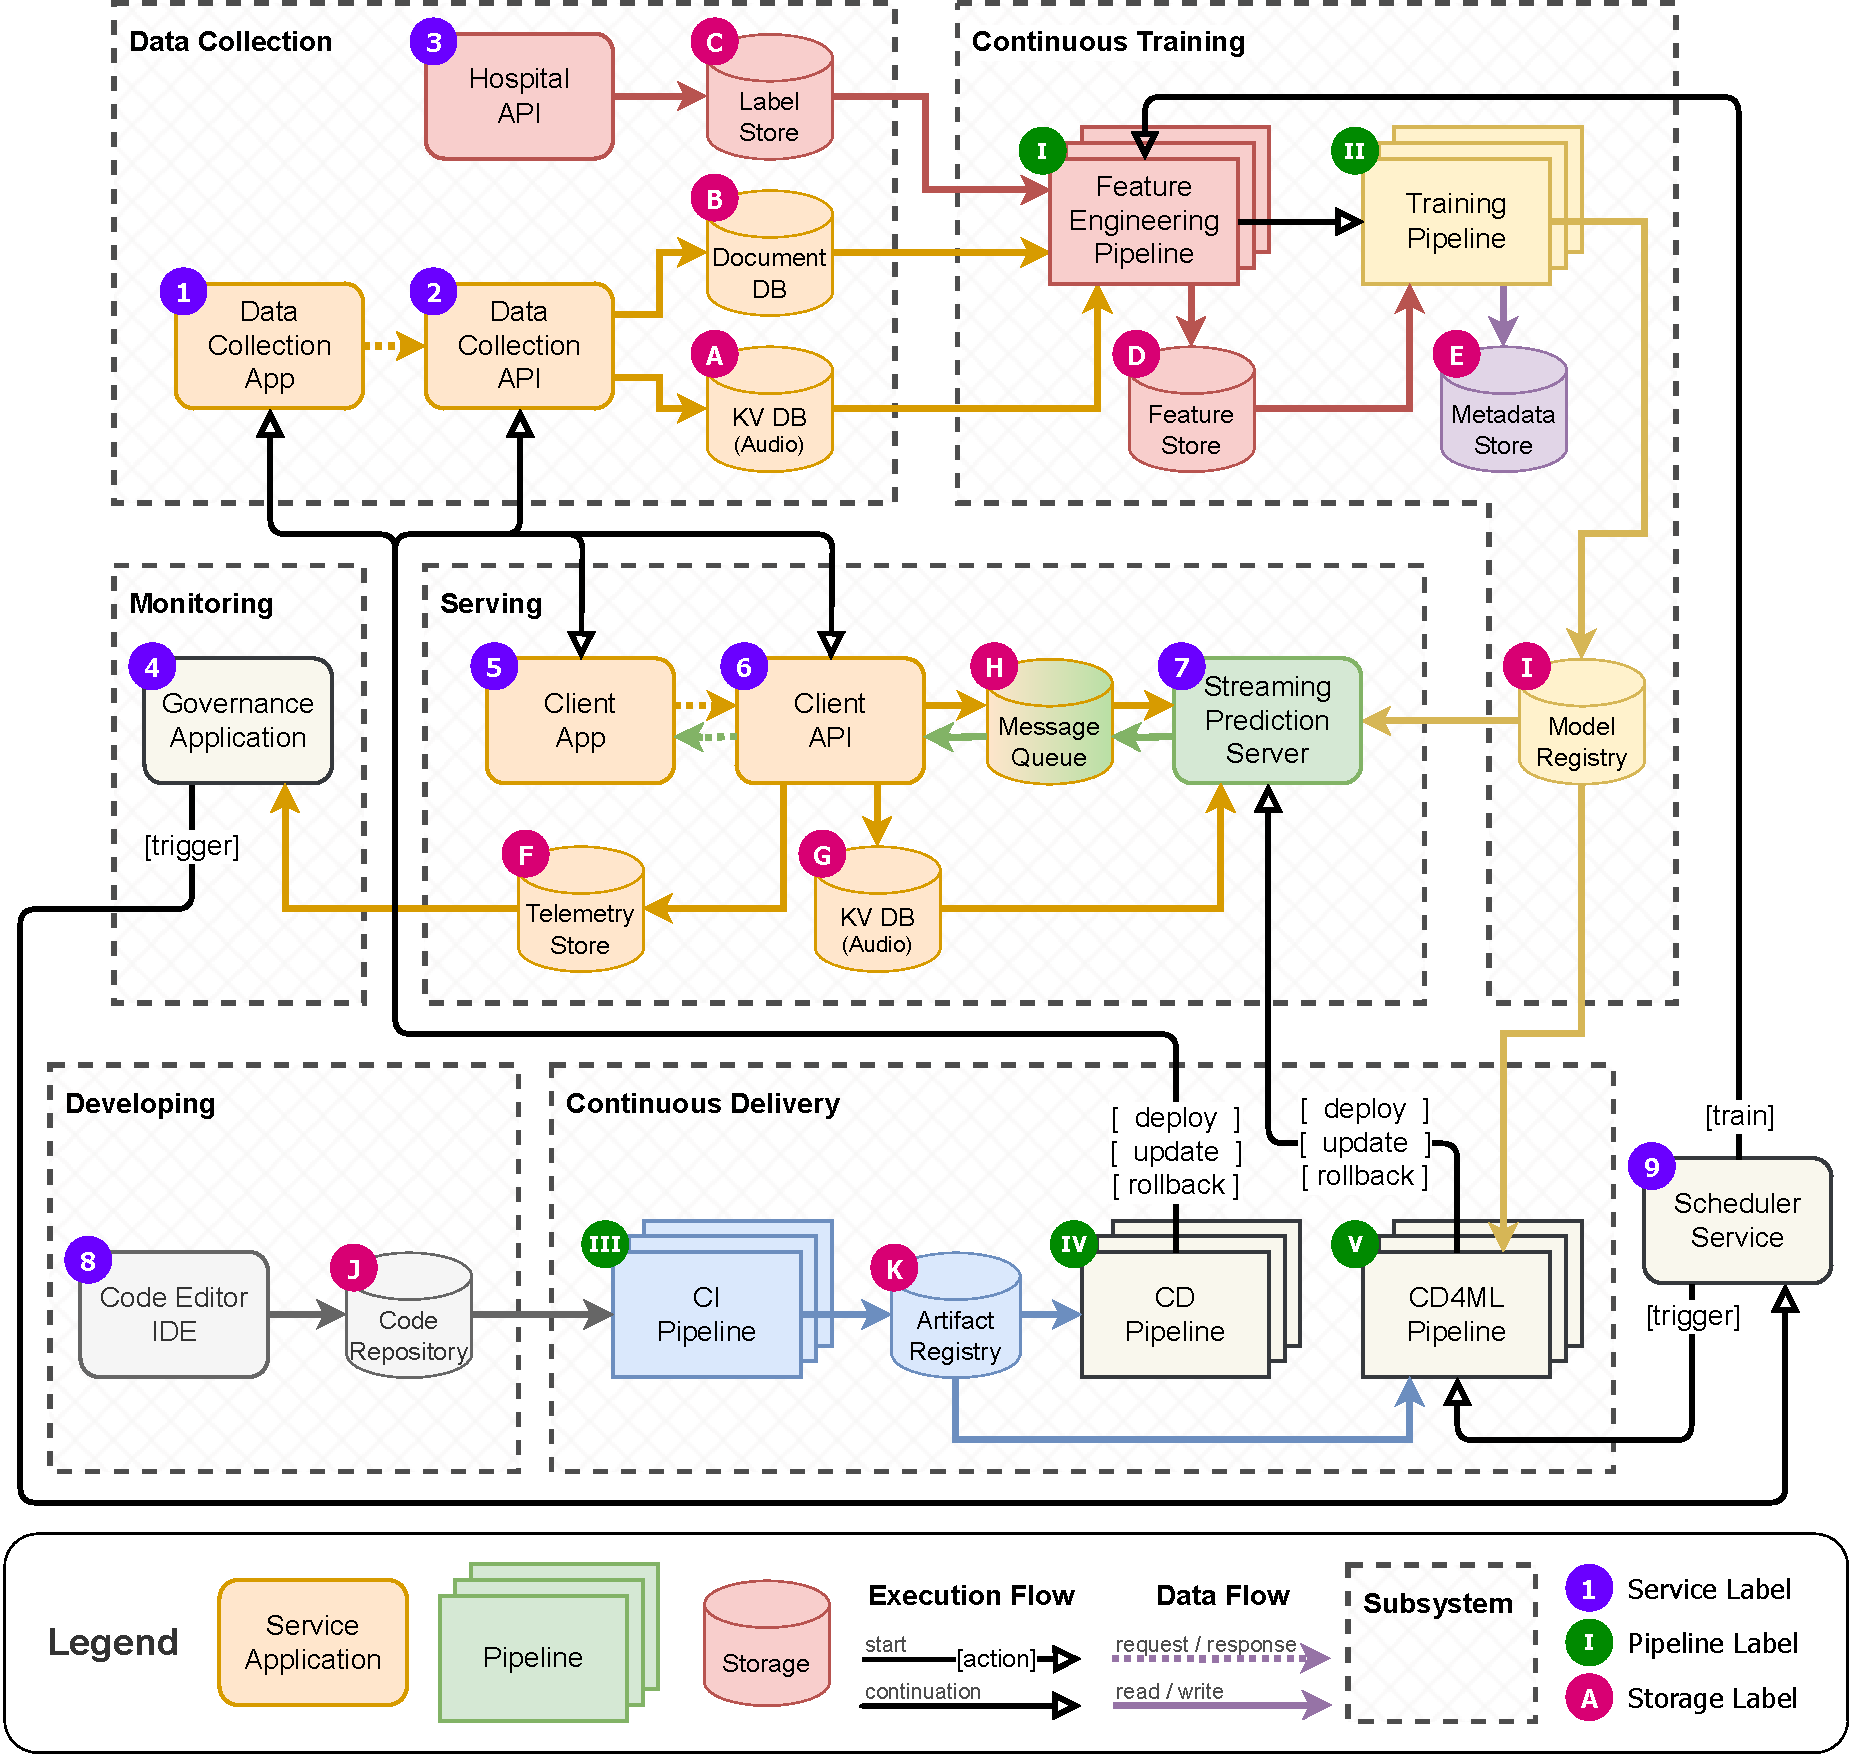
\includegraphics[width=\linewidth]{figures/SPIRA.pdf}
  \caption[%
    Architecture of the SPIRA ML-enabled system%
  ]{%
    \emph{Architecture of the SPIRA ML-enabled system.}
    This architecture follows the same notation presented in
    \cref{fig:reference_architecture}.
    Rectangles represent \textbf{applications} or \textbf{services},
      which execute continuously.
    Stacked rectangles represent \textbf{pipelines},
      which execute a task on demand.
    Lastly, cylinders represent \textbf{data storage},
      which may be databases of any type.
    Components are connected by arrows.
    Black arrows with a hollow tip illustrate the \textbf{execution flow}.
      They start and end in a component.
      Labeled arrows represent the trigger that starts a workflow,
      whereas unlabeled arrows represent the continuation of an
      existing workflow.
    Colored arrows with a filled tip illustrate the \textbf{data flow}.
    They appear in two types:
      solid arrows going to and from a data storage represent
      write and read operations, respectively;
      dotted arrows represent a sync or async request-response
      communication between components.
    Components are colored according to the data they produce:
      \mbox{\LegendColoredComponent{orange}{raw data}},
      \mbox{\LegendColoredComponent{red}{ML-specific data}},
      \mbox{\LegendColoredComponent{gray}{source code}},
      \mbox{\LegendColoredComponent{blue}{executable artifacts}},
      \mbox{\LegendColoredComponent{yellow}{ML models}},
      \mbox{\LegendColoredComponent{purple}{ML training metadata}},
      \mbox{\LegendColoredComponent{green}{ML model predictions}}, and
      \mbox{\LegendColoredComponent{pink}{ML model metrics}}.
      Remaining \LegendBWComponent{standalone components} orchestrate
      the execution of others.
    Components are also grouped into \textbf{subsystems}.
    \LegendColoredLabel{violet}{Numbers},
    \LegendColoredLabel{moss}{roman numerals} and
    \LegendColoredLabel{magenta}{letters}
    are used as labels throughout \cref{chap:the_spira_system}.
  }
  \label{fig:spira_architecture}
\end{figure}
%----------------------------------------------------------------------------%

To create a tool that could assist physicians, the SPIRA team proposed
to develop an ML-enabled system. \Cref{fig:spira_architecture}
presents its system architecture, designed in the early days of this PhD
research~\parencite{Ferreira2022SPIRA:Detection}.
This section discusses how this architecture matches the reference
architecture in \cref{chap:ml_enabled_systems}.
Moreover, it explains how its components have been developed since 2021
through different projects supervised in the context of this research.
In 2022, the experience report \emph{\citetitle{Ferreira2022SPIRA:Detection}}%
~\parencite{Ferreira2022SPIRA:Detection}, was published in the 2nd Workshop
of Intelligent Software Engineering (ISE) at the Brazilian Conference on
Software: Practice and Theory (CBSoft).

A proof of concept of the SPIRA Machine Learning (ML) model was
published in the journal paper \emph{\citetitle{Casanova2021DeepSpeech}}%
~\parencite{Casanova2021DeepSpeech}. To detect respiratory insufficiency
via voice, \citeauthor{Casanova2021DeepSpeech} proposed using
a Convolutional Neural Network (CNN) with multiple hidden layers%
~\parencite{IanGoodfellow2016DeepLearning,RussellS2021Artificial4th},
which could process audio signals recorded in a protocol.
Once they showed the problem could be solved, the next step
was to design an ML-enabled system that could support the proposed
model lifecycle. This way, the SPIRA team would have the means to
incrementally develop and test improvements to their solution.

% The next sections describe the components of the SPIRA system,
% as illustrated by \cref{fig:spira_architecture}. They are grouped
% according to the subsystems presented at \cref{sec:reference_architecture}. 
% On a note, the \cref{sec:spira_serving} subsystem also includes components
% of the client application, since the client was also developed in the
% context of the project.

  \section{Data Collection.}\label{sec:spira_data_collection}
  %%%%%%%%%%%%%%%%%%%%%%%%%%%%%%%%%%%%%%%%%%%%%%%%%%%%%%%%%%%%%%%%%%%%%%%%%%%%
  Creating an ML model that can detect respiratory insufficiency
  via voice is a supervised machine learning classification problem%
  ~\parencite{Casanova2021DeepSpeech}. As such, as explained in
  \cref{sec:ref_data_acquisition}, it requires \emph{labeled data}.
  For the proof of concept, \citeauthor{Casanova2021DeepSpeech}
  used samples obtained in an open survey form shared on the web.
  In the early days of the pandemic, this idea worked well,
  since many people were getting infected (unbeknownst to them).
  Therefore, the odds of finding positive and negative examples
  in the population were high.
  
  When the COVID-19 pandemic started becoming under control, the only
  way to reliably find people with respiratory insufficiency were in the
  hospitals. For that reason, in 2022, the SPIRA team started the development
  of a \LegendService{1}{data collection app}, which could be used by volunteer
  data collectors (working in hospitals) to gather voices.
  This Progressive Web App (PWA) would send the data to a
  \LegendPipeline{2}{data collection API}, which in turn would
  store audio in an \LegendDataStore{A}{audio key-value database}, and
  save patients' demographic data in a \LegendDataStore{B}{document database}.
  These components were developed in the supervision of a scientific
  initiation by the bachelor student Francisco Eugenio Wernke, who developed
  them as part of the course MAC0215 -- ``Undergraduate Research'' at IME-USP.
  %--------------------------------------------------------------------------%
  \begin{supervision}
    \label{sup:ic_francisco}
    \noindent\textbf{%
      Developing a PWA for Collecting Voice for the SPIRA Project.
    }
  
    \noindent%
    \emph{%
      Francisco Eugenio Wernke,
      Renato Cordeiro Ferreira,
      Alfredo Goldman.
    }
  \noindent%
    Scientific Initiation (Bachelor of Computer Science).
  
    \noindent%
    Institute of Mathematics and Statistics, University of São Paulo, 2021.
  \end{supervision}
  %--------------------------------------------------------------------------%
  
  After each collect, data collectors registered an identifier
  (RGH, \EnToBr{Registro Geral Hospitalar}) for each participant.
  This identifier could later be cross-referenced with data shared by each
  partner hospitals via \LegendService{3}{Hospital APIs}. This way, the
  researchers could create a \LegendDataStore{C}{label store} that
  would provide a \emph{ground truth} for the system.
  
  \section{Continuous Training.}\label{sec:spira_continuous_training}
  %%%%%%%%%%%%%%%%%%%%%%%%%%%%%%%%%%%%%%%%%%%%%%%%%%%%%%%%%%%%%%%%%%%%%%%%%%%%
  The next step to productionize SPIRA was to enable continuous training.
  The proof-of-concept code shared by \citeauthor{Casanova2021DeepSpeech}
  could be transformed into two new components:
    a \LegendPipeline{I}{feature engineering pipeline},
    to handle all data processing steps to make audio signals consumable
    by the training algorithm; and
    a \LegendPipeline{II}{training pipeline}, to train and validate the CNN
    proposed in the proof of concept~\parencite{Casanova2021DeepSpeech}.
  
  As explained in \cref{sec:ref_continuous_training}, the creation of these
  two pipelines is an opportunity to introduce standard machine learning
  design patterns~\parencite{Lakshmanan2020MachineMLOps}, such as
    a \LegendDataStore{D}{feature store},
    a \LegendDataStore{E}{metadata store}, and
    a \LegendDataStore{I}{model registry}.
  For the purposes of the project, the suggestion was to use
  \href{https://mlflow.org}{MLFlow} to make the two latter roles.
  On the other hand, for the features, the proposal was to use a
  simple key-value database like \href{https://min.io}{MinIO},
  since a full-featured tool like \href{https://feast.dev}{Feast}
  would be overkill for managing features for a single ML-enabled system.
  
  The implementation of the \nameref{sec:spira_continuous_training}
  subsystem was split into two parts. In 2023, the bachelor student
  Daniel Lawand studied the codebase published by
  \citeauthor{Casanova2021DeepSpeech}~\parencite{Casanova2021DeepSpeech},
  to propose a redesign to its structure. The goal was to evaluate how
  to clean the experimental code, focusing on maintainability.
  This project was supervised as part of Daniel's capstone project.
  In late 2023, it was partially developed in an exchange
  to the Jheronimus Academy of Data Science (JADS) in the Netherlands.
  %--------------------------------------------------------------------------%
  \begin{supervision}
    \label{sup:tcc_daniel}
    \noindent\textbf{%
      Enabling MLOps in the SPIRA training pipeline.
    }
  
    \noindent%
    \emph{%
      Daniel Lawand,
      Renato Cordeiro Ferreira,
      Alfredo Goldman.
    }
  
    \noindent%
    Capstone Project (Bachelor of Computer Science).
  
    \noindent%
    Institute of Mathematics and Statistics, University of São Paulo, 2023.
  \end{supervision}
  %--------------------------------------------------------------------------%
  
  In 2024, the bachelor students Lucas Quaresma and Roberto Bolgheroni
  are continuing this task. Their goal is to implement the design proposal
  made by Daniel Lawand. This project was supervised as part of Lucas's
  and Roberto's group capstone projects. In late 2024, it will be concluded
  in an upcoming exchange of the students to the Jheronimus Academy of
  Data Science (JADS) in the Netherlands.
  %--------------------------------------------------------------------------%
  \begin{supervision}
    \label{sup:tcc_lucas_roberto}
    \noindent\textbf{%
      Productionizing the SPIRA Continuous Training Pipeline.
    }
  
    \noindent%
    \emph{%
      Lucas Quaresma,
      Roberto Bolgheroni,
      Renato Cordeiro Ferreira,
      Alfredo Goldman.
    }
  
    \noindent%
    Capstone Project (Bachelor of Computer Science).
  
    \noindent%
    Institute of Mathematics and Statistics, University of São Paulo, 2024.
  \end{supervision}
  %--------------------------------------------------------------------------%
  
  \section{Serving}\label{sec:spira_serving}
  %%%%%%%%%%%%%%%%%%%%%%%%%%%%%%%%%%%%%%%%%%%%%%%%%%%%%%%%%%%%%%%%%%%%%%%%%%%%
  
  Given SPIRA was meant to be used in hospitals, the client application
  needs to be prepared for this environment. Among the challenges,
  hospitals can have poor internet reception, considering the way
  their building are built (with many corridors and walls).
  As a consequence, the \LegendService{5}{client app} needs to store
  all data collected locally \emph{before} sending them to the cloud,
  thus preventing problems with an unreliable network. This implies
  the \LegendService{6}{client API} should also make a checksum of
  any data received to ensure everything no data was corrupted before
  storing it in its \LegendDataStore{G}{audio key-value database}.
  Moreover, data will likely arrive in \emph{bursts}, i.e., multiple
  audios will be sent together by the \LegendService{5}{client app}
  when the data collector gets internet access.
  
  To handle an arbitrarily large, unforeseeable, on-demand number
  of predictions, SPIRA should rely on a \LegendService{7}{streaming
  prediction service}. It will queue all prediction requests in a
  \LegendDataStore{H}{message queue}, then return the predictions
  results through it. This solution also makes it easier to manage
  the execution of the server.
  The model proposed by \citeauthor{Casanova2021DeepSpeech} -- a CNN with
  multiple layers -- is a model that requires accelerator hardware (GPUs)
  to run efficiently~\parencite{IanGoodfellow2016DeepLearning}.
  The \LegendService{7}{streaming prediction service} can be run
  in a specialized machine, whereas other components may be
  deployed in cheaper hardware.
  
  The implementation of the \nameref{sec:spira_serving} subsystem was also
  split in two parts. In 2022, the bachelor student Vitor Tamae developed
  all the components in the subsystem.
  %--------------------------------------------------------------------------%
  \begin{supervision}
    \label{sup:tcc_tamae}
    \noindent\textbf{%
      Building an Intelligent System to Detect Respiratory Insufficiency.
    }
  
    \noindent%
    \emph{%
      Vitor Daisuke Tamae,
      Renato Cordeiro Ferreira,
      Marcelo Finger,
      Alfredo Goldman.
    }
  
    \noindent%
    Capstone Project (Bachelor of Computer Science).
  
    \noindent%
    Institute of Mathematics and Statistics, University of São Paulo, 2022.
  \end{supervision}
  %--------------------------------------------------------------------------%
  
  In 2023, the bachelor student Vitor
  Guidi continued this effort by investigating how to deploy all this
  infrastructure in a \href{https://kubernetes.io/}{Kubernetes}-managed
  cluster of machines. Both projects were supervised as part of the
  students' capstone projects.
  %--------------------------------------------------------------------------%
  \begin{supervision}
    \label{sup:tcc_guidi}
    \noindent\textbf{%
      Cloud-Native Machine Learning: \\
      Enabling High Availability to the SPIRA System with Kubernetes.
    }
  
    \noindent%
    \emph{%
      Vitor Guidi,
      Renato Cordeiro Ferreira,
      Alfredo Goldman.
    }
  
    \noindent%
    Capstone Project (Bachelor of Computer Science).
  
    \noindent%
    Institute of Mathematics and Statistics, University of São Paulo, 2023.
  \end{supervision}
  %--------------------------------------------------------------------------%
  
  \section{Monitoring.}\label{sec:spira_monitoring}
  %%%%%%%%%%%%%%%%%%%%%%%%%%%%%%%%%%%%%%%%%%%%%%%%%%%%%%%%%%%%%%%%%%%%%%%%%%%%
  Another desirable capability for the SPIRA system is AB-testing,
  so it may be possible to train and test multiple variants of the SPIRA
  CNN to improve its modelling. As part of his capstone project,
  while implementing the \nameref{sec:spira_serving} subsystem,
  the bachelor student Vitor Tamae made the \LegendService{6}{client API}
  to support calling multiple models at the same time. This capability is
  the inception of a \LegendService{4}{governance application}, which will
  allow the researchers to track the system usage stored in a
  \LegendDataStore{F}{telemetry store}.
  
  \section{Development.}
  \label{sec:spira_development_ci}
  %%%%%%%%%%%%%%%%%%%%%%%%%%%%%%%%%%%%%%%%%%%%%%%%%%%%%%%%%%%%%%%%%%%%%%%%%%%%
  The last step to support further experimentation with the SPIRA model
  is to provide the capability to quickly experiment with multiple systems.
  Currently, data scientists can access SPIRA source code in an open
  \LegendDataStore{J}{code repository} at GitHub%
  \footnote{https://github.com/spirabr}.
  Any changes may be made using standard development tools:
  \LegendService{8}{code editors} or \LegendService{8}{IDEs},
  according to the preference of the SPIRA team.
  
  \section{Continuous Delivery.}
  \label{sec:spira_continuous_delivery}
  %%%%%%%%%%%%%%%%%%%%%%%%%%%%%%%%%%%%%%%%%%%%%%%%%%%%%%%%%%%%%%%%%%%%%%%%%%%%
  Taking advantage of the use of \href{https://github.com}{GitHub},
  the bachelor students Lucas Quaresma and Roberto Bolgheroni are currently
  building the \nameref{sec:spira_continuous_delivery} components to make
  it easy to build, test, and deploy new versions of SPIRA.
  The \LegendService{III}{CI pipeline} is being built using GitHub actions,
  to generate \href{https://www.docker.com/}{Docker} containers of the
  various components that are part of SPIRA. These containers will be
  deployed in the GitHub Container Registry%
  \footnote{https://github.blog/2020-09-01-introducing-github-container-registry/},
  which will be the \LegendDataStore{K}{artifact store} for SPIRA.
  
  During 2024, as part of their capstone project, the students
  Lucas Quaresma and Roberto Bolgheroni will also develop the
  \LegendPipeline{IV}{CD} and \LegendPipeline{V}{CD4ML} pipelines.
  They will use the infrastructure configuration developed by Vitor Guidi
  in 2023 to create a process to deploy, update, and rollback all components
  in a \href{https://kubernetes.io/}{Kubernetes}-managed cluster.

%!tex root=../thesis.tex
%("dica" para o editor de texto: este arquivo é parte de um documento maior)
% para saber mais: https://tex.stackexchange.com/q/78101/183146

\chapter{Research Methodology}
\label{chap:research_methodology}
%%%%%%%%%%%%%%%%%%%%%%%%%%%%%%%%%%%%%%%%%%%%%%%%%%%%%%%%%%%%%%%%%%%%%%%%%%%%%%%%

%!TeX root=../thesis.tex
%("dica" para o editor de texto: este arquivo é parte de um documento maior)
% para saber mais: https://tex.stackexchange.com/q/78101/183146

\chapter{Work Plan}
\label{chap:work_plan}
%%%%%%%%%%%%%%%%%%%%%%%%%%%%%%%%%%%%%%%%%%%%%%%%%%%%%%%%%%%%%%%%%%%%%%%%%%%%%%%%

This PhD research started at University of São Paulo (USP) in late 2020.
Besides the challenges of the COVID-19 pandemic, the author was working in
a full-time job as \emph{principal machine learning engineer} at
\href{https://www.elo7.com.br}{Elo7} -- an experience that inspired
this research. In 2023, this PhD started being developed in a sandwich
doctorate in the Jheronimus Academy of Data Science (JADS) in the Netherlands.
Since 2024, the author has been employed as a \emph{scientific programmer}
in the \href{https://marit-d.eu/}{MARIT-D European project}.

This chapter presents a work plan to execute the research methodology
from \cref{chap:research_methodology}. The timeline considers this PhD
is not a full-time activity. \Cref{tab:work_plan} accounts time to:
%------------------------------------------------------------------------------%
\begin{itemize}
  \item execute each step of the methodology,
  \item submit publications about the results of each phase of the methodology, and
  \item write the thesis for final submission.
\end{itemize}
%------------------------------------------------------------------------------%

%------------------------------------------------------------------------------%
\begin{table}[b!]
  \centering
  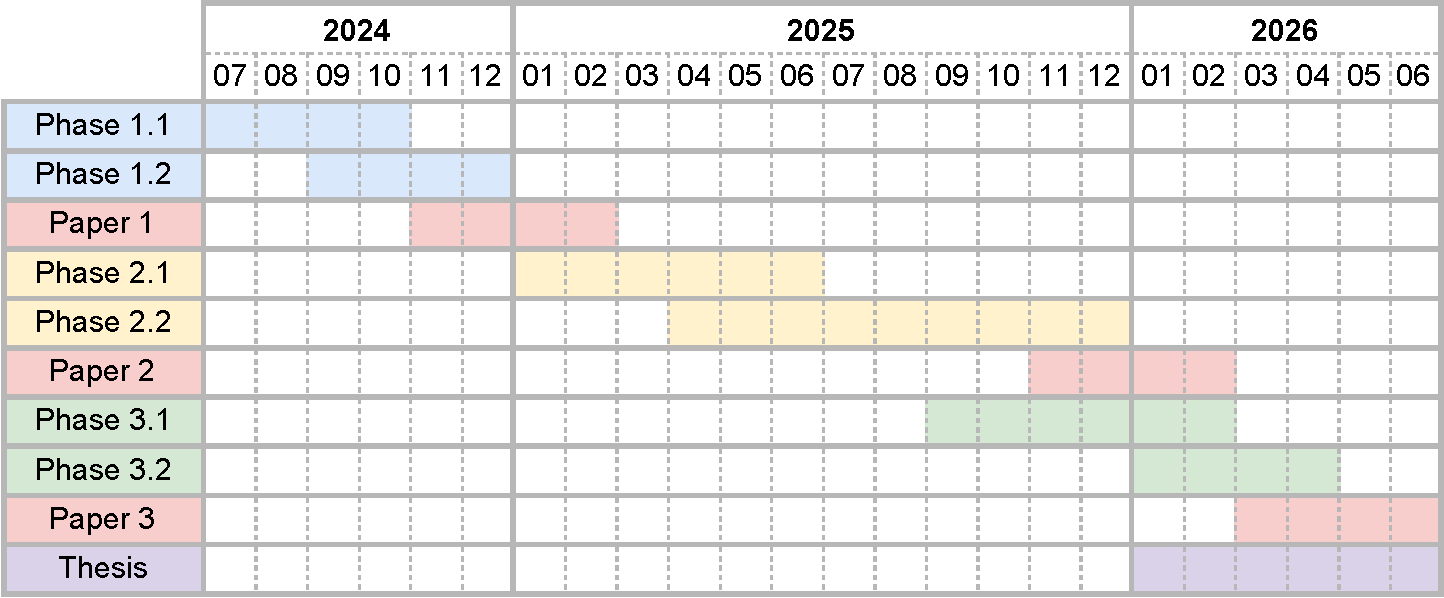
\includegraphics[width=0.85\linewidth]{tables/Timetable.pdf}
  \caption[%
    Work plan%
  ]{%
    \emph{Work Plan}. The timetable summarizes the expected number
    of months to complete the research methodology introduced in
    \cref{chap:research_methodology}. Each line represents a task,
    each column represents a month. Lines and cells are color-coded
    according to \cref{fig:research_methodology}.
  }
  \label{tab:work_plan}
\end{table}
%------------------------------------------------------------------------------%
% %!TeX root=../thesis.tex
%("dica" para o editor de texto: este arquivo é parte de um documento maior)
% para saber mais: https://tex.stackexchange.com/q/78101/183146

\chapter{Measuring Complexity}
\label{chap:measuring_complexity}
%%%%%%%%%%%%%%%%%%%%%%%%%%%%%%%%%%%%%%%%%%%%%%%%%%%%%%%%%%%%%%%%%%%%%%%%%%%%%%%%

%%%%%%%%%%%%%%%%%%%%%%%%%%%% APÊNDICES E ANEXOS %%%%%%%%%%%%%%%%%%%%%%%%%%%%%%%%

% Um apêndice é algum conteúdo adicional de sua autoria que faz parte e
% colabora com a ideia geral do texto mas que, por alguma razão, não precisa
% fazer parte da sequência do discurso; por exemplo, a demonstração de um
% teorema intermediário, as perguntas usadas em uma pesquisa qualitativa etc.
%
% Um anexo é um documento que não faz parte da tese (em geral, nem é de sua
% autoria) mas é relevante para o conteúdo; por exemplo, a especificação do
% padrão técnico ou a legislação que o trabalho discute, um artigo de jornal
% apresentando a percepção do público sobre o tema da tese etc.
%
% Os comandos appendix e annex reiniciam a numeração de capítulos e passam
% a numerá-los com letras. "annex" não faz parte de nenhuma classe padrão,
% foi criado para este modelo. Se o trabalho não tiver apêndices ou anexos,
% remova estas linhas.
%
% Diferentemente de \mainmatter, \backmatter etc., \appendix e \annex não
% forçam o início de uma nova página. Em geral isso não é importante, pois
% o comando seguinte costuma ser "\chapter", mas pode causar problemas com
% a formatação dos cabeçalhos. Assim, vamos forçar uma nova página antes
% de cada um deles.

%%%% Apêndices %%%%

\makeatletter
\if@openright\cleardoublepage\else\clearpage\fi
\makeatother

\pagestyle{appendix}

\appendix

% \addappheadtotoc acrescenta a palavra "Apêndice" ao sumário; se
% só há apêndices, sem anexos, provavelmente não é necessário.
\addappheadtotoc

%!TeX root=../thesis.tex
%("dica" para o editor de texto: este arquivo é parte de um documento maior)
% para saber mais: https://tex.stackexchange.com/q/78101/183146

\chapter{Related Activities}
\label{app:related_activities}
%%%%%%%%%%%%%%%%%%%%%%%%%%%%%%%%%%%%%%%%%%%%%%%%%%%%%%%%%%%%%%%%%%%%%%%%%%%%%%%%
  
Since the beginning of this PhD, the candidate has been involved in many
academic activities related to his research topic. This appendix summarizes them.

\paragraph{Publications.}
Since 2020, the following papers were co-authored as part of this research:
%----------------------------------------------------------------------------%
\begin{enumerate}
  \item \fullcite{Ferreira2024BeingProject}
  \item \fullcite{Durelli2022UsingPractices}
  \item \fullcite{Ferreira2022SPIRA:Detection}
  \item \fullcite{Finger2021DetectingProject}
  \item \fullcite{Ferreira2020H.I.D.R.A.:Categorization}
  \item \fullcite{Ferreira2020TeachingMicroservices}
\end{enumerate}
%------------------------------------------------------------------------------%

\paragraph{Supervisions.}
Since 2020, the authors have supervised many projects related to
\emph{Software Engineering for Artificial Intelligence} (SE4AI), including:
%----------------------------------------------------------------------------%
\begin{itemize}
  \item \emph{13 capstone projects}
        in Computer Science at IME-USP (Brazil);
  \item \emph{6 undergraduate research projects}
        in Computer Science at IME-USP (Brazil);
  \item \emph{2 professional masters}
        in Applied Computer Science at IPT (Brazil); and
  \item \emph{3 masters of science}
        in Data Science and Entrepreneurship at JADS (Netherlands).
\end{itemize}
%------------------------------------------------------------------------------%

\paragraph{Teaching.}
Since 2020, the authors have been involved in many teaching activities,
which contributed to publications and inspired ideas for this PhD:
%------------------------------------------------------------------------------%
\begin{itemize}
  \item \href{https://uspdigital.usp.br/jupiterweb/obterDisciplina?sgldis=MAC0475}%
        {MAC0415 -- Laboratory of Complex Computational Systems}, \\
        offered to the Bachelor of Computer Science at IME-USP (2020.1 / 2021.1);
  \item \href{https://uspdigital.usp.br/jupiterweb/obterDisciplina?sgldis=MAC0472}%
        {MAC0472 -- Laboratory of Agile Methods}, \\
        offered to the Bachelor of Computer Science at IME-USP (2020.2 / 2021.2);
  \item \href{https://uspdigital.usp.br/jupiterweb/obterDisciplina?sgldis=MAC0218}%
        {MAC0218 -- Programming Techniques II}, \\
        offered to the Bachelor of Computer Science at IME-USP (2022.1);
  \item \href{https://uspdigital.usp.br/apolo/apoObterAtividade?cod_oferecimentoatv=99168}%
        {Development of Intelligent Systems}, \\
        offered as a summer course at IME-USP (2021 / 2022); and
\end{itemize}
%----------------------------------------------------------------------------%

\par

% %%%% Anexos %%%%

% \makeatletter
% \if@openright\cleardoublepage\else\clearpage\fi
% \makeatother

% \pagestyle{appendix} % repete o anterior, caso você não use apêndices

% \annex

% % \addappheadtotoc acrescenta a palavra "Anexo" ao sumário; se
% % só há anexos, sem apêndices, provavelmente não é necessário.
% \addappheadtotoc

% %\input{conteudo/anexo-exemplo-faq}
% \par


%%%%%%%%%%%%%%% SEÇÕES FINAIS (BIBLIOGRAFIA E ÍNDICE REMISSIVO) %%%%%%%%%%%%%%%%

% O comando backmatter desabilita a numeração de capítulos.
\backmatter

\pagestyle{backmatter}

% Espaço adicional no sumário antes das referências / índice remissivo
\addtocontents{toc}{\vspace{2\baselineskip plus .5\baselineskip minus .5\baselineskip}}

% A bibliografia é obrigatória
\printbibliography[
  title=\refname\label{bibliografia}, % "Referências", recomendado pela ABNT
  %title=\bibname\label{bibliografia}, % "Bibliografia"
  heading=bibintoc, % Inclui a bibliografia no sumário
]

% \printindex % imprime o índice remissivo no documento (opcional)

\end{document}
